\chapter{Neutron Transport \& Diffusion}

The behavior of a nuclear fission reactor is primarily governed by the distribution of nuclear fission events throughout the system. To model this, we need to be able to predict the behavior of the neutrons causing those fissions. Our task therefore is to develop a mathematical description for predicting how the distribution of neutrons within the reactor evolves with time. The field of study associated with this is referred to as \emph{neutronics}. 

There are two models that are used. The first is called \emph{neutron transport}, which models the positions and velocities of neutrons throughout the reactor. In classical physics, if we know the position and velocity of a bunch of objects, we can predict the future of those objects. There are three components of position and three components of velocity. And this implies that we have six dimensions that need to be considered in addition to time. As such, the equations of neutron transport are very difficult to solve, only having few analytical solutions in exceptionally simplistic cases, and the numerical schemes for obtaining approximate solutions form a discipline unto itself. 

Fortunately, neutron transport is not needed for a large class of problems encountered in reactor physics, particularly ones involving finding the distribution over a large geometrical region of the reactor. There is a much simpler model called \emph{neutron diffusion} that is valid in the limit that neutron scattering dominates the effects of neutron streaming and absorption. The neutron diffusion model does not explicitly account for the directionality of the neutrons, effectively reducing the dimensionality of the problem to four plus another for time. Three of these are for spatial position and another for the distribution of kinetic energies of neutrons. Another important feature of neutron diffusion is that it is mathematically similar in structure to the equations encountered in fluid and heat transport, and are therefore far better understood and significantly easier to solve.

One might be wondering about the role of quantum mechanics. Because the nuclear interactions occur at very localized positions over a rapid time interval, we can decouple the random quantum behavior from the equations of motion for the neutrons. All of the quantum physics gets lumped into parameters within these equations, which are our cross sections from the nuclear data.

%%%%%%%%%%%%%%%%%%%%%%%%%%%%%%%%%%%%%%%%%%%%%%%%%%%%%%%%%%%%%%%%%%%%%%%%%%%%%%%%
\section{Neutron Transport}

Our goal is to develop a semiclassical theory where the transport of neutrons is governed by the standard equations of motion where the quantum mechanical details are handled on average through cross section coefficients. To help with this, we make the following assumptions:
\begin{enumerate}
  \item The neutrons are point-like objects having no internal structure that can be characterized by a well-defined position $(x,y,z)$ and velocity vector $\mathbf{v} = ( v_x, v_y, v_z )$ or energy $E$ and unit vector $\dir$.
  \item Neutrons travel in straight-line trajectories. In this, we neglect the effect of gravity on neutrons and this leads to there being no preferred direction in the reactor. (This assumption turns out to be valid because the time of neutron trajectories between collisions are too short for gravity to have much influence.)
  \item Neutron interactions with nuclei occur at well-defined, random (exponentially distributed) locations in space with coefficients that probabilistically describe the physics of those interactions. These coefficients are obtained from the nuclear data.
  \item The density of neutrons is low enough that the rate that neutrons collide with other neutrons is low enough to be ignored.
\end{enumerate}
From these assumptions, we could, in principle, write down an equation for each neutron in the reactor. Given the sheer number of neutrons in an operating reactor at any given time, which could be upwards of $10^{10}$ neutrons every cubic centimeter, this problem would obviously be infeasible to solve directly. That said, we can and do formulate these equations and simulate them for numerous random neutron interactions. If we do a large number of them, we can make inferences about the neutron field and fission distribution. This is called the Monte Carlo method and is one of the techniques used in neutronics. While very powerful, it is computationally expensive and rarely used for routine analyses.

\subsection{Neutron Density \& Angular Flux}

The alternative to modeling every individual neutron is to describe the neutrons using a statistical density function. Here we introduce the expected or mean neutron population as a function of position and velocity. This density function can be defined as follows:
\begin{align}
  n(\pos,\dir,E,t) dV d\Omega dE = 
  &\text{ the expected (mean) population of neutrons at some } \nonumber \\*
  &\text{ position $\pos$ centered about differential volume $dV$, } \nonumber \\*
  &\text{ traveling with direction $\dir$ within  some patch of } \nonumber \\*
  &\text{ solid angle $d\Omega$, having kinetic energy between } \nonumber \\*
  &\text{ $E$ and $E + dE$ at time $t$.} \nonumber
\end{align}
The units of this density function $n(\pos,\dir,E,t)$ are neutrons per unit volume, per unit solid angle, per unit energy. 

While the neutron density is a nice fundamental quantity, it is impossible to measure because we can only detect neutrons when they interact with matter. To arrive at such a quantity, we use a thought experiment. To begin, let us consider a beam of neutrons all having equivalent velocity or direction $\dir$ and energy $E$. Next, we will place a small circular surface with an orientation given by a unit normal vector $\nhat$ (different than the direction of the neutrons) with a differential area $dA$. 

\begin{figure}[tb!]
\begin{center}
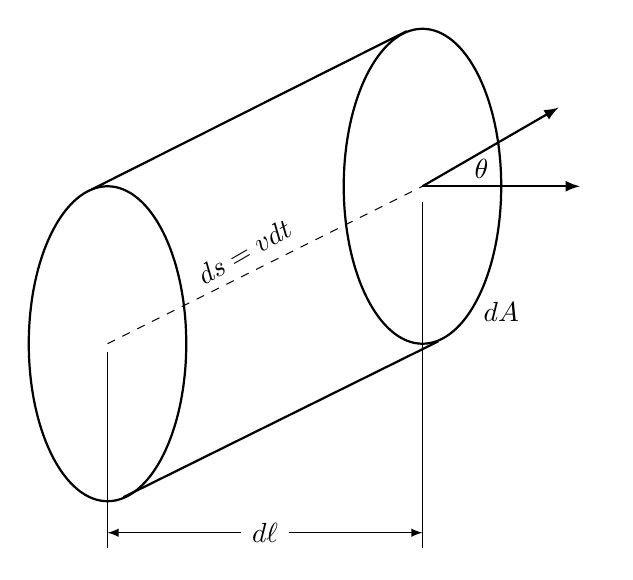
\begin{tikzpicture}
   \draw[thick] (0,0) ellipse (1cm and 2cm);
   \draw[thick] (-4,-2) ellipse (1cm and 2cm);
   \draw[thick] (-4.2,-0.04) -- (-0.2,1.97);
   \draw[thick] (-3.8,-3.95) -- (0.2,-1.97);
   \draw[-latex,thick] (0,0) -- (2,0);
   \draw[-latex,thick] (0,0) -- (1.73,1);
   \node at (2.2,0.2) {$\nhat$};
   \node at (1.6,1.6) {$\dir$};
   \draw[dashed] (-4,-2) -- (0,0);
   \node[rotate around={30:(-1.4,-1.35)}] at (-1.4,-1.35) {$ds = vdt$};
   \draw ( 0,-0.2) -- ( 0,-4.6);
   \draw (-4,-2.1) -- (-4,-4.6);
   \draw[-latex] (-2.3,-4.4) -- (-4,-4.4);
   \draw[-latex] (-1.7,-4.4) -- ( 0,-4.4);
   \node at (-2,-4.4) {$d\ell$};
   \node at (1.0,-1.6) {$dA$};
   \node at (0.75,0.225) {$\theta$};
\end{tikzpicture}
\caption{Differential volume containing all neutrons crossing the surface $dA$ in time interval $dt$.}
\label{Fig:neutronics_dV_neutronsCrossing}
\end{center}
\end{figure}

Now we want to count the number of neutrons that cross this surface in some time interval from $t$ to $t + dt$. We can reason that any neutron within some cylindrical volume with sheered edges depicted in Fig.~\ref{Fig:neutronics_dV_neutronsCrossing}. (Imagine a pipe oriented at an angle with respect to the ground where we slice the pipe vertically.) The distance $ds$ along the axis of the cylinder oriented with $\dir$ can be related to the the time interval by $ds = vdt$. The volume of the region $dV$ is the product of the the area $dA$ and the length $d\ell$, which is oriented along the surface $dA$ with unit normal $\nhat$. The length $d\ell$ is related to $ds$ by the cosine of the angle $\theta$ between $\nhat$ and $\dir$, which is given by the dot product between them.

The number of neutrons crossing the surface within time interval $dt$ is equal to the number of the neutrons within volume $dV$, we can write this relationship in terms of the neutron density
\begin{align}
  n(\pos,\dir,E,t) dV d\Omega dE = 
  	&\text{ number of neutrons in the volume} \nonumber \\*
  = &\text{ number of neutrons crossing the surface in the time interval} \nonumber \\*
  =	&\ n(\pos,\dir,E,t) d\ell dA d\Omega dE \nonumber \\
  =	&\ n(\pos,\dir,E,t) ds (\nhat \cdot \dir) dA d\Omega dE \nonumber \\
  = &\ n(\pos,\dir,E,t) (v dt) (\nhat \cdot \dir) dA d\Omega dE \nonumber \\
  = &\ (\nhat \cdot \dir)  [ v n(\pos,\dir,E,t) ] dA d\Omega dE dt. \nonumber 
\end{align}

Inspecting this we notice the term in brackets $vn$, we define the \emph{angular flux} as
\begin{align}
  \psi(\pos,\dir,E,t) = v n(\pos,\dir,E,t) .
\end{align}
This has units of length per volume or per area, per solid angle, per energy, per time. We can give this angular flux one of two interpretations based on our thought experiment. The first is that of a rate crossing a fictitious surface. This formally can be stated as
\begin{align}
  \psi(\pos,\dir,E,t) dA d\Omega dE 
  = &\text{ the rate neutrons traveling with a direction $\dir$ in solid } \nonumber \\*
   	&\text{ angle $d\Omega$ with energy in range $E$ and $E + dE$ cross a} \nonumber \\*
	&\text{ fictitious surface of area $dA$ centered about position $\pos$ } \nonumber \\*
   	&\text{ that is oriented normal to  the direction $\dir$.} \nonumber 
\end{align}

The other interpretation is related to the the reaction rate, which is the one we can measure. The number of reactions that the neutrons undergo between the two edges of this infinitesimal volume is proportional to the distance or path-length $ds$ times the total cross section $\Sigma_t$. This implies the angular flux can be viewed as
\begin{align}
  \psi(\pos,\dir,E,t) dV d\Omega dE 
  = &\text{ the amount of path-length generated by neutrons traveling } \nonumber \\*
   	&\text{ with a direction $\dir$ in solid angle $d\Omega$ with energy in range } \nonumber \\*
   	&\text{ $E$ and $E + dE$ within a convex region having volume $dV$ } \nonumber \\*
   	&\text{centered about position $\pos$.} \nonumber 
\end{align}
Note the units of this expression are length per time. In reality, we will have some finite sized volume with neutrons traveling in a distribution of directions. Suppose our region is convex (any neutron that leaves will not be able to reenter) and we take several paths through it. Because of the results we derived for exponential attenuation, we know that the longer paths will have more interactions compared to the shorter ones. As we shrink the volume of this region down to have infinitesimal size $dV$, the relative ratio of the path lengths will converge to some fixed value. To compute the reaction rate in the differential volume we would ``add up'' the amount of distance for neutrons traveling in each direction and multiply by the cross section.

\begin{figure}[tb!]
\begin{center}
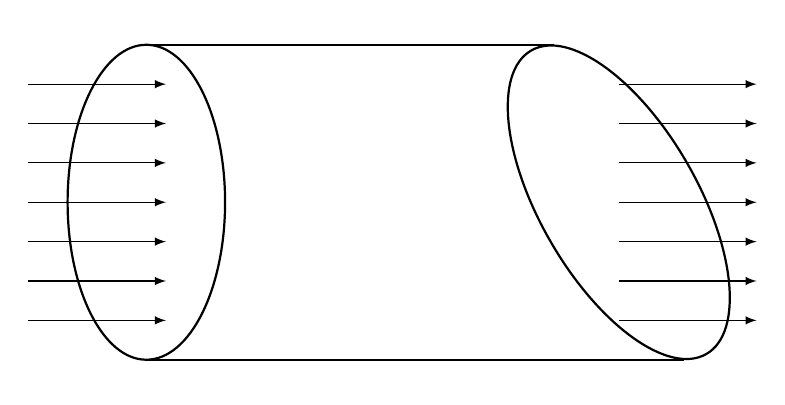
\begin{tikzpicture}
   \draw[thick] (0,0) ellipse (1cm and 2cm);
   \draw[thick, rotate around={30:(6,0)}] (6,0) ellipse (1cm and 2.225cm);
   \draw[thick] (0,2) -- (5.175,2);
   \draw[thick] (0,-2) -- (6.825,-2);

   \foreach \y in {-1.5,-1.0,-0.5,0,0.5,1.0,1.5} {
     \draw[-latex] (-1.5,\y) -- (0.25,\y);
     \draw[-latex] (6.0,\y) -- (7.75,\y);
   }
%   \draw[thick] (-4.2,-0.04) -- (-0.2,1.97);
%   \draw[thick] (-3.8,-3.95) -- (0.2,-1.97);
%   \draw[-latex,thick] (0,0) -- (2,0);
%   \draw[-latex,thick] (0,0) -- (1.73,1);
%   \node at (2.2,0.2) {$\nhat$};
%   \node at (1.6,1.6) {$\dir$};
%   \draw[dashed] (-4,-2) -- (0,0);
%   \node[rotate=30] at (-1.9,-0.6) {$ds = vdt$};
%   \draw ( 0,-0.2) -- ( 0,-4.6);
%   \draw (-4,-2.1) -- (-4,-4.6);
%   \draw[-latex] (-2.3,-4.4) -- (-4,-4.4);
%   \draw[-latex] (-1.7,-4.4) -- ( 0,-4.4);
%   \node at (-2,-4.4) {$d\ell$};
%   \node at (1.0,-1.6) {$dA$};
%   \node at (0.75,0.225) {$\theta$};
\end{tikzpicture}
\caption{Beam of neutrons entering a pipe with edges sheered with different orientations.}
\label{Fig:neutronics_neutronBeamAlongSheeredPipe}
\end{center}
\end{figure}

Before proceeding, note the factor of $\nhat \cdot \dir$, which is the cosine of the angle between the unit normal $\nhat$ of the surface $dA$ and the direction $\dir$ on the number of particles crossing the surface. To conceptualize this, let us consider a beam of neutrons flowing down a pipe, but this time the pipe is sheered along different orientations, as shown in Fig.~\ref{Fig:neutronics_neutronBeamAlongSheeredPipe}. The surfaces at the ends of the pipe have different areas. If we shine a steady beam of neutrons down the pipe, then the rate that neutrons enter must equal the rate they exit. Because the areas are different, we need to multiply by a factor of $\nhat \cdot \dir$ on each end to ensure the amount of neutrons that we calculate with the neutron density is equivalent.

\subsection{Derivation of the Neutron Transport Equation}

Given these quantities, our task is to develop a differential equation that describes how the neutron density function evolves in time. If we can solve this differential equation, we can predict the neutron field and obtain the distribution of fissions throughout the reactor. Fortunately, in the 1800s a physicist named Ludwig Boltzmann (the same one from the Maxwell-Boltzmann distribution) developed the theory of statistical mechanics that be used for this purpose. The eponymously named Boltzmann equation describes the evolution of a distribution function subject to (a) external forces, (b) internal transport, and (c) collisions between themselves and the background materials. In fact, this Boltzmann equation can be used to derive the balance of mass, momentum, and energy that are used to describe the transport of fluids and heat, but that is a topic for a different course.

Back to neutrons, the self-collisions in the Boltzmann equation make the equation nonlinear and difficult to solve. However, since we can neglect neutron-neutron collisions because the neutron density is sufficiently low, we can eliminate this term and reach a form called the linearized Boltzmann equation. To obtain this equation, we once again consider a beam of neutrons traveling the nearly the same direction given by a differential solid angle range $d\Omega$ about some direction $\dir$, and having kinetic energies in some range $E$ and $E + dE$ along with a surface of area $dA$. (The difference from the previous case being now that we choose the orientation of the surface $dA$ such that the unit normal $\nhat$ equals $\dir$.)

Suppose we wish to count the number of neutrons crossing this surface between time interval $t$ and $t + \Delta t$. If all neutrons are traveling with the same speed $v$ and move in the same direction, then we can again draw some cylindrical volume with height $\Delta s = v \Delta t$ and base with area $dA$ such that all neutrons within it at time $t$ are guaranteed to cross the surface. This is called a control volume and will serve the basis for the balance relation. Here we will take the location $\pos$ as the center of the base at the start of the control volume and the position $\pos + \Delta s \dir$ as the location of the top of the control volume. 

The next step is to enumerate the losses and gains within this control volume and equate this with the change in the number of neutrons within the volume between times $t$ and $t + \Delta t$. We are going to reach into our bag of mathematical theorems and pull out the mean-value theorem, which says (assuming the neutron density varies continuously) there is some location between $\pos$ and $\pos + \Delta s \dir$ having the average value of neutrons during that time interval. Let us call this position $\pos + \kappa \Delta s \dir$, where $0 \le \kappa \le 1$. It turns out we will not care what $\kappa$ is, just that it exists. We then can assert that
\begin{align}
  &\left[ n( \pos + \kappa \dir \Delta s , \dir, E, t + \Delta t ) - n( \pos + \kappa \dir  \Delta s , \dir, E, t ) \right] \Delta s dA d\Omega dE \nonumber \\*
  = &\text{ change in the number of neutrons in control volume} \nonumber \\*
  	&\text{ during time interval $t$ and $t + \Delta t$.} 
\end{align} 

Within this time interval, we gain neutrons when they cross the surface at $\pos$ and lose them when they cross the surface at $\pos + \dir \Delta s$. By convention, we will consider the net loss in the number of neutrons, i.e., the number exiting minus entering. Similar to before, we can use the mean-value theorem to take the density function at at a time $t + \epsilon \Delta t$ for $0 \le \epsilon \le 1$ where it has the average value. Again, we will not care what $\epsilon$ is, just that it exists. We have the net loss across the volume as 
\begin{align}
  &\left[ n( \pos + \dir \Delta s , \dir, E, t + \epsilon \Delta t ) - n( \pos , \dir, E, t + \epsilon  \Delta t ) \right] \Delta s dA d\Omega dE \nonumber \\*
  =  &\left[ n( \pos + \dir \Delta s , \dir, E, t + \epsilon  \Delta t ) - n( \pos , \dir, E, t + \epsilon  \Delta t ) \right]  ( v \Delta t ) dA d\Omega dE \nonumber \\*
  = &\text{ net change in the number of neutrons between the end at } \nonumber \\*
  	&\text{ $\pos + \dir \Delta s$ and entrance $\pos$ during the time interval.}
\end{align} 
Note that we used $\Delta s = v \Delta t$ here for reasons that will become apparent later.

Within this time interval, neutrons are being lost because of collisions with nuclei within the control volume. The reaction rate coefficient is proportional to the product of the microscopic total cross section $\sigma_t(E)$, the density of nuclei $N$, and speed $v$. Again, assuming the volume and time interval are small, we can assume the properties are uniform within them and apply the mean-value theorem again describe the reaction rate using the density function as some average value at location $\pos + \kappa \dir \Delta s$ and time $t + \epsilon \Delta t$. We then can assert
\begin{align}
  &[ v N \sigma_t(E) ] [ n( \pos + \kappa \dir \Delta s, \dir, E, t + \epsilon \Delta t )  ] \Delta s dA d\Omega dE \Delta t \nonumber \\
  =	&\text{ number of neutrons lost to particle interactions within the } \nonumber \\
  	&\text{ control volume during the time interval. }
\end{align}

Now, one might ask about neutrons that collide and scatter and wonder are they lost. The short answer is most probably yes, because we are considering neutrons traveling at the same direction $\dir$ with energy $E$. Such as scattering event will almost surely change these. That said, there are other neutrons that could be flying about our control volume with different directions $\dir'$ and energies $E'$ that could collide within the control volume, undergo a scattering event and end up within our beam, having direction within solid angle range $d\Omega$ about $\dir$ and energy between $E$ and $E + dE$, following the collision. What we need to do then is add up all such neutrons at these other directions and energies and multiply the result by the appropriate reaction coefficient, which is proportional to the double-differential scattering cross section times the speed of the incident neutron $v'$. Since there is a continuous distribution of energies and directions, we take this sum as an integral over all other directions $\dir'$ and energies $E'$. We have the gain from scattering as
\begin{align}
  &\int_0^\infty \int_{4\pi} \left( [ v' N \sigma_s(\dir' \cdot \dir, E' \rightarrow E ) ] [ n( \pos + \kappa \dir \Delta s, \dir', E', t + \epsilon \Delta t )  ] \Delta s dA d\Omega dE \Delta t \right) d\Omega' dE' \nonumber \\
  =	&\text{ number of neutrons gained to the beam within the  control volume during the } \nonumber \\
  	&\text{ time interval because of scattering for other directions $\dir'$ and energies $E'$.} 
\end{align}

We can do something similar for fission. The complication being that neutrons with other directions $\dir'$ and energies $E'$ will create multiple neutrons with multiplicity $\nu$ and with be born with an energy in the range with probability $\chi(E) dE$. For direction of emergence, fission is isotropic (all neutrons are born equiprobably in direction), so we can say the probability of being born with a particular direction is $d\Omega / (4\pi)$. Therefore,
\begin{align}
  &\frac{\chi(E)}{4\pi} \int_0^\infty \int_{4\pi} \left( [ v' N \nu \sigma_f(E') ] [ n( \pos + \kappa \dir \Delta s, \dir', E', t + \epsilon \Delta t )  ] \Delta s dA d\Omega dE \Delta t \right) d\Omega' dE' \nonumber \\
  =	&\text{ number of neutrons gained to the beam within the  control volume during the } \nonumber \\
  	&\text{ time interval because of fission for other directions $\dir'$ and energies $E'$.} 
\end{align}

Finally, we could have neutrons being ``created'' from other processes. These include neutron sources from spontaneous fission, cosmic ray interactions, or by pedagogical fiat within the control volume. Suppose this is characterized by a known internal source rate function $Q$ with units per volume, per solid angle, per energy, per time taken at the midpoint of the control volume and time interval. We can then state
\begin{align}
  &Q( \pos + \kappa \dir \Delta s, \dir, E, t + \epsilon \Delta t )  \Delta s dA d\Omega dE \Delta t \nonumber \\
  =	&\text{ number of neutrons created from other processes within the } \nonumber \\
  	&\text{ control volume during the time interval. }
\end{align}

We can now use these to construct a balance relation by asserting that the change in the number of neutrons equals the gains minus the losses. It is conventional to move the losses onto the left-hand side of the equation to make every term positive. Our balance relationship is then
\begin{align}
  &\left[ n( \pos + \kappa \dir \Delta s, \dir, E, t + \Delta t ) - n( \pos + \kappa \dir \Delta s, \dir, E, t ) \right] \Delta s dA d\Omega dE \nonumber \\*
  &+ \left[ n( \pos + \dir \Delta s , \dir, E, t + \epsilon \Delta t ) - n( \pos , \dir, E, t + \epsilon \Delta t ) \right]  ( v \Delta t ) dA d\Omega dE \nonumber \\*
  &+ [ v N \sigma_t(E) ] [ n( \pos + \kappa \dir \Delta s, \dir, E, t + \epsilon \Delta t )  ] \Delta s dA d\Omega dE \Delta t \nonumber \\*
  &= \int_0^\infty \int_{4\pi} \left( [ v' N \sigma_s(\dir' \cdot \dir, E' \rightarrow E ) ] [ n( \pos + \kappa \dir \Delta s, \dir', E', t + \epsilon \Delta t )  ] \Delta s dA d\Omega dE \Delta t \right) d\Omega' dE' \nonumber \\*
  &+ \frac{\chi(E)}{4\pi} \int_0^\infty \int_{4\pi} \left( [ v' N \nu \sigma_f(E') ] [ n( \pos + \kappa \dir \Delta s, \dir', E', t + \epsilon \Delta t )  ] \Delta s dA d\Omega dE \Delta t \right) d\Omega' dE' \nonumber \\*
  &+ Q( \pos + \kappa \dir \Delta s, \dir, E, t + \epsilon \Delta t )  \Delta s dA d\Omega dE \Delta t.
\end{align}
Now we divide this entire equation by all the intervals, $\Delta s \Delta t dA d\Omega dE$.
\begin{align}
  &\frac{ \left[ n( \pos + \kappa \dir \Delta s , \dir, E, t + \Delta t ) - n( \pos + \kappa \dir \Delta s , \dir, E, t ) \right] }{ \Delta t } \nonumber \\*
  &+ \frac{ v \left[ n( \pos + \dir \Delta s , \dir, E, t + \epsilon \Delta t ) - n( \pos , \dir, E, t + \epsilon \Delta t ) \right] }{ \Delta s } \nonumber \\*
  &+ N \sigma_t(E) v n( \pos + \kappa \dir \Delta s, \dir, E, t + \epsilon \Delta t )  \nonumber \\*
  &= \int_0^\infty \int_{4\pi} \left(  N \sigma_s(\dir' \cdot \dir, E' \rightarrow E ) v' n( \pos + \kappa \dir \Delta s, \dir', E', t + \epsilon \Delta t ) \right) d\Omega' dE' \nonumber \\*
  &+ \frac{\chi(E)}{4\pi} \int_0^\infty \int_{4\pi} \left( \nu N \sigma_f(E') v' n( \pos + \kappa \dir \Delta s, \dir', E', t + \epsilon \Delta t ) \right) d\Omega' dE' \nonumber \\*
  &+ Q( \pos + \kappa \dir \Delta s, \dir, E, t + \epsilon \Delta t ) ,
\end{align}
 and then take the limit as $\Delta t$ and $\Delta s$ goes to zero, which means shrinking the time interval to an instant and the associated control volume to zero size. We recognize the first term as the partial derivative of the density with respect to time: 
\begin{align}
  &\lim_{\Delta s \rightarrow 0} \lim_{\Delta t \rightarrow 0} \frac{ \left[ n( \pos + \kappa \dir \Delta s , \dir, E, t + \Delta t ) - n( \pos + \kappa \dir \Delta s , \dir, E, t ) \right] }{ \Delta t } \nonumber \\
  &= \lim_{\Delta t \rightarrow 0} \frac{ \left[ n( \pos , \dir, E, t + \Delta t ) - n( \pos , \dir, E, t ) \right] }{ \Delta t } \nonumber \\
  &= \dho{n}{t} .
\end{align} 

Similarly, the second term is the directional derivative with respect to coordinate $s$ that is prescribed by direction $\dir$: 
\begin{align}
  &\lim_{\Delta s \rightarrow 0} \lim_{\Delta t \rightarrow 0} \frac{ v \left[ n( \pos + \dir \Delta s , \dir, E, t + \epsilon \Delta t ) - n( \pos , \dir, E, t + \epsilon \Delta t ) \right] }{ \Delta s } \nonumber \\
  &= \lim_{\Delta s \rightarrow 0} \frac{ v \left[ n( \pos + \dir \Delta s , \dir, E, t ) - n( \pos , \dir, E, t ) \right] }{ \Delta s } \nonumber \\
  &= \frac{dn}{ds} .
\end{align} 
This directional derivative can be expressed in terms of the gradient using the multivariable chain rule:
\begin{align}
  \frac{d}{ds} &= \frac{dx}{ds} \dho{}{x} + \frac{dy}{ds} \dho{}{y} + \frac{dz}{ds} \dho{}{z} .
\end{align}
The derivative $dx/ds$ can be related to the $x$ component of the direction vector $\Omega_x = \dir \cdot \ihat$ and likewise for $dy/ds$ and $dz/ds$. Therefore,
\begin{align}
  \frac{d}{ds} 
  &= ( \dir \cdot \ihat ) \dho{}{x} + ( \dir \cdot \jhat ) \dho{}{y} + ( \dir \cdot \khat ) \dho{}{z} \nonumber \\
  &= \dir \cdot \left( \ihat \dho{}{x} + \jhat \dho{}{y} + \khat \dho{}{z} \right) \nonumber \\
  &= \dir \cdot \nabla .
\end{align}

The density function in the other terms simply limit to the pointwise values at $\pos$ and $t$. For example, the total interaction term becomes
\begin{align}
  &\lim_{\Delta s \rightarrow 0} \lim_{\Delta t \rightarrow 0} N \sigma_t(E) v n( \pos + \kappa \dir \Delta s, \dir, E, t + \epsilon \Delta t ) \nonumber \\
  &= N \sigma_t(E) v n( \pos , \dir, E, t ) .
\end{align}
The scattering, fission, and internal source terms proceed similarly. Note that in the limit, all terms with $\kappa$ and $\epsilon$ vanish. Their role is simply to get the balance relationship to work out consistently in setting up the derivation for a finite control volume and time interval.

After taking the limit and recasting the directional derivative of the gradient we have our balance relationship:
\begin{align}
  &\dho{n}{t} + \dir \cdot \nabla [ v n(\pos,\dir,E,t) ] + \Sigma_t(E) v n( \pos , \dir, E, t )  \nonumber \\*
  &= \int_0^\infty \int_{4\pi} \left(  \Sigma_s(\dir' \cdot \dir, E' \rightarrow E ) v' n( \pos , \dir', E', t ) \right) d\Omega' dE' \nonumber \\*
  &+ \frac{\chi(E)}{4\pi} \int_0^\infty \int_{4\pi} \left( \nu \Sigma_f(E') v' n( \pos , \dir', E', t ) \right) d\Omega' dE' 
  + Q( \pos, \dir, E, t ) .
\end{align}

Recasting our balance relationship in terms of the angular flux, we arrive at the final form of the \emph{neutron transport equation}:
\begin{align} \label{Eq:neutronics_neutronTransportEquation_timeDependent_labeled}
  &\underbrace{\frac{1}{v} \dho{\psi}{t}}_\text{rate of change} + \ \underbrace{\dir \cdot \nabla \psi(\pos,\dir,E,t)}_\text{loss from net outward flow} + \underbrace{\Sigma_t(E) \psi( \pos , \dir, E, t )}_\text{loss from nuclear interactions}  \nonumber \\*
  &= \underbrace{\int_0^\infty \int_{4\pi}  \Sigma_s(\dir' \cdot \dir, E' \rightarrow E ) \psi( \pos , \dir', E', t ) d\Omega' dE'}_\text{gain from scattering} \nonumber \\*
  &+ \underbrace{\frac{\chi(E)}{4\pi} \int_0^\infty \int_{4\pi} \nu \Sigma_f(E') \psi( \pos , \dir', E', t ) d\Omega' dE' }_\text{gain from fission}
  \ + \underbrace{Q( \pos, \dir, E, t )}_\text{gain from internal sources} .
\end{align}

The neutron transport equations describes the behavior of neutrons throughout a system. In order to obtain a solution, we need to prescribe the initial state of neutrons at time $t = 0$ for all positions, directions, and energies throughout the system. The initial condition can be written as
\begin{align}
  \psi(\pos,\dir,E,0) = \psi_0(\pos,\dir,E) .
\end{align}
We also need to specify the solution on the boundary at all times for inward directions. Let $\nhat(\pos)$ be the outward normal vector for our system that we take as a convex region, then the inward directions are defined whenever $\nhat(\pos) \cdot \dir < 0$. The boundary condition is then
\begin{align}
  \psi(\pos,\dir,E,t) = \psi_b(\pos,\dir,E,t), \quad \nhat(\pos) \cdot \dir < 0.
\end{align}

Once these initial and boundary conditions have been specified it is then possible, at least in principle, to obtain a solution for the neutron distribution. Unfortunately, it is rarely possible to obtain a solution using analytical techniques except in highly simplified and contrived scenarios. Therefore, we are normally restricted to obtaining approximate solutions with numerical methods.

\subsection{Transport Boundary Conditions}

As we just stated, we must prescribe the angular flux for all inward directions on the boundary in order to solve the neutron transport equation. There are a few common cases of interest to reactor analysis that are notable.

The first case is the \emph{vacuum boundary condition}, which means that no neutrons enter the system through the boundary. Equivalently, this means that any neutron that leaves cannot reenter. Mathematically, this means setting the angular flux on the boundary for all inward directions to zero. This vacuum boundary condition is
\begin{align}
  \psi(\pos,\dir,E,t) = 0, \quad \pos \in \partial \Gamma , \quad \nhat(\pos) \cdot \dir < 0.
\end{align}
This is perhaps the most common boundary condition we encounter.

The second common case is the \emph{reflecting boundary condition}. More precisely, this is called specular reflection similar to shining a laser beam onto a mirror. While there is no such thing as a neutron mirror, we still nonetheless encounter this boundary condition. This arises because systems we design tend to have some geometric symmetry. For example, most reactor designs have quarter-core symmetry such that each quadrant in the $x$-$y$ plane is replicated in the other quadrant as if they were reflected across either axis. This is beneficial from a design perspective in that we tend to prefer to have the neutron distribution be relatively uniform throughout the reactor. An added benefit is that we can simplify the analysis by only solving the neutron transport equation in one of the quadrants if we apply the specular reflection condition to each plane of symmetry.

The reflecting boundary condition states that the inward directed angular flux for a direction $\dir$ is equal to the outward directed angular flux for a direction $\dir_r$. We describe this mathematically as
\begin{subequations}
\begin{align}
  \psi(\pos,\dir,E,t) &= \psi(\pos,\dir_r,E,t) ,  \quad \pos \in \partial \Gamma , \quad \nhat(\pos) \cdot \dir < 0, \\
  \dir_r &= \dir - 2 [ \nhat(\pos) \cdot \dir ] \nhat(\pos) .
\end{align}
\end{subequations}
Here $\dir_r$ is the outgoing direction that gets reflected to direction $\dir$.

There are a couple other cases that arise in reactor analysis that are worth mentioning. The first is the albedo boundary condition, which generalizes the vacuum and reflecting boundary condition:
\begin{align}
  \psi(\pos,\dir,E,t) &= \alpha( \pos, \dir_r, E, t ) \psi(\pos,\dir_r,E,t) .
\end{align}
Here $\alpha$ is a reflection coefficients that can depend on any of the phase-space variables and gives the probability that a given outward neutron will be reflected. 

Finally, when we do analysis of lattices of fuel pin unit cells, we can often simplify our analysis if we assume that the directional information is lost upon reaching the reflecting surface such that a neutron reenters isotropically. This is not particularly physical, but yields results that are surprisingly accurate. This special case is called the \emph{white boundary condition}.

\subsection{Scalar Flux and Reaction Rate}

Suppose we can somehow obtain a solution to the neutron transport equation to obtain the angular flux $\psi(\pos,\dir,E,t)$. This angular flux then needs to be used to compute quantities that are of practical engineering significance. Earlier we gave an interpretation of the angular flux as the path-length generation that is proportional to the reaction rate. In practice, we rarely have directional resolution on any measured quantity. Most often we are concerned with reaction rates integrated over a particular region such as the fission rate in a portion of a fuel pin in a reactor.

To this end, we define a quantity called the \emph{scalar flux} as the integral of the angular flux over all directions:
\begin{align}
  \phi(\pos,E,t) = \int_{4\pi} \psi(\pos,\dir,E,t) d\Omega.
\end{align}
The use of the term ``flux'' here is very misleading nomenclature, and is only a flux in the sense that the units are per area. However, it cannot be viewed as the flow rate across any particular surface. Rather, the scalar flux is better thought of as the path-length (rate) density for neutrons traveling in any direction. Sadly we are stuck with the term scalar flux and just have to live with a quantity called a flux that is not one in a conventional sense.

One of the most important uses of the scalar flux is to determine the reaction rate within a particular region. Suppose we wish to know the rate that reactions $r$ are occurring in some region $\Gamma$. We can calculate this by multiplying the scalar flux by the macroscopic reaction cross section and integrating over all neutron energies and over the entire volume. The reaction rate is
\begin{align}
  R_r(t) = \int_0^\infty \int_\Gamma \Sigma_r(\pos,E) \phi(\pos,E,t) dV dE .
\end{align}
For example, the fission rate can be computed by using $\Sigma_f$ as $\Sigma_r$.

\subsection{Neutron Current and Leakage Rates}

Previously we defined the angular flux and derived the neutron transport equation based upon flow rates across surfaces. In these discussions, we assumed differential areas, but of course real systems have finite size and we are interested in the rates particles cross surfaces to calculate, for example, the rate neutrons leak out of a reactor versus causing fission or being absorbed. We can divide our result for the number of neutrons crossing the surface in interval $dt$ by the time interval $dt$ to arrive at
\begin{align}
  (\nhat \cdot \dir)  \psi (\pos,\dir,E,t) dA d\Omega dE = 
  &\text{ flow rate of neutrons with direction with range of} \nonumber \\*
  &\text{ solid angles $d\Omega$ around direction $\dir$ and energy } \nonumber \\*
  &\text{ between $E$ and $E + dE$ cross a surface with area } \nonumber \\*
  &\text{ $dA$ centered about position $\pos$ at time $t$.} \nonumber
\end{align}

Now we need to add up the contribution to crossing a surface that we denote with $\partial \Gamma$ with outward normal $\nhat(\pos)$ (the orientation of the surface varies along the surface) for all neutron velocities. We define the directions where $\dir \cdot \nhat(\pos) > 0$ to be those pointed outward (following the usual mathematical convention) with respect to the surface and $\dir \cdot \nhat(\pos) < 0$ to be those pointed inward with respect to the surface. The rate that neutrons flow out can be calculated by integrating over the surface area, all outward directions, and all energies. This gives us the \emph{outward partial current},
\begin{align}
  J^+(t) = \int_0^\infty \int_{\nhat \cdot \dir > 0} \int_{\partial \Gamma} (\nhat \cdot \dir)  \psi (\pos,\dir,E,t) dA d\Omega dE .
\end{align}
We can likewise define the inward partial current similarly, but we must note that since $\nhat \cdot \dir$ is negative, we would get a negative number. Since we tend to like having positive numbers of neutrons, we can remedy this by either applying a minus sign or equivalently taking the absolute value. We therefore has the \emph{inward partial current} as
\begin{align}
  J^-(t) = \int_0^\infty \int_{\nhat \cdot \dir < 0} \int_{\partial \Gamma} | \nhat \cdot \dir |  \psi (\pos,\dir,E,t) dA d\Omega dE .
\end{align}
If we add these two results, we would get the total flow rate across a surface.

We are often, however, interested in the \emph{net current} crossing a surface. The net current is positive when there is a net outflow (more leaving than entering) and negative when there is a net inflow (vice versa). This can be done by taking the difference of $J^+(t)$ and $J^-(t)$ or equivalently, by integrating over all direction without consideration for the sign of the integrand. This is
\begin{align}
  J_\textrm{net}(t) 
  &= J^+(t) - J^-(t) \nonumber \\
  &=\int_0^\infty \int_{4\pi} \int_{\partial \Gamma} (\nhat \cdot \dir)  \psi (\pos,\dir,E,t) dA d\Omega dE .
\end{align}

There is a special case where the surface encloses a convex region, which is one such that if a neutron exits, it cannot reenter. When we have an integral over a closed, convex region, we can apply Gauss's law or the divergence theorem, which states that for any vector field $\mathbf{F}$,
\begin{align}
  \int_{\partial \Gamma} \nhat \cdot \mathbf{F} dA = \int_\Gamma \nabla \cdot \mathbf{F} dV, \quad \text{$\Gamma$ convex.}
\end{align}
In others the flow rate of some quantity described by a vector field integrated over a surface is equivalent to the divergence of the vector field integrated over the volume of the convex region $\Gamma$. Here we take our vector field as $\mathbf{F} = \dir \psi$. Therefore, for the case of a convex region, we can write the net current as a volume integral:
\begin{align}
  J_\textrm{net}(t) = \int_0^\infty \int_{4\pi} \int_{\Gamma} \dir \cdot \nabla \psi (\pos,\dir,E,t) dV d\Omega dE , \quad \text{$\Gamma$ convex.}
\end{align}
If we inspect the integrand, we see this matches the net outflow term in the neutron transport equation.

There is one quantity we should define that will arise when we derive the neutron diffusion approxmation. Let's take the net current and rearrange the integrals slightly,
\begin{align}
  J_\textrm{net}(t) = \int_0^\infty  \int_{\partial \Gamma} \nhat \cdot  \left[ \int_{4\pi} \dir \psi (\pos,\dir,E,t) d\Omega \right] dA  dE .
\end{align}
We define the term in brackets as the \emph{current vector},
\begin{align}
  \mathbf{J}(\pos,E,t) = \int_{4\pi} \dir \psi (\pos,\dir,E,t) d\Omega .
\end{align}
The current vector is sometimes referred to as the first angular moment of the angular flux and has three components $\mathbf{J} = \left< J_x, J_y, J_z \right>$ that are related to the flow rates along each of the cardinal directions. 

\subsection{1-D Neutron Transport Equation in Slab Geometry}

The 3-D neutron transport equation is rather difficult to solve numerically and seldom possible analytically. Some problems can be adequately handled in 1-D. One major example is radiation shielding calculations. Another in reactor analysis methods is we often decouple the transport problem in the $x$-$y$ plane with complicated variation from the $z$ direction that is much more geometrically homogeneous. Beyond this, the 1-D slab geometry neutron transport equation can be solved analytically in many cases, and we can use the solutions to get a better understanding of the interplay between the physics and its mathematical description.

By convention, in 1-D slab geometry we orient the direction vector such that the polar axis is now along the $x$ axis, the direction variable becomes
\begin{align}
  \dir = \mu \, \ihat + \sqrt{ 1 - \mu^2 } \cos\gamma \, \jhat + \sqrt{ 1 - \mu^2 } \sin\gamma \, \khat .
\end{align}
By this convention, we can take the dot product of $\dir$ with a unit vector $\ihat$ pointed along the $x$-axis to get the variable $\mu$ being the cosine of the angle with respect to it.

When we say 1-D transport or slab geometry, this means a system for which there is only variation in one of the directions in the material properties, internal sources, and boundary conditions. The other two directions are taken to have uniform properties having an infinite extent. Of course nothing is truly infinite, but sometimes we can approximate real world problems as such and still obtain adequately accurate solutions for engineering purposes. Because there is no spatial variation, the angular flux only depends on a single direction, which we take as the $x$ coordinate:
\begin{align}
  \psi(\pos,\dir,E,t) = \psi(x,\mu,\gamma,E,t) . 
\end{align}
To further simplify things, we are going to remove the energy and time dependence. Additionally, because of symmetry, there is no variation of the radiation field in the azimuthal direction variable. Because of this we conventionally integrate out the azimuthal dependance and write our equation in terms of the azimuthally integrated angular flux,
\begin{align}
  \psi(x,\mu) = \int_0^{2\pi} \psi(x,\mu,\gamma) d\gamma .
\end{align}
Likewise, the internal source is uniform in the azimuthal direction because of 1-D symmetry, so we have
\begin{align}
  Q(x,\mu,\gamma) = \frac{1}{2\pi} Q(x,\mu) .
\end{align}



One other simplification we will make is to assume the scattering is linearly anisotropic so we only need to include the zeroth and first Legendre moments of the differential scattering cross section:
\begin{align}
  \Sigma_s(x,\dir' \cdot \dir) &= \frac{1}{4\pi} \left[ \Sigma_{s0}(x) + 3 ( \dir' \cdot \dir ) \Sigma_{s1}(x) \right] \nonumber \\*
  &= \left[ \Sigma_{s0}(x) + 3 \Sigma_{s1}(x) \left( \mu \mu' + \sqrt{ 1 - \mu } \sqrt{ 1 - \mu' } \cos\gamma \cos\gamma' \right. \right. \nonumber \\*
  &\hspace{4.75cm} \left. \left. + \sqrt{ 1 - \mu } \sqrt{ 1 - \mu' } \sin\gamma \sin\gamma' \right) \right] .
\end{align}
It is important to note this simplification is not necessary and merely simplifies the analysis considerably. We could have left all the higher-order Legendre scattering moments intact, but this would require us to use theorems involving spherical harmonics, which we will leave to a more advanced course.

Taking the polar axis to be along the $x$ axis, the 1-D form of the steady-state neutron transport equation becomes
\begin{align}
  &\mu \dho{}{x} \psi(x,\mu,\gamma) + \Sigma_t(x) \psi(x,\mu,\gamma) = \frac{1}{4\pi} \int_0^{2\pi} \int_{-1}^1 \bigg[  \Sigma_{s0}(x) + 3 \Sigma_{s1}(x)  \nonumber \\*
  &\times \left( \mu \mu' + \sqrt{ 1 - \mu } \sqrt{ 1 - \mu' } \cos\gamma \cos\gamma' + \sqrt{ 1 - \mu } \sqrt{ 1 - \mu' } \sin\gamma \sin\gamma' \right) \bigg] \psi(x,\mu',\gamma') d\mu' d\gamma'  \nonumber \\*
  &+ \frac{1}{4\pi} \int_0^{2\pi} \int_{-1}^1 \nu \Sigma_f(x)  \psi(x,\mu',\gamma') d\mu' d\gamma' + \frac{1}{2\pi} Q(x,\mu) .
\end{align}

This expression looks exceedingly complicated. However, things clear up significantly if we integrate over the azimuthal direction, which we will do now. (This explains the convention to use the azimuthally integrated angular flux.) Going from term to term, we have for the streaming or net outflow term
\begin{align}
  \int_0^{2\pi} \mu \dho{}{x} \psi(x,\mu,\gamma) d\gamma = \mu \dho{}{x} \left[ \int_0^{2\pi} \psi(x,\mu,\gamma) d\gamma \right] = \mu \dho{}{x} \psi(x,\mu) . \nonumber
\end{align} 
Similarly the collision loss term is
\begin{align}
  \int_0^{2\pi} \Sigma_t(x) \psi(x,\mu,\gamma) d\gamma = \Sigma_t(x) \psi(x,\mu) . \nonumber
\end{align}

Next, we focus on the scattering term. Since this is a rather long term, we will do the $\ell = 0$ and $\ell = 1$ terms separately. For the $\ell = 0$ term, we note there is no explicit dependance on $\gamma$, the variable we are integrating with respect to. The angular flux depends on $\gamma'$, but this is the incident azimuthal angle, which is a different variable. Carrying out the integral we get
\begin{align}
   &\frac{1}{4\pi} \int_0^{2\pi} \int_0^{2\pi} \int_{-1}^1 \Sigma_{s0}(x) \psi(x,\mu'\gamma') d\mu' d\gamma' d\gamma \nonumber \\
   &= \frac{1}{4\pi} \Sigma_{s0}(x) \int_{-1}^1  \int_0^{2\pi}  \psi(x,\mu'\gamma') d\mu' d\gamma' \int_0^{2\pi} d\gamma \nonumber \\
   &= \frac{1}{2} \int_{-1}^1 \Sigma_{s0}(x)  \psi(x,\mu') d\mu' . \nonumber
\end{align}
Moving onto the $\ell = 1$ term, it is important to note that the only dependence on the angle $\gamma$ here is in $\cos\gamma$ and $\sin\gamma$ in two separate terms. Recall that the integral over the entire period of sine or cosine is zero, which will eliminate these terms entirely. Therefore,
\begin{align}
   &\frac{3}{4\pi} \int_0^{2\pi} \int_0^{2\pi} \int_{-1}^1 \Sigma_{s1}(x)  \big( \mu \mu' + \sqrt{ 1 - \mu } \sqrt{ 1 - \mu' } \cos\gamma \cos\gamma' \nonumber \\*
   &\hspace{4.25cm} + \sqrt{ 1 - \mu } \sqrt{ 1 - \mu' } \sin\gamma \sin\gamma' \big)  \psi(x,\mu'\gamma') d\mu' d\gamma' d\gamma \nonumber \\
   &= \frac{3}{4\pi} \int_0^{2\pi} \int_{-1}^1 \Sigma_{s1}(x)  \big( \mu \mu'  \int_0^{2\pi} d\gamma + \sqrt{ 1 - \mu } \sqrt{ 1 - \mu' } \cos\gamma' \int_0^{2\pi} \cos\gamma d\gamma \nonumber \\*
   &\hspace{4.25cm} + \sqrt{ 1 - \mu } \sqrt{ 1 - \mu' } \sin\gamma' \int_0^{2\pi} \sin\gamma d\gamma \big)  \psi(x,\mu'\gamma') d\mu' d\gamma' \nonumber \\
   &= \frac{3}{2} \int_{-1}^1 \mu \mu'  \Sigma_{s1}(x) \left[ \int_0^{2\pi} \psi(x,\mu',\gamma') d\gamma' \right] d\mu' . \nonumber \\
   &= \frac{3}{2} \int_{-1}^1 \mu \mu'  \Sigma_{s1}(x)  \psi(x,\mu') d\mu' . \nonumber
\end{align}
Putting these together, the scattering term becomes
\begin{align}
  \frac{1}{2} \int_{-1}^1 ( \Sigma_{s0}(x) + 3 \mu \mu' \Sigma_{s1}(x) ) \psi(x,\mu') d\mu', \nonumber
\end{align}
which is a lot cleaner than the case where we did not integrate out the azimuthal coordinate. As we mentioned earlier, this can be generalized to arbitrary orders of scattering. The derivation for this is conceptually similar, but requires delving into spherical harmonics, so we will just simply quote the result for the scattering term
\begin{align}
  \int_{-1}^1 \sum_{\ell = 0}^\infty \left( \frac{2\ell + 1}{2} \right) P_\ell(\mu) P_\ell(\mu') \psi(x,\mu') d\mu'. \nonumber
\end{align}
It is easy to verify that this general form reduces to the case for linear anisotropy.

The azimuthally integrated fission term is then
\begin{align}
  &\frac{1}{4\pi} \int_0^{2\pi} \int_0^{2\pi} \int_{-1}^1 \nu \Sigma_f(x)  \psi(x,\mu',\gamma') d\mu' d\gamma' d\gamma \nonumber \\
  &= \frac{1}{2}  \int_{-1}^1 \nu \Sigma_f(x) \left[ \int_0^{2\pi} \psi(x,\mu',\gamma') d\gamma' \right] d\mu' \nonumber \\
  &= \frac{1}{2}  \int_{-1}^1 \nu \Sigma_f(x) \psi(x,\mu') d\mu' . \nonumber
\end{align}
And the azimuthally integrated internal source term is
\begin{align}
  \int_0^{2\pi} \frac{1}{2\pi} Q(x,\mu) d\gamma = Q(x,\mu) . \nonumber
\end{align}

Putting all these terms together, the 1-D transport equation for slab geometry is 
\begin{align}
   \mu \dho{}{x} \psi(x,\mu) + \Sigma_t(x) \psi(x,\mu) 
   &= \int_{-1}^1 \sum_{\ell = 0}^\infty \left( \frac{2\ell + 1}{2} \right) P_\ell(\mu) P_\ell(\mu') \psi(x,\mu') d\mu' \nonumber \\
   &+ \frac{1}{2}  \int_{-1}^1 \nu \Sigma_f(x) \psi(x,\mu') d\mu' + Q(x,\mu) .
\end{align} 
The boundary conditions can be similarly integrated over the azimuthal directions. If we defined the range of the problem to go from $x = 0$ to $x = X$, then we can write them as
\begin{subequations}
\begin{align}
  \psi(0,\mu) &= \psi^\ell(\mu), \quad 0 \le \mu \le 1, \\
  \psi(X,\mu) &= \psi^r(\mu), \quad -1 \le \mu \le 0,
\end{align}
\end{subequations}
where $\psi^\ell(\mu)$ and $\psi^r(\mu)$ are known functions given on the left and right sides of the geometry respectively.

As with the 3-D case, we often want to know about reaction and leakage rates. For the former, we use the scalar flux. In 1-D slab geometry this is
\begin{align}
  \phi(x) = \int_{4\pi} \psi(x,\dir) d\Omega =
  \int_{-1}^1 \int_0^{2\pi} \psi(x,\mu,\gamma ) d\mu d\gamma = \int_{-1}^1 \psi(x,\mu) d\mu .
\end{align}

The partial currents are defined specially for 1-D geometry to be with respect to a hypothetical surface aligned normal to the $x$ axis with an outward normal vector pointed along the positive $x$ axis or $\nhat = \ihat$. The rightward partial current describe the neutrons crossing the surface for which $\dir \cdot \ihat > 0$ or equivalently when $0 \le \mu \le 1$. We therefore have
\begin{align}
  J^+(x) =  \int_{\dir \cdot \ihat > 0} ( \dir \cdot \ihat) \psi(x,\dir ) d\Omega
        = \int_0^1 \mu \psi(x,\mu) d\mu .
\end{align}
The leftward partial current is given as
\begin{align}
  J^-(x) =  \int_{\dir \cdot \ihat < 0} | \dir \cdot \ihat | \psi(x,\dir ) d\Omega
        = \int_{-1}^0 | \mu | \psi(x,\mu) d\mu .
\end{align}

Before leaving the topic of transport in 1-D slab geometry, it is worth noting that it is also possible to formulate the neutron transport equation in 1-D spherical and cylindrical geometry. In these cases, the properties are only allowed to vary in the radial directions. The equations are much the same as for slab geometry except for key difference being that additional derivatives arise from the streaming term that account for the fact that in curvilinear coordinates the position variables change along straight-line trajectories that are not aligned along the inward or outward radial vectors. Since most of our focus in this course is on diffusion theory and not transport, we leave the discussion of the neutron transport equation in other coordinate systems for an advanced course in transport theory.

%%%%%%%%%%%%%%%%%%%%%%%%%%%%%%%%%%%%%%%%%%%%%%%%%%%%%%%%%%%%%%%%%%%%%%%%%%%%%%%%%%%%%%%%%%%%%%%%%%%%
\section{Neutron Diffusion Theory}

While there are many scenarios in reactor analysis that require the solution of the neutron transport equation including near strong absorbers such as control rods/blades, coolant channels in gas-cooled reactors, etc. we often can solve a simpler equation called the neutron diffusion equation. This mathematical description of neutron behavior is valid in cases where the directional dependence of the angular flux does not vary too much locally. This tends to occur in problems that are dominated by scattering, which is often the case in a nuclear reactor.

\subsection{Neutron Continuity Equation}

The directional dependence of neutrons is rarely of practical interest to us. Usually we are most concerned with reaction rates described by the scalar flux $\phi(\pos,E,t)$ and leakages that can be obtained from the current vector $\mathbf{J}(\pos,E,t)$. This motivates integrating out the directional dependence of the transport equation. Before we do this, let us recall the definition of the scalar flux and current vector:
\begin{align}
  \phi(\pos,E,t) &= \int_{4\pi} \psi(\pos,\dir,E,t) d\Omega, \nonumber \\
  \mathbf{J}(\pos,E,t) &= \int_{4\pi} \dir \psi(\pos,\dir,E,t) d\Omega. \nonumber
\end{align}
Also, to simplify our derivation, we are going to assume that the scattering is linearly anisotropic so that we can express the double-differential scattering cross section as the Legendre expansion of the zeroth and first moments:
\begin{align}
  \Sigma_{s}(\pos, \dir' \cdot \dir, E' \rightarrow E) 
  = \frac{1}{4\pi} \left[ \Sigma_{s0} (\pos, E' \rightarrow E ) + 3 ( \dir' \cdot \dir )  \Sigma_{s1} (\pos, E' \rightarrow E ) \right] .
\end{align}
This assumption is not necessary and we could keep an arbitrary number of Legendre moments. It turns out we would get to the exact same result in the end if we did, but would require us to expand everything in terms of spherical harmonics functions, which would make the derivation much more complicated. Finally, we have four useful results for angular integrals over the all solid angle:
\begin{subequations}
\begin{align}
  &\int_{4\pi} d\Omega = 4\pi, \label{Eq:neutronics_angularIntegral_order0} \\
  &\int_{4\pi} \Omega_i d\Omega = 0, \label{Eq:neutronics_angularIntegral_order1}  \\ 
  &\int_{4\pi} \Omega_i \Omega_j d\Omega = \frac{4\pi}{3} \delta_{ij}, \label{Eq:neutronics_angularIntegral_order2}  \\ 
  &\int_{4\pi} \Omega_i \Omega_j \Omega_k d\Omega = 0.  \label{Eq:neutronics_angularIntegral_order3}  
\end{align}
\end{subequations}
Here $\Omega_i, \Omega_j, \Omega_k$ represent components of the direction vector $\dir$ and $\delta_{ij}$ is the Kronecker delta function that evaluates to one when $i = j$ and zero otherwise. Showing these relationships is left as an exercise to the reader.

The neutron transport equation with linear anisotropic scattering is then
\begin{align}
  &\frac{1}{v} \dho{}{t} \psi(\pos,\dir,E,t) + \dir \cdot \nabla \psi(\pos,\dir,E,t) + \Sigma_t(\pos,E) \psi(\pos,\dir,E,t) \nonumber \\*
  &= \int_0^\infty \int_{4\pi}  \frac{1}{4\pi} \left[ \Sigma_{s0} (\pos, E' \rightarrow E ) + 3 ( \dir' \cdot \dir )  \Sigma_{s1} (\pos, E' \rightarrow E ) \right] \psi(\pos,\dir',E',t) d\Omega' dE' \nonumber \\*
  &+ \frac{\chi(E)}{4\pi} \int_0^\infty \int_{4\pi}  \nu \Sigma_f(\pos,E')  \psi(\pos,\dir',E',t) d\Omega' dE' + Q(\pos,\dir,E,t) .
\end{align}
Now we will integrate each term over all solid angle.

The integral of the time-derivative term is
\begin{align}
  \int_{4\pi} \frac{1}{v} \dho{}{t} \psi(\pos,\dir,E,t) d\Omega = \frac{1}{v} \dho{}{t} \int_{4\pi} \psi(\pos,\dir,E,t) d\Omega = \frac{1}{v} \dho{}{t} \phi(\pos,E,t) . \nonumber
\end{align}
The integral of the net outflow term is
\begin{align}
  \int_{4\pi} \dir \cdot \nabla \psi(\pos,\dir,E,t) d\Omega = \nabla \cdot  \int_{4\pi} \dir \psi(\pos,\dir,E,t) d\Omega =  \nabla \cdot \mathbf{J}(\pos,E,t) . \nonumber
\end{align}
The total interaction term is
\begin{align}
  \int_{4\pi} \Sigma_t(\pos,E) \psi(\pos,\dir,E,t) d\Omega = \Sigma_t(\pos,E)  \int_{4\pi} \psi(\pos,\dir,E,t) d\Omega = \Sigma_t(\pos,E) \phi(\pos,E,t) . \nonumber
\end{align}
Moving onto the scattering term, we have two components. The first is the $\ell = 0$ part, which does not depend on the $\dir$, only the variable $\dir'$. Therefore, using Eq.~\eqref{Eq:neutronics_angularIntegral_order0}, we have for this term:
\begin{align}
  &\int_{4\pi} \int_0^\infty \int_{4\pi}  \frac{1}{4\pi} \Sigma_{s0}(\pos, E' \rightarrow E )  \psi(\pos,\dir',E',t) d\Omega' dE' d\Omega \nonumber \\
  &= \int_0^\infty \Sigma_{s0}(\pos, E' \rightarrow E ) \left[ \int_{4\pi}  \psi(\pos,\dir',E',t) d\Omega' \right] dE' \left[ \int_{4\pi} d\Omega \right] \nonumber \\
  &= \int_0^\infty \frac{1}{4\pi} \Sigma_{s0}(\pos, E' \rightarrow E ) [ \phi(\pos,E',t) ] dE'  [4\pi ] \nonumber \\
  &= \int_0^\infty \Sigma_{s0}(\pos, E' \rightarrow E ) \phi(\pos,E',t) dE' . \nonumber
\end{align}
The integral over all solid angle for the $\ell = 1$ portion of the scattering term is
\begin{align}
  &\int_{4\pi} \int_0^\infty \int_{4\pi}  \frac{3}{4\pi} ( \dir' \cdot \dir )  \Sigma_{s1}(\pos, E' \rightarrow E )  \psi(\pos,\dir',E',t) d\Omega' dE' d\Omega \nonumber \\
  &= \int_0^\infty \frac{3}{4\pi} \Sigma_{s1}(\pos, E' \rightarrow E ) \left[ \int_{4\pi}  \psi(\pos,\dir',E',t) d\Omega' \right] dE' \left[  \dir' \cdot  \int_{4\pi} \dir d\Omega \right]   \nonumber \\
  &= \int_0^\infty \frac{3}{4\pi} \Sigma_{s1}(\pos, E' \rightarrow E ) [ \phi(\pos,E',t) ] dE'  [ 0 ] \nonumber \\
  &= 0 . \nonumber
\end{align}
Here we used Eq.~\eqref{Eq:neutronics_angularIntegral_order1} to show that this integral of the second term in square brackets on the second line evaluates to zero. The fission term proceeds similarly to the $\ell = 0$ portion of the scattering term:
\begin{align}
  &\int_{4\pi} \frac{\chi(E)}{4\pi} \int_0^\infty \int_{4\pi}  \nu \Sigma_f(\pos,E') \psi(\pos,\dir',E',t) d\Omega' dE' d\Omega \nonumber \\
  &= \frac{\chi(E)}{4\pi} \int_0^\infty \nu \Sigma_f(\pos,E') \left[ \int_{4\pi}  \psi(\pos,\dir',E',t) d\Omega' \right] dE' \left[ \int_{4\pi} d\Omega \right] \nonumber \\
  &= \frac{\chi(E)}{4\pi} \int_0^\infty \nu \Sigma_f(\pos,E') [ \phi(\pos,E',t) ] dE'  [4\pi ] \nonumber \\
  &= \chi(E) \int_0^\infty \nu \Sigma_f(\pos,E') \phi(\pos,E',t) dE' . \nonumber
\end{align}
Finally, to handle the angular integral inhomogeneous internal source, we define the angular integrated internal source:
\begin{align}
  Q_0(\pos,E,t) = \int_{4\pi} Q(\pos,\dir,E,t) d\Omega .
\end{align}
Putting all these terms together yields the \emph{neutron continuity equation}:
\begin{align} \label{Eq:neutronics_neutronDiffusionEquation_timeDependent_labeled}
  & \underbrace{\frac{1}{v} \dho{}{t} \phi(\pos,E,t)}_\text{rate of change} 
  + \underbrace{\nabla \cdot \mathbf{J}(\pos,E,t)}_\text{loss from net outward flow} 
  + \underbrace{\Sigma_t(\pos,E) \phi(\pos,E,t)}_\text{loss from nuclear interactions} \nonumber \\*
  &= \underbrace{\int_0^\infty \Sigma_{s0}(\pos, E' \rightarrow E ) \phi(\pos,E',t) dE'}_\text{gain from scattering}  \nonumber \\*
  &+ \underbrace{\chi(E) \int_0^\infty \nu \Sigma_f(\pos,E') \phi(\pos,E',t) dE'}_\text{gain from fission}  
   + \underbrace{Q_0( \pos, E, t )}_\text{gain from internal sources} .
\end{align}
We can contrast each of the terms in the neutron continuity equation with those in the neutron transport equation in Eq.~\eqref{Eq:neutronics_neutronTransportEquation_timeDependent_labeled}. The difference here is that the directions have been integrated away such that this describes the rate of change, loss rates, and gain rates for a differential volume $dV$ centered about $\pos$ and an energy range between $E$ and $E + dE$ at time $t$.

\subsection{Neutron Current Vector Equation}

While the neutron continuity equation is correct, it is not solvable because it has four unknowns: the scalar flux $\phi$, and the three components of the current vector, $J_x, J_y, J_z$. To remedy this situation, we need to derive three more equations relating the current vector components to the scalar flux. By inspecting the definition of the current vector, this motivates multiplying the transport equation by $\dir$ and then integrating over all solid angle to driving the neutron current vector equation.

The time derivative term is 
\begin{align}
  \int_{4\pi} \dir \frac{1}{v} \dho{}{t} \psi(\pos,\dir,E,t) d\Omega = \frac{1}{v} \dho{}{t} \int_{4\pi} \dir \psi(\pos,\dir,E,t) d\Omega = \frac{1}{v} \dho{}{t} \mathbf{J}(\pos,E,t) . \nonumber
\end{align}
This is pretty similar to the analogous term in the neutron continuity equation. 

Moving onto the net outflow term, a problem may become apparent. We have
\begin{align}
  \int_{4\pi} \dir \dir \cdot \nabla \psi(\pos,\dir,E,t) d\Omega = \nabla \cdot  \int_{4\pi} \dir \dir \psi(\pos,\dir,E,t) d\Omega . \nonumber
\end{align}
We do not have any defined quantity for this integral. 

First though, since this might be confusing, we should introduce some of notation. The unfamiliar quantity $\dir \dir$ denotes the \emph{outer product} between the direction vector $\dir$ and itself. The result of this is called a rank-two tensor. One should be familiar with vectors, which are rank-one tensors. Vectors (rank-one) are described using a column vector, rank-two tensors are often represented using a matrix. In this case $\dir \dir$ is representable by a 3$\times$3 matrix as
\begin{align}
  \dir \dir = \left[ \begin{array}{c c c}
  	\Omega_x \Omega_x 	& \Omega_x \Omega_y 	& \Omega_x \Omega_z 	\\
  	\Omega_x \Omega_y 	& \Omega_y \Omega_y 	& \Omega_y \Omega_z 	\\
  	\Omega_x \Omega_z 	& \Omega_y \Omega_z 	& \Omega_z \Omega_z 	\\ \end{array} \right] ,
\end{align}
where $\Omega_x$, $\Omega_y$, and $\Omega_z$ are the components of the direction vector $\dir$. The divergence operator acting on a tensor of some rank produces an object that is one rank lower. The divergence of a vector (rank-one tensor) is a scalar (rank-zero tensor). It follows the divergence of a rank-two tensor is a vector (rank-one tensor). This is good, because otherwise we would have an equation that does not make sense as all terms must be a vector. More generally, the inner product of two tensors of given ranks is another tensor with a rank equal to the difference of the two ranks we started with.

While we will not be able to go further yet, just to have a clean notation, we introduce a quantity called the \emph{Eddington tensor}:
\begin{align}
  \boldsymbol\Pi(\pos,E,t) =  \int_{4\pi} \dir \dir \psi(\pos,\dir,E,t) d\Omega .
\end{align}
Therefore, the net outflow term can be written in terms of this Eddington tensor as
\begin{align}
  \int_{4\pi} \dir \dir \cdot \nabla \psi(\pos,\dir,E,t) d\Omega = \nabla \cdot \boldsymbol\Pi(\pos,E,t) . \nonumber
\end{align}
Note that because of symmetry across the diagonal, we have six independent terms in the Eddington tensor. We will come back to this one later.

The total interaction term for the neutron current vector equation is similar to that in the neutron continuity equation:
\begin{align}
  \int_{4\pi} \dir \Sigma_t(\pos,E) \psi(\pos,\dir,E,t) d\Omega = \Sigma_t(\pos,E)  \int_{4\pi} \dir \psi(\pos,\dir,E,t) d\Omega = \Sigma_t(\pos,E) \mathbf{J}(\pos,E,t) . \nonumber
\end{align}

As with how we derived the neutron continuity equation we will assume linearly anisotropic scattering and solve for the $\ell = 0$ and $\ell = 1$ components separately. For the former, we have
\begin{align}
  &\int_{4\pi} \dir \int_0^\infty \int_{4\pi}  \frac{1}{4\pi} \Sigma_{s0}(\pos, E' \rightarrow E )  \psi(\pos,\dir',E',t) d\Omega' dE' d\Omega \nonumber \\
  &= \int_0^\infty \Sigma_{s0}(\pos, E' \rightarrow E ) \left[ \int_{4\pi}  \psi(\pos,\dir',E',t) d\Omega' \right] dE' \left[ \int_{4\pi} \dir d\Omega \right] \nonumber \\
  &= \int_0^\infty \frac{1}{4\pi} \Sigma_{s0}(\pos, E' \rightarrow E ) [ \phi(\pos,E',t) ] dE'  [ \mathbf{0} ] \nonumber \\*
  &= \mathbf{0}. \nonumber
\end{align}
Here $\mathbf{0}$ is the zero vector. Similar to how the $\ell = 1$ term in the neutron continuity term evaluates to zero by way of Eq.~\eqref{Eq:neutronics_angularIntegral_order1}, the $\ell = 0$ term in the neutron current vector equation also evaluates to zero.

Proceeding to the $\ell = 1$ component, we have
\begin{align}
  &\int_{4\pi} \dir \int_0^\infty \int_{4\pi}  \frac{3}{4\pi} ( \dir' \cdot \dir )  \Sigma_{s1}(\pos, E' \rightarrow E )  \psi(\pos,\dir',E',t) d\Omega' dE' d\Omega \nonumber \\
  &= \int_0^\infty \frac{3}{4\pi} \Sigma_{s1}(\pos, E' \rightarrow E ) \left( \left[ \int_{4\pi} \dir' \psi(\pos,\dir',E',t) d\Omega' \right] dE' \right) \cdot \left[  \int_{4\pi} \dir \dir d\Omega \right]   \nonumber \\
  &= \int_0^\infty \frac{3}{4\pi} \Sigma_{s1}(\pos, E' \rightarrow E ) \bigg( \bigg[ \mathbf{J}(\pos,E',t) \bigg] dE' \bigg) \cdot \bigg[ \frac{4\pi}{3} \mathbf{I} \bigg] \nonumber \\
  &= \int_0^\infty \Sigma_{s1}(\pos, E' \rightarrow E ) \mathbf{J}(\pos,E',t) dE' . \nonumber
\end{align}
Here $\mathbf{I}$ is the identity matrix, which is a consequence of the Kronecker delta function in Eq.~\eqref{Eq:neutronics_angularIntegral_order2}. This term is very similar to the $\ell = 0$ term in the neutron continuity equation except it uses the first-Legendre moment of the double-differential scattering cross section and acts on the current vector.

Similar to the $\ell = 0$ component of the scattering term, the fission term vanishes in the neutron current vector equation:
\begin{align}
  &\int_{4\pi} \dir \frac{\chi(E)}{4\pi} \int_0^\infty \int_{4\pi}  \nu \Sigma_f(\pos,E') \psi(\pos,\dir',E',t) d\Omega' dE' d\Omega \nonumber \\
  &= \frac{\chi(E)}{4\pi} \int_0^\infty \nu \Sigma_f(\pos,E') \left[ \int_{4\pi}  \psi(\pos,\dir',E',t) d\Omega' \right] dE' \left[ \int_{4\pi} \dir d\Omega \right] \nonumber \\
  &= \frac{\chi(E)}{4\pi} \int_0^\infty \nu \Sigma_f(\pos,E') [ \phi(\pos,E',t) ] dE'  [ \mathbf{0} ] \nonumber \\*
  &= \mathbf{0} . \nonumber
\end{align}
From here there is some pattern that should be apparent. Quantities are isotropic (independent of angle) go to zero when multiplied by $\dir$ and integrated over solid angle as a consequence of Eq.~\eqref{Eq:neutronics_angularIntegral_order1}.

To handle the internal source term, we define the vector quantity
\begin{align}
  \mathbf{Q}_1(\pos,E,t) = \int_{4\pi} \dir  Q(\pos,\dir,E,t) d\Omega .
\end{align}
We call $\mathbf{Q}_1(\pos,E,t)$ the first angular moment of the internal source. Note that for the case when the source is isotropic, this term is also zero.

Collecting terms, we have the following balance relationship for the current vector:
\begin{align}
  &\frac{1}{v} \dho{}{t} \mathbf{J}(\pos,E,t) + \nabla \cdot \boldsymbol\Pi(\pos,E,t) + \Sigma_t(\pos,E) \mathbf{J}(\pos,E,t) \nonumber \\*
  &= \int_0^\infty \Sigma_{s1}(\pos, E' \rightarrow E ) \mathbf{J}(\pos,E',t) dE'  + \mathbf{Q}_1(\pos,E,t) .
\end{align}

This vector equation can be expanded into three equations for the components of the current vector. Note however, that these depend on six more unknowns including the three for the current vector, so we really have not gotten anywhere. In fact, one could say we made things worse: before we had 1 equation and 4 unknowns and now we have 4 equations and 10 unknowns (1 for the scalar flux, 3 for the components of the current vector, and apparently 6 for the independent components of the Eddington tensor). 

\subsection{P$_1$ Closure Approximation}

One might be tempted to multiply the transport equation by the rank-two tensor $\dir \dir$ and integrate over solid angle. This will yield more equations, but even more unknowns; with components of a rank-three tensor (think of three matrices stacked on top of a 3$\times$3 matrix) arising. Clearly this approach will not yield a solvable problem. To resolve this, what we need to do is introduce what is called a \emph{closure relationship}, which is some piece of information that allows us to truncate this system of equations. 

The option we will use for this closure equation is to make an assumption or approximation. Here we will assume that the angular flux is a linear function in the direction vector $\dir$. Mathematically we can work out the following relationship between the angular flux, scalar flux, and current vector:
\begin{align} \label{Eq:neutronics_P1Closure}
  \psi(\pos,\dir,E,t) = \frac{1}{4\pi} \left[ \phi(\pos,E,t) + 3 \dir \cdot \mathbf{J}(\pos,E,t) \right] .
\end{align}

This approximation allows us to evaluate the Eddington tensor in terms of the scalar flux as follows:
\begin{align}
  \boldsymbol\Pi(\pos,E,t) 
  &= \int_{4\pi} \dir \dir \psi(\pos,\dir,E,t) d\Omega \nonumber \\
  &= \frac{1}{4\pi} \int_{4\pi} \dir \dir \left[ \phi(\pos,E,t) + 3 \dir \cdot \mathbf{J}(\pos,E,t) \right] d\Omega \nonumber \\
  &= \frac{1}{4\pi}  \left(  \phi(\pos,E,t) \left[ \int_{4\pi} \dir \dir d\Omega \right]  + 3 \mathbf{J}(\pos,E,t) \cdot \left[ \int_{4\pi} \dir \dir \dir d\Omega \right] \right)  \nonumber \\
  &= \frac{1}{4\pi} \phi(\pos,E,t) \left[ \frac{4\pi}{3} \mathbf{I} \right]  + \mathbf{0} \nonumber \\
  &= \frac{1}{3} \phi(\pos,E,t) \mathbf{I}.
\end{align}
Here again $\mathbf{I}$ is the identity matrix and $\mathbf{0}$ in this equation is the zero matrix. The second term, which involves a rank-three tensor $\dir \dir \dir$ evaluates to zero by way of Eq.~\eqref{Eq:neutronics_angularIntegral_order3} and the fact that the dot product of a vector with a rank-three tensor is a rank-two tensor.

Inserting this approximation of the Eddington tensor in the neutron current vector equation yields
\begin{align}
  &\frac{1}{v} \dho{}{t} \mathbf{J}(\pos,E,t) + \frac{1}{3} \nabla \phi(\pos,E,t) + \Sigma_t(\pos,E) \mathbf{J}(\pos,E,t) \nonumber \\*
  &= \int_0^\infty \Sigma_{s1}(\pos, E' \rightarrow E ) \mathbf{J}(\pos,E',t) dE'  + \mathbf{Q}_1(\pos,E,t) .
\end{align}
This balance relationship is now in terms of the gradient of the scalar flux. All the Eddington tensor terms have vanished. If we expand this out into the vector components, we have three equations in terms of the three current vector components and the scalar flux. Combining this with the neutron continuity equation, we now have four equations and four unknowns, which is solvable. We refer to this system of four equations as the \emph{P$_1$ equations}.

Before we proceed to diffusion approximation, let us make a short digression. The subscript on the P label implies that there are other numbers that could be there. Indeed this is the case and one could derive other systems of equation that account for higher-order directional dependence of the angular flux. Typically these are done for odd-order equations with the P$_3$ equations being the next higher order one that is in use. (The even-order expansions are theoretically possible, but these yield solutions that are discontinuous at interfaces, which is not physical and poses many problems for numerical solution methods and are therefore seldom used in practice.) Deriving the general P$_N$ equations would require going through properties of spherical harmonics, which we will not do here. 

An issue with the P$_N$ equations is that the number of unknowns grows rapidly with the order $N$ for 2-D or 3-D problems. (Many terms cancel out nicely in 1-D slab geoemtry) Furthermore, the equations are coupled in fairly complicated ways meaning that many standard and well-understood numerical solution techniques do not apply. For this reason, the P$_N$ equations are not often solved much in practice for 2-D and 3-D problems and instead other solution techniques for the neutron transport equation are employed. The one exception is 1-D slab geometry solutions for the axial direction in reactors.

\subsection{Diffusion Approximation}

Assuming the angular flux is accurately described as a linear function in $\dir$, then the P$_1$ equations will provide accurate results for the scalar flux and current vector, which allows for the calculation of reaction and leakage rates. The P$_1$ equation is a system of first-order coupled differential equations. While numerical solution techniques exist, obtaining solutions is not straightforward. We can make a few additional approximations to recast this system of first-order equations into a single second-order equation called the neutron diffusion equation.

To begin, we make the following three simplifications:
\begin{enumerate}
  \item The directional dependence of the neutron field does not vary significantly with time, only the magnitude, If this is the case, then the current vector does not significantly depend on time and it follows that the time-derivative of the current vector is approximately zero. So we take
  \begin{align}
    \dho{}{t} J(\pos,E,t) \approx \dho{}{t} J(\pos,E) \approx \mathbf{0}.
  \end{align}
  Of course, if the reactor we are analyzing is in steady state, which is often the case, then this is not an approximation at all. In practice, even when the reactor is undergoing a transient, this approximation tends to hold up quite well.
  \item The source is isotropic, meaning
  \begin{align}
    Q(\pos,\dir,E,t) = \frac{1}{4\pi} Q(\pos,E,t) .
  \end{align}
  This leads to
  \begin{subequations}
  \begin{align}
    Q_0(\pos,E,t) &= Q(\pos,E,t), \\
    \mathbf{Q}_1(\pos,E,t) &= \mathbf{0} .
  \end{align}
  \end{subequations}
  In practice, internal sources, should we need to analyze them are from neutron sources from $(\alpha,n)$ reactions, spontaneous fission, and cosmic ray interactions, which are isotropic or nearly so. One exception is an accelerator-driven system.
  \item In the neutron current vector equation, we assume the rate that neutrons scatter into a differential energy range $dE$ is balanced by the rate they scatter out of that interval. This is called the \emph{outscatter approximation} and is mathematically described by
  \begin{align}
    \int_0^\infty \Sigma_{s1}(\pos, E' \rightarrow E ) \mathbf{J}(\pos,E') dE' \approx \Sigma_{s1}(\pos,E) \mathbf{J}(\pos,E) .
  \end{align}
  The outscatter approximation is the most consequential and leads to significant sources of error in energy ranges above the thermal region. There are methods to deal with this, and we will briefly revisit this after we get to the diffusion coefficient.
\end{enumerate}

The upshot of these approximations is that when applying these approximations to the neutron current vector equation with the P$_1$ closure, we will yield an algebraic relationship between the gradient of the scalar flux and the current vector. This is
\begin{align}
  \frac{1}{3} \nabla \phi(\pos,E) + \Sigma_t(\pos,E) \mathbf{J}(\pos,E) = \Sigma_{s1}(\pos,E) \mathbf{J}(\pos,E) .
\end{align}
We can then solve the equation explicitly for the current vector as
\begin{align}
  \mathbf{J}(\pos,E) = - \left[ \frac{1}{ 3 ( \Sigma_t(\pos,E) - \Sigma_{s1}(\pos,E) )} \right] \nabla \phi(\pos,E) .
\end{align}
We often define the \emph{transport cross section} as
\begin{align}
  \Sigma_{tr}(\pos,E) = \Sigma_t(\pos,E) - \Sigma_{s1}(\pos,E) =  \Sigma_t(\pos,E) - \overline{\mu}_0 \Sigma_{s}(\pos,E)
\end{align}
This is a ``transport'' cross section in the sense that it embeds the linear anisotropic scattering physics of the transport equation by reducing the total cross section. The term in square brackets is called the diffusion coefficient:
\begin{align}
  D(\pos,E) = \frac{1}{ 3 ( \Sigma_t(\pos,E) - \Sigma_{s1}(\pos,E) )} = \frac{1}{3 \Sigma_{tr}(\pos,E)}.
\end{align}
This gives the compact relationship of
\begin{align} \label{Eq:neutronics_FicksLaw}
  \mathbf{J}(\pos,E) = - D(\pos,E) \nabla \phi(\pos,E,t) .
\end{align}

This relationship may look familiar if one has studied heat conduction and we can draw an analogy between these two physical phenomena. Here we have the analogy of the neutron scalar flux being like temperature, the neutron current vector being like the heat flux, and the diffusion coefficient being like the thermal conductivity. This relationship is repeated in the dynamics of viscous fluids and mass transport and is referred to generally as \emph{Fick's law of diffusion}. Hence the name of the diffusion approximation.

Note the apparent inconsistency of the time dependence on the left- and right-hand sides. This is a consequence of our approximation that we assume that the current vector only varies weakly in time such that we can neglect its time dependence. This implies that the gradient of the scalar flux can only vary weakly in time.

To close this out, recall that the neutron continuity equation is
\begin{align} 
  & \frac{1}{v} \dho{}{t} \phi(\pos,E,t) 
  + \nabla \cdot \mathbf{J}(\pos,E,t) 
  + \Sigma_t(\pos,E) \phi(\pos,E,t) \nonumber \\*
  &= \int_0^\infty \Sigma_{s0}(\pos, E' \rightarrow E ) \phi(\pos,E',t) dE'  \nonumber \\*
  &+ \chi(E) \int_0^\infty \nu \Sigma_f(\pos,E') \phi(\pos,E',t) dE'  
   + Q( \pos, E, t ) . \nonumber
\end{align}
If we insert Fick's law that relates the current vector to the gradient of the scalar flux, we arrive at the \emph{neutron diffusion equation}:
\begin{align} 
  & \frac{1}{v} \dho{}{t} \phi(\pos,E,t) 
  - \nabla \cdot D(\pos,E) \nabla \phi(\pos,E,t)
  + \Sigma_t(\pos,E) \phi(\pos,E,t) \nonumber \\*
  &= \int_0^\infty \Sigma_{s0}(\pos, E' \rightarrow E ) \phi(\pos,E',t) dE'  \nonumber \\*
  &+ \chi(E) \int_0^\infty \nu \Sigma_f(\pos,E') \phi(\pos,E',t) dE'  
   + Q( \pos, E, t ) .
\end{align}

If we contrast the neutron diffusion and transport equations, we note the major difference being the net-outflow term. The correspondence between these is
\begin{align}
  \int_{4\pi} \dir \cdot \nabla \psi(\pos,\dir,E,t) d\Omega \rightarrow -\nabla \cdot D(\pos,E) \nabla \phi(\pos,E,t) .
\end{align}
For neutron transport, the net outflow of neutrons is described by the directional derivative (a first derivative) that accounts for the movement or streaming of neutrons along straight-line trajectories. 

For neutron diffusion, the transport of neutrons is driven by a process of spreading out uniformly based on the downward (negative) gradient of the neutron population. This process is analogous to how momentum spreads out in viscous flows, thermal energy spreads out because of heat condition, or mass populations spread out along concentration gradients in materials. In all of these cases, the diffusive processes are driven at the atomic level by numerous, frequent collisions between atoms. For neutron diffusion, the outflow is driven by frequent scattering collisions between neutrons and the background nuclei. Conversely, neutron diffusion is not a good approximation for neutron behavior when this is not the case and the angular flux is not well described by a linear function in direction. In other words, scattering dominates over absorption and leakage such that the directionality of the neutron distribution effectively washes out in a localized region.

Specific instances where neutron diffusion is \emph{inadequate} within a reactor are as follows:
\begin{enumerate}
  \item Near strong absorbers such as control elements. In this case neutrons that collide are absorbed frequently such that they cannot experience a sufficient number of scattering events to wash out the directional dependence.
  \item Near or within streaming paths. Gas coolant channels are particularly notable here because neutrons can travel long distances along the channel with few or no collisions. This means the angular flux becomes highly anisotropic along the directions that gas channels are oriented.
  \item Small systems for which leakage is a dominant loss mechanism. The reasons are very similar to the others in that neutrons have relatively few collisions locally and transport effects dominant. The general rule of thumb is that the smaller the reactor, the less likely it is that neutron diffusion will adequately represent the behavior of neutrons.
\end{enumerate}

Conversely, where neutron diffusion does very well is for large reactors in regions away from strong absorbers. This implies that there are regions in a reactor where neutron diffusion may be acceptable and others where it may not. Note that in the field of reactor analysis, methods have been developed to ``fix up'' the diffusion coefficients to account for these transport effects. Similarly, as stated before, the outscatter approximation can lead to a significant error in the adequacy of neutron diffusion equation and a good amount of the ``art'' of reactor physics involves concocting diffusion coefficients to better capture the underlying physics.

\subsection{Neutron Diffusion Boundary Conditions}

Of course every self-respecting differential equation needs boundary conditions to have a well-posed problem. Ideally these should be consistent with the neutron transport equation. Recall that the angular flux must be prescribed for inward directions where $\nhat(\pos) \cdot \dir < 0$. Per how we derive the neutron diffusion equation, we integrate over all solid angle. The boundary conditions involve integrating over the inward directed directions. Two integrals that are relevant here are
\begin{subequations}
\begin{align}
  &\int_{\nhat \cdot \dir < 0} \dir d\Omega = -\pi \nhat , \\
  &\int_{\nhat \cdot \dir < 0} \dir \dir d\Omega = \frac{2\pi}{3} \mathbf{I} .
\end{align}
\end{subequations}

The quantity of interest from neutron transport is the inward partial current at a specific location on the surface $dA$ about $\pos$ and energy in $dE$ about $E$ is
\begin{align}
  J^-(\pos, E, t) dA dE = \left[ \int_{\nhat \cdot \dir < 0} | \nhat(\pos) \cdot \dir | \psi(\pos,\dir,E,t) d\Omega \right] dA dE .
\end{align} 
This inward partial current must be specified at all points on the boundary. However, in neutron diffusion we approximated the angular flux as linear in direction $\dir$. Inserting this relation from Eq.~\eqref{Eq:neutronics_P1Closure} into this expression gives
\begin{align}
  J^-(\pos, E, t) &= \frac{1}{4\pi} \int_{\nhat \cdot \dir < 0} | \nhat \cdot \dir |  \left[ \phi(\pos,E,t) + 3 \dir \cdot \mathbf{J}(\pos,E,t) \right] d\Omega  \nonumber \\
  &= -\frac{1}{4\pi} \int_{\nhat \cdot \dir < 0} ( \nhat \cdot \dir )  \left[ \phi(\pos,E,t) + 3 \dir \cdot \mathbf{J}(\pos,E,t) \right] d\Omega  \nonumber \\
  &= -\frac{1}{4\pi} \phi(\pos,E,t) \left( \nhat \cdot \left[ \int_{\nhat \cdot \dir < 0}  \dir d\Omega \right] \right) -  \frac{3}{4\pi} \mathbf{J}(\pos,E,t) \cdot \left( \nhat \cdot  \left[  \int_{\nhat \cdot \dir < 0} \dir \dir d\Omega  \right] \right) \nonumber \\
  &= -\frac{1}{4\pi} \phi(\pos,E,t) \left( \nhat \cdot \left[ -\pi \nhat \right] \right) 
  -  \frac{3}{4\pi} \mathbf{J}(\pos,E,t) \cdot \left( \nhat \cdot  \left[  \frac{2\pi}{3} \mathbf{I}  \right] \right) \nonumber \\
  &= \frac{1}{4} \phi(\pos,E,t) - \frac{1}{2} \nhat(\pos) \cdot \mathbf{J}(\pos,E,t) , \quad \pos \in \partial \Gamma .
\end{align} 
This provides a relationship between the prescribed inward partial current and the scalar flux and current vector at all points on the boundary. This equation is called the \emph{Marshak boundary condition} and applies for both the P$_1$ and diffusion equations. For the latter, we apply Fick's law of diffusion from Eq.~\eqref{Eq:neutronics_FicksLaw} to get
\begin{align} \label{Eq:neutronics_MarshakDiffusionBC}
  J^-(\pos, E, t) &= \frac{1}{4} \phi(\pos,E,t) + \frac{1}{2} D(\pos,E) \left[ \nhat(\pos) \cdot \nabla \phi(\pos,E,t) \right], \quad \pos \in \partial \Gamma .
\end{align}

%%%%%%%%%%%%%%%%%%%%%%%%%%%%%%%%%%%%%%%%%%%%%%%%%%%%%%%%%%%%%%%%%%%%%%%%%%%%%%%%
\section{1-D Neutron Diffusion in Non-Multiplying Media}

While we often obtain solutions to the neutron diffusion equation in 2-D or 3-D situations for reactor analysis, we can gain much insight into the physics by considering 1-D geometries for which analytical techniques are far simpler. To this end we will focus on the steady-state (no time dependence) neutron diffusion equation with one spatial dimensions and assuming all neutrons travel with the same characteristic speed. Furthermore, in this section we will consider the case of non-multiplying media, i.e., where there is no fission. Later on in this chapter, we will reintroduce fission into the equations and focus on the problem of nuclear criticality.

\subsection{1-D Slab (Planar) Geometry}

To perform our analysis, we need to select a coordinate system. Cartesian and slab geometry is the easiest, so we will start here. Like the transport problem, we take 1-D slab geometry to mean that we only permit variation along the $x$ direction with the $y$ and $z$ directions being infinite and uniform. This implies that $\phi(\pos,t) = \phi(x,t)$ and the spatial derivatives along $y$ and $z$ of the scalar flux are zero. Because all neutrons scatter emerge with the same energy, the scattering and fission integrals over energy reduce to constants. Furthermore, if we assume steady state, the neutron flux is not changing in time, so $\phi(x,t) = \phi(x)$ and the time derivative is then zero. Finally, because we are only considering non-multiplying media for now, the fission cross section is also zero, $\Sigma_f = 0$. Under these simplifications, the neutron diffusion equation is then
\begin{align}
  - \frac{d}{dx} \left(  D(x) \frac{d}{dx} \phi(x) \right) + \Sigma_t(x) \phi(x) = \Sigma_s(x) \phi(x) + Q(x).
\end{align}
Often we will require that the material properties are constant within a region, such that locally $\Sigma(x) = \Sigma$. We will still allow multiple regions with different material properties, however. This allows us to remove the diffusion coefficient $D(x)$ from the derivatives so long as we are considering the equation within a single region. This allows us to express the diffusion operator simply as the second spatial derivative:
\begin{align}
  - D \frac{d^2}{dx^2} \phi(x) + \Sigma_t \phi(x) = \Sigma_s \phi(x) + Q(x).
\end{align}

In the one-speed case we commonly move the scattering cross section to the left-hand side to make the total interaction term the losses from absorption. This makes sense because if we expand out the total cross section into constituent reactions, we would see that it is a common term. Making this change and dividing by minus the diffusion coefficient we have
\begin{align}
  \frac{d^2}{dx^2} \phi(x) - \frac{\Sigma_a}{D} \phi(x) =  \frac{Q(x)}{D}.
\end{align}
We define the \emph{diffusion length} as
\begin{align}
  L = \sqrt{ \frac{D}{\Sigma_a} }.
\end{align}
This units of the diffusion coefficient are length, the absorption cross section is inverse length, and therefore the diffusion length has the appropriate units and can be thought of as a characteristic distance that neutrons travel before being absorbed. Dividing by the diffusion coefficient, we arrive at
\begin{align}
  \frac{d^2}{dx^2} \phi(x) - \frac{1}{L^2} \phi(x) = -\frac{Q(x)}{D}.
\end{align}

We will devote a significant amount of time studying this form of the neutron diffusion equation because it is fairly straightforward to solve. In fact, we can write down the homogeneous solution if we have a constant diffusion length (or one that is constant over different regions). There are a couple standard choices for the form of the solution. For problems where one or both of the directions extend to infinity, then we prefer exponentials:
\begin{subequations}
\begin{align} \label{Eq:neutronics_diffusionHomogeneous_1DPlanarExponential}
  \phi(x) = A e^{-x/L} + B e^{x/L} .
\end{align}
The reason is that we cannot allow the scalar flux to become infinite and be physically meaningful. This allows us to eliminate one of the terms and will simplify algebra going forward. For cases with a finite or bounded region, the hyperbolic trigonometric functions tend to be superior in terms of yielding less tedious algebra. This is
\begin{align} \label{Eq:neutronics_diffusionHomogeneous_1DPlanarHyperbolic}
  \phi(x) = A \sinh(x/L) + B \cosh(x/L).
\end{align}
\end{subequations}
These functions have the nice property that $\sinh(0) = 0$ and $\cosh(0) = 1$. Note that coefficients in these two equations, $A$ and $B$ differ depending on the formulation chosen. Later on, we will perform a few examples to demonstrate how to apply these different forms to simplify solutions.

\subsection{Boundary and Interface Conditions}

Of course, obtaining a solution to this problem requires finding the coefficients, which requires boundary conditions on the left and right sides of the problem as well as interface conditions connecting different regions. 

Previously, we derived the Marshak boundary condition in 3-D earlier in Eq.~\eqref{Eq:neutronics_MarshakDiffusionBC}. There is a slight nuance with casting this into a 1-D formulation because of the convention to define the partial currents using a surface for neutron flow to have a unit normal being along the positive $x$ axis. This means that if the problem is defined from $0 \le x \le X$, we must specify the rightward partial current on the left side, $J^+(0)$, and the leftward partial current on the right side, $J^-(X)$.

On the left side, the outward normal is $\nhat(0) = -\ihat$. Equating the right-hand side of Eq.~\eqref{Eq:neutronics_MarshakDiffusionBC} to the incoming partial current, we have
\begin{align}
  J^+(0) 	&= \frac{1}{4} \phi(0) + \frac{D}{2} \left[ -\ihat \cdot \ihat \frac{d}{dx} \right] \phi(0) \nonumber \\
  			&= \frac{1}{4} \phi(0) - \frac{D}{2} \frac{d\phi}{dx} \bigg|_{x = 0} .
\end{align}
Here we take the diffusion coefficient as being for the material in the region immediately on the left boundary. On the right side, the outward normal is $\nhat(X) = \ihat$. Going through the same procedure we have
\begin{align}
  J^-(X) 	&= \frac{1}{4} \phi(X) + \frac{D}{2} \left[ \ihat \cdot \ihat \frac{d}{dx} \right] \phi(0) \nonumber \\
  			&= \frac{1}{4} \phi(X) + \frac{D}{2} \frac{d\phi}{dx} \bigg|_{x = X} .
\end{align}

In fact, we can generalize the partial current to be for any location and write the following in compact form,
\begin{align}
  J^\pm(x) = \frac{1}{4} \phi(x) \mp \frac{D}{2} \frac{d\phi}{dx} .
\end{align}
In 1-D the net current is usually just written as $J(x)$ and is defined as the rightward partial current minus the leftward partial current. Taking the partial currents, we arrive at
\begin{align}
  J(x) = J^+(x) - J^-(x) = - D \frac{d\phi}{dx}.
\end{align}
This result is comforting, as it is consistent with Fick's law.

Returning to the boundary conditions, we have a few special cases that are most important. Here we will do this on the left boundary at $x = 0$, as the extension to the right boundary is straightforward. The vacuum boundary condition states that there are no inwardly directed particles. This means that
\begin{align}
  J^+(0) = \frac{1}{4} \phi(0) - \frac{D}{2} \frac{d\phi}{dx} \bigg|_{x=0} = 0, \quad \text{vacuum boundary condition.}
\end{align}
The other common case is the reflecting boundary condition. In transport, any neutron that left the problem is reflected specularly at some other direction. In neutron diffusion, we have integrated out all these directions, so any neutron that leaves (in some direction that we do not care about) is balanced out be another that enters (in another direction we do not care about). The sum of this is that there is no net flow across the boundary or the net current is zero:
\begin{align}
  J(0) = -D \frac{d\phi}{dx} \bigg|_{x=0} = 0, \quad \text{reflecting boundary condition.}
\end{align}
Finally, we can generalize these using an albedo condition for neutron diffusion. Let $\alpha$ denote the albedo or the probability that a neutron that exits will be balanced by a neutron that reemerges. (In practice these are rarely the same neutron.) This is stated as follows for a neutrons exiting going to the left and re-emerging going to the right:
\begin{subequations}
\begin{align}
  J^+(0) = \alpha J^-(0) .
\end{align}
Note that $\alpha = 0$ is the vacuum boundary condition and $\alpha = 1$ is the reflecting boundary condition. We can repeat this analysis for particles exiting going right at $x = X$ and potentially re-emerging going to the left. All that changes is we swap the directions of the partial currents. For example, the albedo condition for right-warding exiting and left-ward entering neutrons,
\begin{align}
  J^-(X) = \alpha J^+(X) .
\end{align}
\end{subequations}

For the interface conditions, we require two conditions because we have a second-order differential equation to solve. The first of these is that the scalar flux is continuous across any interface. (If this were not the case, we cannot take spatial derivatives with respect to the scalar flux and our differential equation would be meaningless.) 

Additionally, the net flow rate across any interface must be continuous. To show this, suppose we have a left region with a subscript $\ell$ and a right region with subscript $r$ with an interface at $x = a$ between them. We now integrate our neutron diffusion equation across the interface from $a - \epsilon$ to $a + \epsilon$:
\begin{align}
  -\int_{a-\epsilon}^{a+\epsilon} \frac{d}{dx} \left[ D(x) \frac{d \phi}{dx} \right] dx +  \int_{a-\epsilon}^{a+\epsilon} \Sigma_a(x) \phi(x) dx = \int_{a-\epsilon}^{a+\epsilon} Q(x) dx .
\end{align}
Note that we had to be careful here because while the spatial dependence of the material properties (the diffusion coefficient and absorption cross section) is constant within a region, because we are integrating over two regions there is still spatial dependence and we cannot not pull them out of the derivatives. Next, we apply the second fundamental theorem of calculus to the diffusion term and eliminate the outer derivative:
\begin{align}
   -\left[ D_r \frac{d}{dx} \phi_r(a+\epsilon) - D_\ell \frac{d}{dx} \phi_\ell(a-\epsilon) \right]  +  \int_{a-\epsilon}^{a+\epsilon} \Sigma_a(x) \phi(x) dx = \int_{a-\epsilon}^{a+\epsilon} Q(x) dx .
\end{align}
Here we explicitly used $D(a + \epsilon) = D_r$, the diffusion coefficient of the region to the right of the interface, and $D(a - \epsilon) = D_\ell$, the diffusion coefficient of the region to the left. We also gave the scalar fluxes their respective subscripts since they are within a single region. Next, we take the limit as $\epsilon$ goes to zero. The integrals then limit to a zero width, which makes them zero, therefore we have
\begin{align}
   D_\ell \frac{d}{dx} \phi_\ell(x) = D_r \frac{d}{dx} \phi_r(x) .
\end{align}
Or, equivalently that the net current is continuous across the interface.

To summarize, we can then write the interface conditions as
\begin{subequations}
\begin{align}
  \phi_\ell(a) &= \phi_r(a), \\
  J_\ell(a) &= J_r(a).
\end{align}
\end{subequations}

\subsection{Extrapolation Distance}

The validity neutron diffusion equation near a vacuum boundary is questionable because the angular flux locally cannot be a linear function of direction. Very close to the boundary, all neutrons have directions pointed outward with some distribution and none pointed inward. To address this we can do a bit of ``fix up'' by trying to mimic the solution of the transport equation near the boundary. 

This is done, at least for one-speed problems, through a bit of a mathematical hack called the \emph{extrapolation distance}. The idea is that the Marshak boundary condition results in a finite value of the scalar flux at the boundary with a downward slope in the direction of the boundary. The trick is then to take this downward slope and make a linear extrapolation of the scalar flux \emph{outside} the problem and find the location where it becomes zero. Of course this extrapolation is entirely fictitious, as we know the true scalar flux in vacuum would be either be flat out to infinity (for slab geometry) or fall off as some inverse power law because the radiation would spread out (for curvilinear geometries).

Ignoring the non-physical nature of this, we can solve the equation for a line using the Marshak vacuum boundary condition. Supposing we have particles leaking out to the right for a surface at $x = 0$, we have there is no leftward partial current, i.e., $J^-(0) = 0$. Expanding this out, we have
\begin{align}
  \phi(0) + 2D \phi'(0) = 0.
\end{align}
Here the scalar flux at the boundary is $\phi(0)$. To find the linear extrapolation distance, call it $\delta$, where the scalar flux would hypothetically go to zero, we solve for the slope as
\begin{align}
  \phi'(0) = -\frac{\phi(0)}{2D} .
\end{align}
Now that we have the slope and know the $y$-intercept is $\phi(0)$, we can write the equation for a line and solve for $\delta$ from
\begin{align}
   -\frac{\phi(0)}{2D} \delta + \phi(0) = 0,
\end{align}
obtaining 
\begin{align}
  \delta = 2 D = \frac{2}{3\Sigma_{tr}} , \quad \text{Marshak extrapolation distance.}
\end{align}
With this value given, we can then repose the Marshak boundary condition as one where the scalar flux vanishes a distance $\delta$ away. For 1-D Cartesian geometry for an a boundary at an arbitrary location $x_b$, we have
\begin{align}
  \phi(x_b \mp \delta) = 0 ,
\end{align}
where the $-$ is for the left side and the $+$ is for the right side.

Of course, this is for the Marshak boundary condition, which we know is suspect. The derivation for fixing this up for the transport problem requires a bit more mathematical rigor than would be appropriate for this text, so we will just sketch the solution. The most common scenario is one where we assume that the problem is geometrically large such that any curvature at the boundary can be neglected and that the boundary on the other side is very far away. This allows us to model the problem locally near the boundary as a semi-infinite, 1-D slab called the Milne problem. We can obtain a solution to the transport equation using an iterative technique in this scenario and arrive at the \emph{Milne extrapolation distance},
\begin{align}
  \delta \approx \frac{ 0.7104 }{ \Sigma_{tr} },  \quad \text{Milne extrapolation distance.}
\end{align}
Comparing the theoretically more accurate Milne extrapolation with the Marshak extrapolation distance shows the two line up quite well with the coefficient of $0.7104$ only being slightly different than $2/3$. Therefore, in practice either is usually acceptable with the Milne extrapolation distance being preferable because it is more accurate when it does not overly complicate the math. This extrapolation distance technique is particularly important when we calculate quantities such as critical mass for systems with multiplying media.

Returning to the Marshak extrapolation distance, $\delta = 2D$, there is still a nice feature. The Marshak vacuum boundary conditions can sometimes be difficult to work with and lead to some ugly algebra. Sometimes, we can simplify this algebra considerably by using the Marshak extrapolation distance in place of the standard Marshak vacuum boundary condition. 

Before moving on, we note that it would sure make some problems easier to solve if we could just set the flux to zero at the boundary as opposed to using the Marshak extrapolation distance or the vacuum boundary condition. It turns out we can do an analysis and show that error in the effective multiplication factor for criticality (we introduce this topic later on in this chapter) diminishes as the inverse cube of the radius of a sphere or cylinder or half-thickness of a slab. Therefore, when system are geometrically large and we are not overly interested in the behavior near the boundary, we can often, to very good accuracy, solve the neutron diffusion by setting the scalar flux to zero at the boundary. 

\subsection{1-D Spherical Coordinates}

We can also obtain analytical solutions to the neutron diffusion equation in the standard curvilinear coordinate systems of 1-D cylindrical and spherical coordinates. It turns out the spherical case is simpler, so we will discuss it first. By 1-D spherical we mean that we only permit variation in the material properties along the radial coordinate $r$ and require that they be spherically symmetric along the polar and azimuthal spatial coordinates. (As a digression, these polar and spherical coordinates are spatial variables and distinct from the directional variables in neutron transport. Thankfully in neutron diffusion, this directional dependence has been integrated away, so we do not have to encounter yet another source of notational confusion.)

The only significant difference in neutron diffusion equation compared with slab geometry is the gradient operators of the diffusion term. Using the appropriate gradients, we can write the neutron diffusion equation in 1-D spherical coordinates as
\begin{align}
  - \frac{1}{r^2} \frac{d}{dr} \left( D(r) r^2 \frac{d}{dr} \phi(r) \right) + \Sigma_a(r) \phi(r) = Q(r).
\end{align}
For a constant material properties within a region, we can pull the diffusion coefficient out of the derivative and write this in terms of the diffusion length as
\begin{align}
  \frac{1}{r^2} \frac{d}{dr} \left( r^2 \frac{d}{dr}  \phi(r) \right) - \frac{1}{L^2} \phi(r) = -\frac{Q(r)}{D}.
\end{align}

The solution to the homogeneous equation can, like with Cartesian coordinates, be written in terms of either exponentials or hyperbolic trigonometric function depending on the scenario that yields the simpler algebra. The general trend is as before: the hyperbolic trigonometric form tends to work better in finite regions and exponentials when the domain of the region extends out to infinity. The two forms are
\begin{subequations}
\begin{align}
  \phi(r) &= \frac{A}{r} e^{-r/L} + \frac{B}{r} e^{r/L}, \label{Eq:neutronics_diffusionHomogeneous_1DPlanarExponential} \\
  \phi(r) &= \frac{A}{r} \sinh(r/L) + \frac{B}{r} \cosh(r/L). \label{Eq:neutronics_diffusionHomogeneous_1DPlanarHyperbolic}
\end{align}
\end{subequations}
As before, the coefficients $A$ and $B$ differ.

Inspecting the forms of the solution, we can note a $1/r$ factor on each of the terms. In the exponential and hyperbolic cosine cases, this would cause the solution to diverge as $r$ approaches the origin. We can show $\sinh(r)/r = 1$ in the limit as $r \rightarrow 0$ using L'Hopital's rule meaning that term is finite. Normally it is not physical to have the scalar flux diverge at a point, so we must choose coefficients to ensure this is the case. 

There is one notable exception to this, which is a point source, which is typically chosen to be at the origin. A point source is a mathematical idealization of a neutron source that is infinite in density, but finite in magnitude because it only exists within a infinitesimal volume. In this case, we need a special boundary condition that the net current across the origin is finite. If the intensity of the point source is given by $Q_0$ neutrons per unit time, we can write this boundary condition in terms of the product of net current $J(r)$ crossing a spherical surface of radius $r$ centered about the origin and the area of that surface, and then taking the limit as the size of spherical enclosing the source approaches zero. This is
\begin{align}
  \lim_{r \rightarrow 0} 4 \pi r^2 J(r) = Q_0.
\end{align}

The other boundary and interface conditions are largely the same as with slab geometry. The one comment is that the partial currents are defined with respect to the radial outward direction. This means that $J^+(r)$ is the flow of neutrons in directions away from the origin across a spherical surface with radius $r$ centered at the origin. Conversely, $J^-(r)$ is the same except this is the flow of neutrons in directions toward the origin.

\subsection{1-D Cylindrical Coordinates}

The third standard coordinate system is cylindrical geometry. Similar to 1-D spherical geometry, we take 1-D cylindrical geometry to mean that we only permit spatial variation of the material properties in the radial coordinate $r$. This implies that the material properties are uniform along the polar direction and that that the axial $z$ direction is uniform and infinite in extend similar to the $y$ and $z$ coordinates in the slab geometry. Also, as with spherical coordinates, the only significant difference in the neutron diffusion equation is in the diffusion term because the gradient takes a different form. The equation is
\begin{align}
  - \frac{1}{r} \frac{d}{dr} \left( D(r) r \frac{d}{dr} \phi(r) \right) + \Sigma_a(r) \phi(r) = Q(r).
\end{align}
Or for constant material properties and in terms of the diffusion length:
\begin{align}
  \frac{1}{r} \frac{d}{dr} \left( r \frac{d}{dr} \phi(r) \right) - \frac{1}{L^2} \phi(r) = -\frac{Q(r)}{D}.
\end{align}

Rather unfortunately, the homogeneous solution does not, unlike for slab or spherical coordinates, have a solution in terms of standard functions. These are called the \emph{modified Bessel functions}. Our solution can be written as
\begin{align} \label{Eq:neutronics_diffusionHomogeneous_1DCylindricalModifiedBessel}
  \phi(r) = A I_0( r/L ) + B K_0( r/L ),
\end{align}
with $A$ and $B$ being coefficients determined by the boundary and interface conditions. Here $I_0(x)$ is the modified Bessel function of the first kind and $K_0(x)$ is the modified Bessel function of the second kind.

Since these are not the typical functions, we will focus on them for a while. First, the modified Bessel functions are available in most standard mathematical libraries, so they are not too far off the beaten path of special functions. The subscript of modified Bessel functions gives their order, for which the solution of the neutron equation are of zeroth order. 

The modified Bessel functions can be defined in various ways, but perhaps the simplest form is in terms of an integral. For integer order $n$, these definitions are
\begin{subequations}
\begin{align}
  I_n(x) &= \frac{1}{\pi} \int_0^\pi e^{x \cos\theta } \cos(n \theta) d\theta, \\
  K_n(x) &= \frac{ \Gamma\left( n + \frac{1}{2} \right) (2x)^n }{ \sqrt{\pi} } \int_0^\infty \frac{ \cos(t) }{ ( x^2 + t^2 )^{n + 1/2} } dt .
\end{align}
\end{subequations}
Here $\Gamma(x)$ is the Gamma function, which is a generalization of the factorial to real (non-integer) numbers and is likewise commonly available in most mathematical libraries. For reference, the Gamma function for arbitrary argument $x$ has the following integral form:
\begin{subequations}
\begin{align}
  \Gamma(x) = \int_0^\infty t^{x-1} e^{-t} dt .
\end{align}
When the argument of the Gamma function is an integer $n$, we have
\begin{align}
  \Gamma(n) = ( n - 1 )! .
\end{align}
\end{subequations}


To compute the partial and net currents, we need to take derivatives of the scalar flux and the modified Bessel functions. For order zero, these are
\begin{subequations}
\begin{align}
  \frac{d}{dx} I_0(ax) &= a I_1(ax) , \\*
  \frac{d}{dx} K_0(ax) &= -a K_1(ax) .  
\end{align}
\end{subequations}
For completeness, we provide the corresponding derivative rules for orders $n > 0$:
\begin{subequations}
\begin{align}
  \frac{d}{dx} I_n(ax) &= \frac{a}{2} [ I_{n-1}(ax) + I_{n-1}(ax) ], \\*
  \frac{d}{dx} K_n(ax) &= -\frac{a}{2} [ K_{n-1}(ax) + K_{n-1}(ax) ].  
\end{align}
\end{subequations}

The limiting behavior as the argument goes to zero and infinity is particularly important. For small argument, the modified Bessel functions are well approximated by
\begin{subequations}
\begin{align}
  I_n(x) &\approx \frac{ x^n }{ 2^n \Gamma(n+1) }, \quad x \rightarrow 0  \\
  K_n(x) &\approx \left\{ \begin{array}{l l} 
  -\ln(x), 								& \quad n = 0, \vspace{0.5em} \\
  \dfrac{ 2^{n-1} \Gamma(n) }{ x^n } ,	& \quad n > 0, \end{array} \right. \quad x \rightarrow 0.
\end{align}
\end{subequations}
For large argument, the modified Bessel functions go as
\begin{subequations}
\begin{align}
  I_n(x) &\approx \frac{ e^x }{ \sqrt{ 2\pi x } }, \quad x \rightarrow \infty \\
  K_n(x) &\approx \sqrt{ \frac{ \pi }{ 2x } } e^{-x} , \quad x \rightarrow \infty.
\end{align}
\end{subequations}
Inspecting these identities, we see the value of $I_0(0) = 1$, and $I_n(0) = 0$ for $n > 0$. In the limit as $x$ goes to infinity $I_n(x)$ diverges to $\infty$ for all orders $n$. This implies that a region that extends to infinity cannot include the modified Bessel function of the first kind to ensure the scalar flux stays finite. The modified Bessel functions of the second kind $K_n(x)$ diverge toward $\infty$ as $x \rightarrow 0$ and converge to zero as $x \rightarrow \infty$. This means that regions that include the origin cannot normally (except in cases of a line source at the origin) include the $K_0(x)$ term.

As with cylindrical coordinates, the partial currents are defined such that $J^+(r)$ are for flow rates in directions away from the axis at $r = 0$ and $J^-(r)$ are for directions pointed inward to the origin.

Now we have defined the neutron diffusion equations in the three standard coordinate systems in 1D, it makes sense to work a series of example problems.

\subsection{Example: Constant Source in a Bare Slab}

In this first example, we will consider a 1-D slab defined from $-a \le x \le a$ with a spatially constant source
\begin{align}
  Q(x) = Q_0 \quad \text{ neutrons per cm$^3$ per second.}
\end{align}
At the edges of the slab at $x = \pm a$, we will apply the Marshak vacuum boundary condition. Since the problem is symmetric about $x = 0$, we will only need to solve half of the problem if we place a reflecting boundary condition here.

To state this problem, we have the 1-D neutron diffusion equation,
\begin{subequations}
\begin{align}
  \frac{d^2 \phi}{dx^2} - \frac{1}{L^2} \phi(x) = -\frac{Q_0}{D},
\end{align}
subject to the boundary conditions:
\begin{align}
  J(0) 		&= 0, \\
  J^-(a) 	&= 0.
\end{align}
\end{subequations}
These state there is no net current at $x = 0$ and there is no leftward partial current at $x = a$.

The solution of the neutron diffusion equation is a homogeneous part plus a particular part. Since this is a finite medium, we elect to use the hyperbolic form of the homogeneous solution from Eq.~\eqref{Eq:neutronics_diffusionHomogeneous_1DPlanarHyperbolic}. For the particular solution, since the inhomogeneous source is constant, we guess a constant and plug it into our differential equation to solve for it. Given this, the solution is
\begin{align}
  \phi(x) = A \sinh\left( \frac{x}{L} \right) + B \cosh\left( \frac{x}{L} \right) + \frac{ Q_0 L^2 }{ D } .
\end{align}
Here $A$ and $B$ are coefficients that we need to use the boundary conditions to solve.

First, we will apply the condition that there is no net flow across the midplane at $x = 0$. The net current is
\begin{align}
  J(0) 	&= - D \frac{d\phi}{dx} \bigg|_{x = 0} \nonumber \\
  		&= - \frac{D}{L} \left[  A \cosh\left( \frac{0}{L} \right) + B \sinh\left( \frac{0}{L} \right) \right] \nonumber \\
		&= - \frac{DA}{L} = 0.
\end{align}
Therefore, we have that
\begin{align}
  A = 0.
\end{align}
This should perhaps be unsurprising because the hyperbolic sine is an odd function and the hyperbolic cosine is an even function. Since the problem is symmetric about the $x$-axis, the solution for the scalar flux must be even. To make this happen, we would therefore require the hyperbolic sine term to go to zero. (As we become more experienced, we tend to make this observation and skip doing the math.)

Now we have the task of applying the Marshak boundary condition for the leftward partial current at $x = a$. We have
\begin{align}
  J^-(a) 	&= \frac{1}{4} \phi(a) + \frac{D}{2} \frac{d\phi}{dx} \bigg|_{x = a} \nonumber \\
  			&= \frac{1}{4} \left[ B \cosh\left( \frac{a}{L} \right) + \frac{ Q_0 L^2 }{ D } \right] + \frac{D}{2} \left[ B \sinh\left( \frac{a}{L} \right) \right] = 0.
\end{align}
Performing a bit of algebra, we can solve for $B$ as
\begin{align}
  B = -\frac{ Q_0 L^2 }{ D } \frac{ 1 }{ [ 1 + (2 D / L ) \tanh( a / L ) ] \cosh(a / L ) } ,
\end{align}
which is a bit of a mess. (This is unfortunately typical when we are dealing with neutron diffusion problems.)

Plugging this is, we arrive at our solution:
\begin{align}
  \phi(x) = \frac{ Q_0 L^2 }{ D } \left[ 1 - \big( 1 + (2 D / L ) \tanh( a / L ) \big)^{-1} \frac{ \cosh(x/L) }{ \cosh(a/L) } \right] .
\end{align}
Note that we can write the leading coefficient in terms of the absorption cross section, as $L^2/D = 1/\Sigma_a$.

\subsection{Example: Albedo of a Semi-Infinite Slab}

In this example, we consider a uniform planar slab that extends from $0 \le x < \infty$ with a given inward partial current to the right $J^-(0)$. Our goal is to calculate the albedo, which is the ratio of the leftward partial current to the rightward partial current. The neutron diffusion equation is
\begin{align}
  \frac{d^2 \phi}{dx^2} - \frac{1}{L^2} \phi(x) = 0 .
\end{align}
The boundary conditions here are
\begin{subequations}
\begin{align}
  &J^-(0) \text{ is a prescribed,} \nonumber \\
  &\lim_{x \rightarrow \infty} \phi(x) < \infty. \nonumber
\end{align}
\end{subequations}
Since the geometry extends to infinity, we use the exponential form in Eq.~\eqref{Eq:neutronics_diffusionHomogeneous_1DPlanarExponential} for the homogeneous solution. Since there is no inhomogeneous, internal source in the slab, then the particular solution is zero. Therefore, we have
\begin{subequations}
\begin{align}
  \phi(x) = A e^{-x/L} + B e^{x/L} .
\end{align} 
The positive exponential term would cause the solution to diverge, so to keep the scalar flux finite, we require that $B = 0$. To compute the albedo, we need to compute the partial currents at $x = 0$:
\begin{align}
  J^+(0) &= \frac{1}{4} \left[ A e^{-0/L} \right] - \frac{D}{2} \left[ -\frac{A}{L} e^{-0/L} \right] = \frac{A}{4} \left( 1  + \frac{2D}{L} \right) , \\
  J^-(0) &= \frac{1}{4} \left[ A e^{-0/L} \right] + \frac{D}{2} \left[ -\frac{A}{L} e^{-0/L} \right] = \frac{A}{4} \left( 1  - \frac{2D}{L} \right) .
\end{align}
\end{subequations}
Taking the ratio we have the albedo is
\begin{align}
  \alpha = \frac{ J^-(0) }{ J^+(0) } = \frac{ 1 - 2D/L }{ 1 + 2D/L } .
\end{align}
Note that since the result is a ratio, it is independent of the inward partial current.

\subsection{Example: Isotropic Planar Source in an Infinite Medium} \label{Sec:neutronics_DiffusionExample_IsotropicPlanar}

We often have a highly localized sources that we mathematically model is being ``at'' a point. In the context of 1-D planar geometry, this is done as a planar source, which means that is localized at $x = 0$ and uniform and infinite in extent in the $y$ and $z$ directions. The mathematical tool that we use describe something at a location is the \emph{Dirac delta function}. The Dirac delta function can be informally described as
\begin{align}
  \delta( x - x_0 ) = \left\{ \begin{array}{l l}
  \infty, & \quad x = x_0, \\
  0, & \quad x \ne a. \end{array} \right.
\end{align}
This is an infinite spike at an infinitesimal point $x = x_0$ such that the integral is finite. The integral of a function $f(x)$ times a Dirac delta function:
\begin{align} \label{Eq:neutronics_integralDiracDelta}
  \int_a^b f(x) \delta( x - x_0 ) dx = \left\{ \begin{array}{l l}
  f(x_0), 	& \quad a \le x_0 \le b, \\
  0,		& \quad \text{otherwise.} \end{array} \right. 
\end{align}

With this background, we move on to the example. Here we have an infinite uniform slab with an isotropic (equal probability in all directions) planar source somewhere, which we take as at $x = 0$, with an intensity of $Q_0$ neutrons per cm$^2$ per second. The neutron diffusion is
\begin{align}
  \frac{d^2 \phi}{dx^2} - \frac{1}{L^2} \phi(x) = -\frac{Q_0}{D} \delta( x ) .
\end{align}
Handling a Dirac delta function as an inhomogeneous source using the standard approaches will be problematic. 

The strategy is to convert this into a boundary condition at $x = 0$. To accomplish this, we integrate the neutron diffusion equation over the interface from $-\epsilon$ to $\epsilon$:
\begin{align}
  \int_{-\epsilon}^\epsilon \frac{d^2 \phi}{dx^2} dx - \int_{-\epsilon}^\epsilon  \frac{1}{L^2} \phi(x) dx = -\int_{-\epsilon}^\epsilon  \frac{Q_0}{D} \delta( x ) dx.
\end{align}
For the derivative term, we can apply the second fundamental theorem of calculus:
\begin{align}
  \int_{-\epsilon}^\epsilon \frac{d^2 \phi}{dx^2} dx = \phi'(\epsilon) - \phi'(-\epsilon),
\end{align}
where $\phi'(x)$ is shorthand for the first derivative with respect to $x$. We leave the second term on the left side of the equation for now. For the inhomogeneous source, we apply Eq.~\eqref{Eq:neutronics_integralDiracDelta}:
\begin{align}
  -\int_{-\epsilon}^\epsilon  \frac{Q_0}{D} \delta( x ) dx = -\frac{Q_0}{D} .
\end{align}
Collecting terms and multiplying be $-D$, we have
\begin{align}
  &\left[ -D \phi'(\epsilon) \right] - \left[ -D \phi'(-\epsilon)  \right] + \int_{-\epsilon}^\epsilon  \frac{D}{L^2} \phi(x) dx = Q_0, \nonumber \\
  &J(\epsilon) - J(-\epsilon) + \int_{-\epsilon}^\epsilon  \frac{D}{L^2} \phi(x) dx = Q_0.
\end{align}

From here, we note that since the source is isotropic in direction, we can infer that $\phi(x)$ should be symmetric about the $y$ axis. For $x > 0$, we expect the $\phi(x)$ to decrease as we move to the right and the slope and current is negative. For $x < 0$, $\phi(x)$ decreases going to the left, meaning the current is positive. Because of symmetry, the currents will be equal in magnitude, but opposite in sign on each side of the origin. Therefore,
\begin{align}
  J(-\epsilon) = -J(\epsilon).
\end{align}
Returning to our equation, we have
\begin{align}
  &2 J(\epsilon) + \int_{-\epsilon}^\epsilon  \frac{D}{L^2} \phi(x) dx = Q_0.
\end{align}
Next, we take the limit as $\epsilon$ goes to zero from the right. This causes the integral to vanish because it has infinitesimal width, and then we can solve for the net current as we get arbitrarily close to the origin from the right:
\begin{align}
  J(0^+) = \frac{ Q_0 }{ 2 } .
\end{align}
This factor of one-half arises because half the neutrons will emerge going to the right. We can make the same line of reasoning for approaching $x = 0$ from the left and get the same result.

After all of this, we can finally return to our homogeneous neutron diffusion problem. Here we will solve the problem on the right side of the origin, i.e., $x > 0$. The mathematical statement is
\begin{subequations}
\begin{align}
  \frac{d^2 \phi}{dx^2} - \frac{1}{L^2} \phi(x) = 0, \quad x > 0,
\end{align}
subject to the boundary conditions,
\begin{align}
  &\lim_{x \rightarrow 0^+} 		J(x) = \frac{Q_0}{2}, \\
  &\lim_{x \rightarrow \infty}	 \phi(x) < \infty.
\end{align}
\end{subequations}

Here we will use the exponential form of the homogeneous solution from in Eq.~\eqref{Eq:neutronics_diffusionHomogeneous_1DPlanarExponential}. As with our previous example, the positive exponential term must be zero to enforce the condition that the scalar flux must be finite as $x \rightarrow \infty$. Therefore, the scalar flux has the form
\begin{align}
  \phi(x) = A e^{-x/L} .
\end{align}
The net current is
\begin{align}
  J(x) = \frac{D A}{L} e^{-x/L}.
\end{align}
Taking the limit as $x \rightarrow 0$ from the right, we can apply our boundary conditions
\begin{align}
  \lim_{x \rightarrow 0^+} J(x) = \frac{D A}{L} e^{-0/L} = \frac{D A}{L} = \frac{ Q_0 }{ 2 }.
\end{align}
Therefore, the coefficient is $ A = Q_0 L / ( 2 D )$ and the solution is
\begin{align}
  \phi(x) = \frac{ Q_0 L }{ 2 D } e^{-x/L} , \quad x > 0.
\end{align}

We can repeat this process for $x < 0$. The analysis is much the same except now the negative exponential term must go to zero to keep the solution finite. The solution is otherwise symmetric, and we get
\begin{align}
  \phi(x) = \frac{ Q_0 L }{ 2 D } e^{x/L} , \quad x < 0.
\end{align}
We can then compactly write the solution over the entire range as
\begin{align} \label{Eq:neutronics_diffusionScalarFlux_PlanarSource}
  \phi(x) = \frac{ Q_0 L }{ 2 D } e^{-|x|/L} .
\end{align}
This applies to the point $x = 0$ since the limit of $\phi(x)$ from both the left to the right is the same.

\subsection{Example: Planar Source with an Infinite Reflector}

The previous problems only considered a single region, so we did not need to worry about the interface conditions at all. It sure would be nice to work some examples that need them. As we will see, once we introduce multiple regions, the algebra to get the coefficients becomes quite tedious. The hope here is that we can develop some tactics that allow for obtaining solutions to these as simply as possible.

We now consider a planar source in a symmetric problem as before, but this time the right half of the problem ($x > 0$) has two regions with the left half being reflected across the midplane. The inner region contains the origin and the planar source and extends from $-a \le x \le a$. The outer region extends from the location $x = a$ out to positive infinity on the positive side, and from $x = -a$ out to negative infinity on the negative side. In this example, we will work the right half of the problem and leave the left half as an exercise.

We write a diffusion equation for each region:
\begin{subequations}
\begin{align}
  &\frac{d^2 \phi_1}{dx^2} - \frac{1}{L_1^2} \phi_1(x) = -\frac{Q_0}{D} \delta(x), \quad 0 \le x \le a, \\
  &\frac{d^2 \phi_2}{dx^2} - \frac{1}{L_2^2} \phi_1(x) = 0, \quad a < x < \infty.
\end{align}
Here the 1 subscript denotes the inner region and the 2 subscript denotes the outer region. As before, working with a Dirac delta function directly using standard techniques poses problems, so we apply the same strategy to convert this inhomogeneous planar source into a boundary condition at $x = 0$ and then solve the homogeneous equation for region 1. The boundary conditions are the same as before, except now we have to take care to identify the correct region,
\begin{align}
  &\lim_{x \rightarrow 0^+} 		J_1(x) = \frac{Q_0}{2}, \\
  &\lim_{x \rightarrow \infty}	 \phi_2(x) < \infty.
\end{align}
We also now have our interface conditions at $x = a$:
\begin{align}
  \phi_1(a)	&= \phi_2(a), \\
  J_1(a)	&= J_2(a).
\end{align}
\end{subequations}

We can now write down the solutions to the homogeneous problem. Since region 1 is finite, we will use the hyperbolic form for the inner region; and since region 2 extends to infinity, we will use the exponential form for the outer region. Also, it should hopefully be apparent based on our previous examples that the coefficient on the positive exponential term needs to be set to zero to satisfy the boundary condition that the scalar flux remains finite. Given this, we have
\begin{subequations}
\begin{align}
  \phi_1(x) &= A_1 \sinh(x/L_1) + B_1 \cosh(x/L_1), \\
  \phi_2(x) &= A_2 e^{-x/L_2} .
\end{align}
Now we are now going to make one minor cosmetic change to the equation for $\phi_2(x)$ that will make the algebra slightly less cumbersome. Since $A_1$ is an arbitrary constant coefficient, we can re-express it as the product of $A_1$ times another constant. Here we let
\begin{align}
  A_2 \rightarrow A_2 e^{a/L_2} . \nonumber
\end{align}
For the $\phi_2(x)$ equation, we now have
\begin{align}
  \phi_2(x) = A_2 e^{-(x-a)/L_2},
\end{align}
\end{subequations}
which we will use from now on. The reason for this is our interface conditions are at $x = a$, so when we plug this location into the expression, the exponential evaluates to one. In this problem, this trick only saves us a minor amount of writing. In other problems, however, appropriately redefining constants can have a major impact on the complexity of the following algebra, as it can make coefficients vanish entirely. We will see this in a later example.

Next we apply the boundary condition for the current $J_1(x)$ limiting to $x \rightarrow 0^+$. We have
\begin{align}
  \phi_1(0) 
  &= -D_1 \left[ \frac{A_1}{L_1} \cosh\left( \frac{0}{L_1} \right) + \frac{B_1}{L_1} \sinh\left( \frac{0}{L_1} \right) \right] \nonumber \\*
  &= -\frac{D_1 A_1}{L_1} = \frac{Q_0}{2}. 
\end{align}
Therefore, we conclude that
\begin{align}
  A_1 = -\frac{ Q_0 L_1 }{ 2 D_1 } .
\end{align}
This is not too complicated, but just to keep the notation compact we will leave things in terms of $A_1$ until the end of the problem with the understanding that we know what it is.

We have two more coefficients, $B_1$ and $A_2$ that need to be solved. For this we use our interface conditions at $x = a$. (This is where things get ugly, but this is about as simple as we can possibly make it.) Applying the condition that the scalar flux must be continuous at $x = a$, we get
\begin{subequations}
\begin{align}
  A_1 \sinh(a/L_1) + B_1 \cosh(a/L_1) = A_2 e^{-(a-a)/L_2} = A_2 .
\end{align}
As we see, this saves us from writing out the exponential and every little bit helps with avoiding mundane copy-paste mistakes when the expressions get long. Next, we apply our other interface condition that the net current must be continuous at $x = a$. This is $J_1(a) = J_2(a)$ or $D_1 \phi_1'(a) = D_2 \phi_2'(a)$ (minus signs on both sides cancel). We have
\begin{align}
  \frac{D_1}{L_1} \left[  A_1 \cosh(a/L_1) + B_1 \sinh(a/L_1) \right] = -\frac{A_2 D_2}{L_2} .
\end{align}
\end{subequations}
Note the minus sign on the right-hand side comes from differentiating the exponential with respect to $x$ for negative argument. 

Recall that we already solved for the coefficient $A_1$, so it is a known quantity here. We can now move all of the unknown terms to the left-hand side and all the knows to the right-hand side:
\begin{subequations}
\begin{align}
  &- \cosh(a/L_1) B_1 + A_2 = A_1 \sinh(a/L_1) ,  \\*
  &- \frac{D_1}{L_1}  \sinh(a/L_1) B_1  - \frac{D_2}{L_2} A_2 = A_1  \frac{D_1}{L_1} \cosh(a/L_1) .
\end{align}
\end{subequations}
This is a system of two equations with two unknowns. 

From here is is helpful to formulate this as a matrix algebra problem 
\begin{align}
  \mathbf{M c} = \mathbf{r}, \nonumber
\end{align}
with $\mathbf{M}$ being the coefficient matrix, $\mathbf{c}$ being a column vector of unknown coefficients, and $\mathbf{r}$ being a column vector containing the known quantities on the right-hand side. Once in this form, there are a few schemes we can use to efficiently grind out the solution. Since this is a 2$\times$2 system, we can readily solve for the inverse of the matrix. The solution is
\begin{align}
  \mathbf{c} = \mathbf{M}^{-1} \mathbf{r}, \nonumber
\end{align}
where $\mathbf{M}^{-1}$ is the inverse of matrix $\mathbf{M}$. When $\mathbf{M}$ is 2$\times$2, we can write the inverse by flipping the diagonal terms, negating the off-diagonal terms, and dividing the by determinant of $\mathbf{M}$. This is
\begin{align}
  \mathbf{M} = \left[ \begin{array}{c c}
  a & b \\
  c & d \\ \end{array} \right], \quad
  \mathbf{M}^{-1} = \frac{1}{ad - bc} \left[ \begin{array}{c c}
  d & -b \\
  -c & a \\ \end{array} \right] . 
\end{align}
Our unknown coefficient vector can then be solved for by multiplying the matrix inverse $\mathbf{M}^{-1}$ onto the right-hand side vector $\mathbf{r}$.

With this short digression into matrix algebra, we return to our problem at hand. The system of equations can then be written in matrix-vector form as
\begin{align}
  \left[ \begin{array}{c c}
  - \cosh(a/L_1)			& 1				\\
  - (D_1/L_1) \sinh(a/L_1)	& - D_2/L_2		\end{array} \right]
  \left[ \begin{array}{c} B_1 \\ A_2 \end{array} \right] =
  \left[ \begin{array}{c} A_1 \sinh(a/L_1) \\ A_1  (D_1/L_1) \cosh(a/L_1) \end{array} \right] .
\end{align}
To obtain the solution, we require determinant of the coefficient matrix, which is
\begin{align}
  \left| \begin{array}{c c}
  - \cosh(a/L_1)			& 1				\\
  - (D_1/L_1) \sinh(a/L_1)	& - D_2/L_2		\end{array} \right|
  = \frac{D_1}{L_1} \sinh\left( \frac{a}{L_1} \right) + \frac{D_2}{L_2} \cosh\left( \frac{a}{L_1} \right) .
\end{align}
Then, the solution is
\begin{align}
   \left[ \begin{array}{c} B_1 \\ A_2 \end{array} \right] 
   &= \frac{1}{ (D_1/L_1) \sinh(a/L_1) + (D_2/L_2) \cosh(a/L_1) } \nonumber \\
   &\times \left[ \begin{array}{c c}
  	-D_2/L_2				& -1				\\
  	(D_1/L_1) \sinh(a/L_1)	& - \cosh(a/L_1)	\end{array} \right] 
	\left[ \begin{array}{c} A_1 \sinh(a/L_1) \\ A_1  (D_1/L_1) \cosh(a/L_1) \end{array} \right] .
\end{align}
Multiplying out the top row gives the solution for the coefficient $B_1$ and multiplying the bottom gives the solution for the coefficient $A_2$. Doing this, we obtain
\begin{subequations}
\begin{align}
  B_1 &= -A_1 \frac{ (D_2/L_2) \sinh(a/L_1) + D_1/L_1 \cosh(a/L_1) }{ (D_1/L_1) \sinh(a/L_1) + (D_2/L_2) \cosh(a/L_1) }, \\
  A_2 &= -\frac{A_1 D_1}{L_1} \frac{  \cosh^2(a/L_1) - \sinh^2(a/L_1) }{ (D_1/L_1) \sinh(a/L_1) + (D_2/L_2) \cosh(a/L_1) } .
\end{align}
\end{subequations}
We can simplify these expressions a bit. First, we can apply the hyperbolic trigonometric function identity
\begin{align}
  \cosh^2(x) - \sinh^2(x) = 1 \nonumber
\end{align}
to the $A_2$ equation. Second, we can multiply the both the numerator and the denominator by $L_1 L_2$ to put the ratios of $D_i/L_i$ in terms of products $D_i L_j$. We have
\begin{subequations}
\begin{align}
  B_1 &= -A_1 \frac{ D_2 L_1 \sinh(a/L_1) + D_1 L_2 \cosh(a/L_1) }{ D_1 L_2 \sinh(a/L_1) + D_2 L_1 \cosh(a/L_1) }, \\
  A_2 &= -\frac{A_1 D_1}{L_1} \frac{  L_1 L_2 }{ D_1 L_2 \sinh(a/L_1) + D_2 L_1 \cosh(a/L_1) } .
\end{align}
\end{subequations}
Finally, we insert the value of $A_1$ we obtained earlier to get the final result:
\begin{subequations}
\begin{align}
  A_1 &= \frac{ Q_0 L_1 }{ 2 D_1 }, \\
  B_1 &= \frac{ Q_0 L_1 }{ 2 D_1 } \left( \frac{ D_2 L_1 \sinh(a/L_1) + D_1 L_2 \cosh(a/L_1) }{ D_1 L_2 \sinh(a/L_1) + D_2 L_1 \cosh(a/L_1) } \right), \\
  A_2 &= \frac{ Q_0 L_1 L_2 }{ 2 } \left( \frac{  1 }{ D_1 L_2 \sinh(a/L_1) + D_2 L_1 \cosh(a/L_1) } \right) .
\end{align}
\end{subequations}
We could perhaps write this in a few other ways, but this is about as simple of a solution as we can make the coefficients. If we are inclined to do so, we can then plug these coefficients into the solution for the differential equation.

\subsection{Example: 1-D Fuel-Moderator Lattice}

\begin{figure}[tb!]
\begin{center}
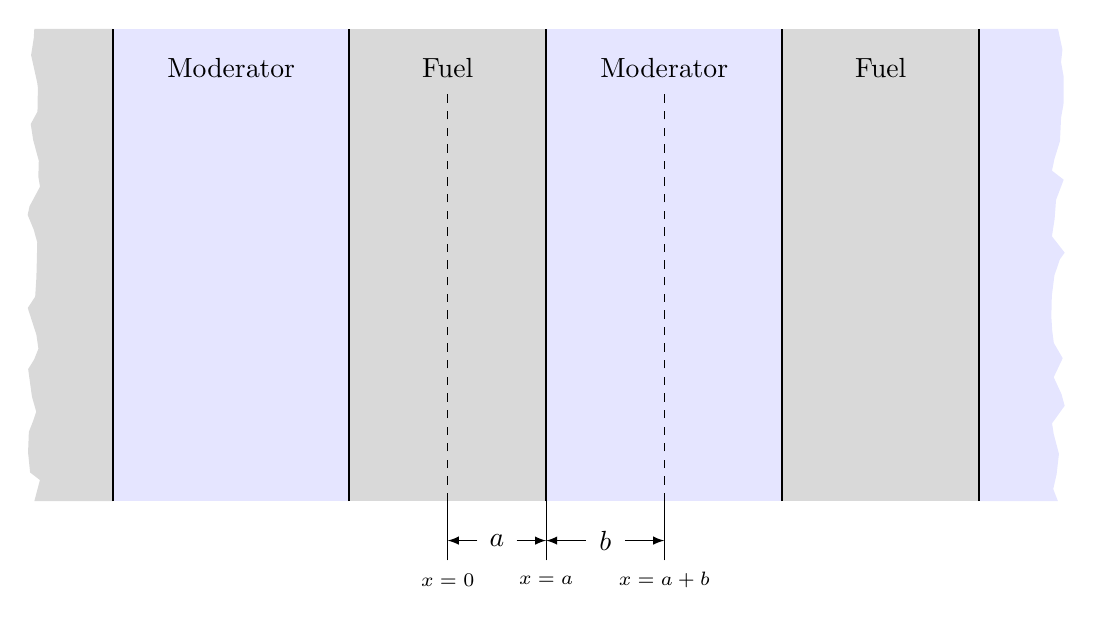
\begin{tikzpicture}
% fuel-moderator boxes
\fill[gray!30, decoration={random steps,segment length=0.2cm}] (-4,-1) decorate{-- (-4,5)} -- (-3,5) -- (-3,-1)-- cycle;
\fill[blue!10] (-3,-1) rectangle (0,5);
\fill[gray!30] (0,-1) rectangle (+2.5,5);
\fill[blue!10] (+2.5,-1) rectangle (+5.5,5);
\fill[gray!30] (+5.5,-1) rectangle (+8.0,5);
\fill[blue!10, decoration={random steps,segment length=0.2cm}] (+9.0,+5.0) decorate{-- (+9.0,-1.0)} -- (+8.0,-1.0) -- (+8.0,+5.0)-- cycle;
%\node at (0,0.5) {\iso{I}{126}{53}};
\draw[thick] (-0,-1) -- (0,5);
\draw[thick] (-3,-1) -- (-3,5);
\draw[thick] (+2.5,-1) -- (+2.5,5);
\draw[thick] (+5.5,-1) -- (+5.5,5);
\draw[thick] (+8.0,-1) -- (+8.0,5);
%
\draw[dashed] (1.25,-1) -- (1.25,4.25);
\draw         (1.25,-1.75) -- (1.25,-1);
\draw         (2.5,-1.75) -- (2.5,-1);
\draw[dashed] (4,-1) -- (4,4.25);
\draw         (4,-1.75) -- (4,-1);
\node at (1.875,-1.5) {$a$};
\draw[-latex] (1.625,-1.5) -- (1.25,-1.5);
\draw[-latex] (2.125,-1.5) -- (2.5,-1.5);
\node at (3.25,-1.5)  {$b$};
\draw[-latex] (3,-1.5) -- (2.5,-1.5);
\draw[-latex] (3.5,-1.5) -- (4,-1.5);
\node at (1.25,-2) {\scriptsize $x = 0$};
\node at (2.5,-2) {\scriptsize $x = a$};
\node at (4,-2) {\scriptsize $x = a+b$};
\node at (-1.5,+4.5) {Moderator};
\node at (+1.25,+4.5) {Fuel};
\node at (+4.0,+4.5) {Moderator};
\node at (+6.75,+4.5) {Fuel};
\end{tikzpicture}
\caption{Illustration of a planar fuel-moderator lattice.}
\label{Fig:ode_planarLattice}
\end{center}
\end{figure}


In this problem the geometry is an infinite 1-D planar lattice of fuel and moderator regions with fuel as region 1 and moderator as region 2 (see Fig.~\ref{Fig:ode_planarLattice}). Since the problem exhibits symmetry we can analyze a single unit cell with symmetry boundary conditions at the reflection planes, namely that the net flow rates of neutrons (neutron current) $J(x)$ are zero across the reflection boundaries. The neutron source $Q_0$ will be spatially constant in region 2, which is the moderator and represents where neutrons slow down into the thermal group. The equations for the fuel and moderator are respectively,
\begin{subequations}
\begin{align}
  &\phi_1''(x) - \frac{1}{L_1^2} \phi_1(x) = 0, \quad 0 \le x \le a; \\*
  &\phi_2''(x) - \frac{1}{L_2^2} \phi_2(x) = -\frac{Q_0}{D_2}, \quad a \le x \le a + b.
\end{align}
\end{subequations}
The boundary and interface conditions are
\begin{subequations}
\begin{align}
  J_1(0) &= 0, \\*
  \phi_1(a) &= \phi_2(a), \\*
  J_1(a) &= J_2(a), \\*
  J_2(a+b) &= 0.
\end{align}
\end{subequations}

The solutions to the differential equations involve real exponentials that we elect to write in terms of the hyperbolic trigonometric functions. This is motivated by the fact that the $\sinh(0) = 0$, which we can use to simplify some of the coefficients. For the moderator region, we also introduce a translation by $a + b$ so we get the $\sinh$ term disappear when we apply the boundary condition. (This ``phase shift'' is simply a redefinition of coefficients. If we apply the sum formulas for the hyperbolic sine and hyperbolic cosine, we can show that the homogeneous solution with and without phase shifts are functionally equivalent.) These are
\begin{subequations}
\begin{align}
  \phi_1(x) &= A_1 \sinh \left( \frac{x}{L_1} \right) + B_1 \cosh \left( \frac{x}{L_1} \right), \\*
  \phi_2(x) &= A_2 \sinh \left( \frac{a+b-x}{L_2} \right) + B_2 \cosh \left( \frac{a+b-x}{L_2} \right) + \frac{Q_0 L_2^2}{D_2}.
\end{align}
\end{subequations}
The net currents are
\begin{subequations}
\begin{align}
  J_1(x) &= -\frac{D_1 A_1}{L_1} \cosh \left( \frac{x}{L_1} \right)     - \frac{D_1 B_1}{L_1} \sinh \left( \frac{x}{L_1} \right), \\*
  J_2(x) &=  \frac{D_2 A_2}{L_2} \cosh \left( \frac{a+b-x}{L_2} \right) + \frac{D_2 B_2}{L_2} \sinh \left( \frac{a+b-x}{L_2} \right) .
\end{align}
\end{subequations}
Applying the symmetry conditions $J_1(0) = 0$ and $J_2(a+b) = 0$, gives the equations
\begin{subequations}
\begin{align}
  -\frac{D_1 A_1}{L_1} &= 0, \\*
   \frac{D_2 A_2}{L_2} &= 0,
\end{align}
which implies that $A_1 = A_2 = 0$. Applying the interface conditions, we obtain
\begin{align}
  &B_1 \cosh \left( \frac{a}{L_1} \right) = B_2 \cosh \left( \frac{b}{L_2} \right) + \frac{Q_0 L_2^2}{D_2}, \\*
  &- \frac{D_1 B_1}{L_1} \sinh \left( \frac{a}{L_1} \right) = \frac{D_2 B_2}{L_2} \sinh \left( \frac{b}{L_2} \right) .
\end{align}
\end{subequations}
We can then write these two equations as a linear system in terms of the coefficients
\begin{align}
  \left[ \begin{array}{c c}
  \cosh \left( \dfrac{a}{L_1} \right)                  & - \cosh \left( \dfrac{b}{L_2} \right) \vspace{0.2cm} \\
  \dfrac{D_1}{L_1} \sinh \left( \dfrac{a}{L_1} \right) & \dfrac{D_2}{L_2} \sinh \left( \dfrac{b}{L_2} \right) \\
  \end{array} \right]
  \left[ \begin{array}{c} B_1 \\ B_2 \\ \end{array} \right] =
  \left[ \begin{array}{c} \dfrac{Q_0 L_2^2}{D_2} \vspace{0.2cm} \\ 0 \end{array} \right] .
\end{align}
Solving this system for the coefficients yields
\begin{subequations}
\begin{align}
  B_1 &= \dfrac{Q_0 L_2^2}{D_2} \left[
         \dfrac{ \dfrac{D_2}{L_2} \sinh \left( \dfrac{b}{L_2} \right) }
               { \dfrac{D_2}{L_2} \cosh \left( \dfrac{a}{L_1} \right) \sinh  \left( \dfrac{b}{L_2} \right)
               + \dfrac{D_1}{L_1} \sinh \left( \dfrac{a}{L_1} \right) \cosh  \left( \dfrac{b}{L_2} \right) } \right], \\*
  B_2 &= -\dfrac{Q_0 L_2^2}{D_2} \left[
         \dfrac{ \dfrac{D_1}{L_1} \sinh \left( \dfrac{a}{L_1} \right) }
               { \dfrac{D_2}{L_2} \cosh \left( \dfrac{a}{L_1} \right) \sinh  \left( \dfrac{b}{L_2} \right)
               + \dfrac{D_1}{L_1} \sinh \left( \dfrac{a}{L_1} \right) \cosh  \left( \dfrac{b}{L_2} \right) } \right].
\end{align}
\end{subequations}
Therefore the solution is
\begin{subequations}
\begin{align}
  \phi_1(x) &= \dfrac{Q_0 L_2^2}{D_2} \left[
         \dfrac{ \dfrac{D_2}{L_2} \sinh \left( \dfrac{b}{L_2} \right) \cosh \left( \dfrac{x}{L_2} \right) }
               { \dfrac{D_2}{L_2} \cosh \left( \dfrac{a}{L_1} \right) \sinh  \left( \dfrac{b}{L_2} \right)
               + \dfrac{D_1}{L_1} \sinh \left( \dfrac{a}{L_1} \right) \cosh  \left( \dfrac{b}{L_2} \right) } \right] , \\*
  \phi_2(x) &= \dfrac{Q_0 L_2^2}{D_2} \left[ 1 -
                \dfrac{ \dfrac{D_1}{L_1} \sinh \left( \dfrac{a}{L_1} \right) \cosh \left( \dfrac{a+b-x}{L_2} \right) }
               { \dfrac{D_2}{L_2} \cosh \left( \dfrac{a}{L_1} \right) \sinh  \left( \dfrac{b}{L_2} \right)
               + \dfrac{D_1}{L_1} \sinh \left( \dfrac{a}{L_1} \right) \cosh  \left( \dfrac{b}{L_2} \right) } \right] .
\end{align}
\end{subequations}

\begin{figure}[tb!]
\begin{center}
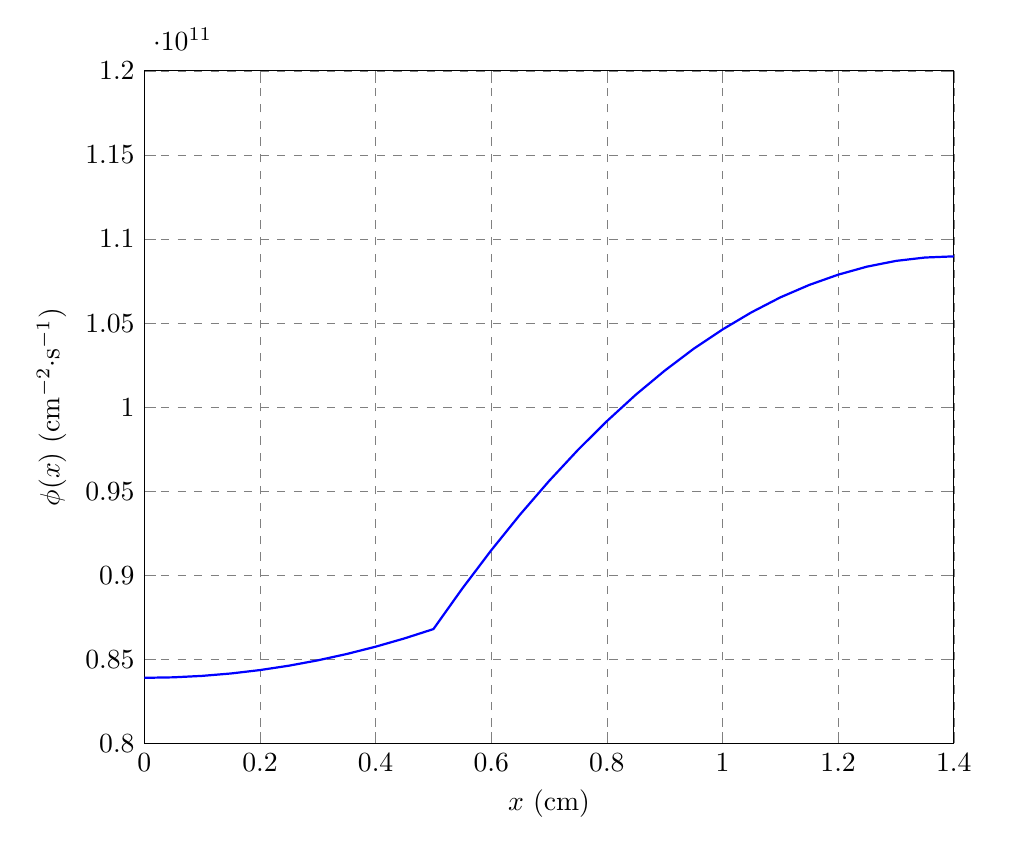
\begin{tikzpicture} \begin{axis}
[scale=1.5,
 xmin=0,    xmax=1.4,
 ymin=8.0e10, ymax=1.2e11,
 grid=major, 
 major grid style={color=gray,line width=0.2pt, dashed},
 xlabel=$x$ (cm),
 ylabel=$\phi(x)$ (cm$^{-2}\cdot$s$^{-1}$),
]

\addplot[line width=0.8pt, color=blue] coordinates {
 (           0 ,  8.3901e+10 )
 (  5.0000e-02 ,  8.3930e+10 )
 (  1.0000e-01 ,  8.4016e+10 )
 (  1.5000e-01 ,  8.4160e+10 )
 (  2.0000e-01 ,  8.4362e+10 )
 (  2.5000e-01 ,  8.4622e+10 )
 (  3.0000e-01 ,  8.4940e+10 )
 (  3.5000e-01 ,  8.5317e+10 )
 (  4.0000e-01 ,  8.5752e+10 )
 (  4.5000e-01 ,  8.6246e+10 )
 (  5.0000e-01 ,  8.6799e+10 )
 (  5.5000e-01 ,  8.9214e+10 )
 (  6.0000e-01 ,  9.1487e+10 )
 (  6.5000e-01 ,  9.3617e+10 )
 (  7.0000e-01 ,  9.5607e+10 )
 (  7.5000e-01 ,  9.7457e+10 )
 (  8.0000e-01 ,  9.9167e+10 )
 (  8.5000e-01 ,  1.0074e+11 )
 (  9.0000e-01 ,  1.0217e+11 )
 (  9.5000e-01 ,  1.0347e+11 )
 (  1.0000e+00 ,  1.0462e+11 )
 (  1.0500e+00 ,  1.0564e+11 )
 (  1.1000e+00 ,  1.0653e+11 )
 (  1.1500e+00 ,  1.0727e+11 )
 (  1.2000e+00 ,  1.0788e+11 )
 (  1.2500e+00 ,  1.0836e+11 )
 (  1.3000e+00 ,  1.0870e+11 )
 (  1.3500e+00 ,  1.0890e+11 )
 (  1.4000e+00 ,  1.0897e+11 )
};
\end{axis}
\end{tikzpicture}
\caption{Neutron scalar flux (path-length rate density) in a planar fuel-moderator lattice.}
 \label{Fig:ode_neutronFluxPlanarLattice}
\end{center}
\end{figure}

The following numbers are representative for a uranium dioxide fuel and light water moderator:
\begin{align}
  a &= 0.5 \text{ cm}, \nonumber \\
  b &= 0.9 \text{ cm}, \nonumber \\
  Q_0 &= 10^{10} \text{ neutrons$\cdot$cm$^{-3}$$\cdot$s$^{-1}$}, \nonumber \\
  D_1 &= 0.615 \text{ cm}, \nonumber \\
  D_2 &= 0.144 \text{ cm}, \nonumber \\
  L_1 &= 1.908 \text{ cm}, \nonumber \\
  L_2 &= 2.685 \text{ cm}. \nonumber
\end{align}
Using those numbers the scalar flux is plotted in Fig.~\ref{Fig:ode_neutronFluxPlanarLattice}. The thermal neutron scalar flux is highest in the moderator region on the right, as this is where the neutrons thermalize. The scalar flux falls as the field gets closer to the fuel as neutrons that enter the fuel tend to be absorbed (some of these absorptions cause fission) and therefore fewer neutrons exit the fuel than exit. As one may expect, the minimum neutron scalar flux is at the center of the fuel.

\subsection{Example: Point Source in an Infinite Medium}

Now that we have done a few examples in 1-D Cartesian coordinates, we should explore the curvilinear coordinates. The next example will consider the case of an isotropic point source that we take to be at the origin within an infinite medium. Because neutrons are emerging from this source with equal probability in all directions in a spherically symmetric manner, it makes the most sense to analyze this problem in spherical geometry.

If we take the source to emit $Q_0$ neutrons per unit time at the origin, the neutron diffusion equation is then
\begin{subequations}
\begin{align}
  \frac{1}{r^2} \frac{d}{dr} \left( r^2 \frac{d\phi}{dr} \right) - \frac{1}{L^2} \phi(r) = -\frac{Q_0}{4\pi D r^2} \delta(r).
\end{align}
Similar to the planar source, we have an infinite value for the source at an infinitesimal location. In this case it is at a single point as opposed to distributed over an infinite planar surface. The boundary condition here states that the net flow of across a vanishingly small spherical surface centered about the origin is equal to the source rate. Additionally, since the domain extends to infinity, we need to ensure the scalar flux stays finite as the radial coordinate goes to infinity---there is no such restriction at the origin because there is a point source that theoretically has infinite density (but finite intensity). The boundary conditions are then,
\begin{align}
  &\lim_{r \rightarrow 0} 4\pi r^2 J(r) = Q_0, \\
  &\lim_{r \rightarrow \infty} \phi(r) < \infty.
\end{align}
\end{subequations}

This first boundary condition converts the inhomogeneous equation into a homogeneous equation. Since the domain extends to infinity, this motivates us to select the exponential form of the solution from Eq.~\eqref{Eq:neutronics_diffusionHomogeneous_1DPlanarExponential}:
\begin{align}
  \phi(r) &= \frac{A}{r} e^{-r/L} + \frac{B}{r} e^{r/L}.
\end{align}
From the condition that the scalar flux must be finite for large $r$, we see that $B = 0$. To apply our boundary condition at the origin, we calculate the net current,
\begin{align}
  J(r) = -D\frac{d\phi}{dr} = \frac{DA}{L r^2} ( L + r ) e^{-r/L} .
\end{align}
Applying the boundary condition, we get
\begin{align}
  \lim_{r \rightarrow 0} 4 \pi r^2  J(r) =  \lim_{r \rightarrow 0} \frac{4\pi DA}{L} ( L + r ) e^{-r/L} = 4 \pi D A = Q_0 .
\end{align}
Therefore,
\begin{align}
  A = \frac{ Q_0 }{ 4\pi D },
\end{align}
and the solution is
\begin{align} \label{Eq:neutronics_diffusionScalarFlux_IsotropicPointSource}
  \phi(r) = \frac{ Q_0 }{ 4 \pi D r } e^{-r/L} .
\end{align}

\subsection{Diffusion Migration Distance} \label{Sec:neutronics_DiffusionMigrationDistance}

The concepts of the diffusion coefficient and diffusion length are convenient to work with mathematically, but their physical meaning is not entirely clear. Fortunately, we can relate these quantities to the root-mean-squared distance neutrons travel before absorption using the result for the scalar flux distribution from an isotropic point source in Eq.~\eqref{Eq:neutronics_diffusionScalarFlux_IsotropicPointSource}. We can then take this further and arrive at some conclusions about the validity of the neutron diffusion equation.

The probability that a neutron will be absorbed in a spherical shell between $r$ and $r + dr$ having volume $4\pi r^2 dr$ is
\begin{align}
  p(r) dr 
  &= \frac{\text{rate neutrons are absorbed between $r$ and $r + dr$}}{\text{rate neutrons are produced from the source}} \nonumber \\
  &= \frac{ \Sigma_a \phi(r) ( 4\pi r^2 ) dr }{ Q_0 } \nonumber \\
  &= \frac{ ( \Sigma_a Q_0 /D ) r e^{-r/L} }{ Q_0 } dr \nonumber \\
  &= \frac{r}{L^2} e^{-r/L} dr .
\end{align}
Here we used the definition of the diffusion length $L^2 = D/\Sigma_a$.

Given the probability density function for the distance to absorption $p(r)$, we can calculate moments of travel. Here, we compute the mean-squared distance as
\begin{align}
  \overline{r^2} = \int_0^\infty r^2 p(r) dr = 6 L^2.
\end{align}
If we take the square root of both sides we can relate the diffusion length $L$ to the root-mean-squared distance as
\begin{align}
  \sqrt{ \overline{r^2} } = \sqrt{6} L .
\end{align}
So the diffusion length is the root-mean-squared distance divided by a factor of $\sqrt{6}$. (In one-speed problems, the diffusion length $L$ as the migration distance and $L^2$ as the migration area. More commonly, however, the concept of migration is applied in the context of fast and thermal groups.)

Given that we know the solution for the point source, we can generalize this for an arbitrary source distribution in an infinite medium provided that we can obtain the scalar flux distribution. The diffusion length in the general case is
\begin{align}
  L^2 = \frac{1}{6} \overline{r^2}= \dfrac{ \displaystyle\int r^2 \phi(\pos) dV }{ \displaystyle\int \phi(\pos) dV } ,
\end{align}
where the integrals are taken over all space.

A bit of digression before we look at the applicability of diffusion theory. An application of this root-mean-squared distance is that it can be generalized to include energy dependence as being how far a neutron travels before being absorbed or slows down to a particular kinetic energy (special considerations are required for upscatter). The root-mean-squared distance are sometimes used to find diffusion coefficients as an alternative to the one obtained from the outscatter approximation. It has been shown that this more physical diffusion coefficient when applied to slowing down in hydrogenous media like water give answers that are more representative of the neutron transport solution with energy dependence.

Back on topic, we claimed earlier that diffusion theory is valid when there is medium is dominated by scattering. This is based on the argument that scattering washes out the directionality of the angular flux. Now that we are armed with the diffusion migration distance. 

In the limit of no scattering, we have a purely absorbing transport problem. The neutron scalar flux from a point source then falls off as an inverse square law with exponential attenuation:
\begin{align}
  \phi_u(r) = \frac{Q_0}{4\pi r^2} e^{-\Sigma_t r} = \frac{ Q_0 }{ 4\pi r^2 } e^{-r/\lambda} .
\end{align}
Here the $u$ subscript means ``uncollided'', as any neutron in the limiting case of a pure absorbing that experiences a collision is absorbed and therefore lost. We also write the mean-free path here as $\lambda = 1/\Sigma_t$. Note that this contrasts with the diffusion problem, where the scalar flux falls off as $1/r$ as opposed to $1/r^2$. This difference in the geometric rate of decrease is because in diffusion theory, we require that most neutrons that undergo collisions survive via the scattering process, whereas in the extreme case of no scattering (pure absorption) these surviving neutrons are absent.

Given the uncollided flux distribution, we can compute the mean-square distance for uncollided neutrons from a point source using similar reasoning as before. The probability that a neutron from the source experiences its first collision in some spherical shell between $r$ and $r + dr$ is
\begin{align}
  p(r) dr = \dfrac{ \Sigma_t \left[ \dfrac{Q_0}{4\pi r^2} e^{-\Sigma_t r} \right] 4\pi r^2 dr }{ Q_0 }
  = \frac{1}{\lambda} e^{-r/\lambda} dr. 
\end{align}
The mean-squared distance for uncollided neutrons is
\begin{align}
  \overline{r_u^2} = \int_0^\infty r^2 p(r) dr = \int_0^\infty \frac{r^2}{\lambda} e^{-r/\lambda} dr = 2 \lambda^2 .
\end{align}
Therefore, the root-mean-squared distance an uncollided neutron travels is
\begin{align}
  \sqrt{ \overline{r_u^2} } = \sqrt{2} \lambda \approx 0.71 \lambda.
\end{align}

We can now express the diffusion migration distance in terms of the mean-free path. If we assume scattering is isotropic and we denote probability of scattering as $c = \Sigma_s/\Sigma_t$, we have that the square of the diffusion length is
\begin{align}
  L^2 = \frac{D}{\Sigma_a} = \frac{1}{3 \Sigma_t} \frac{1}{(1-c)\Sigma_t} = \frac{1}{3(1-c) \Sigma_t^2} = \frac{ \lambda^2 }{ 3 (1-c) } .
\end{align}
The mean-squared distance in terms of the mean-free path is then
\begin{align}
   \overline{r^2} = 6 L^2 = \frac{ 2 \lambda^2 }{ 1 - c } = \frac{ r_u^2 }{ 1 - c }.
\end{align}

For diffusion theory to be satisfactory, we require that the diffusion migration distance (root-mean-squared distance to absorption) be substantially greater than the root-mean-squared distance between neutron collisions:
\begin{align}
  \sqrt{ \frac{  \overline{r^2} }{  \overline{r_u^2} } } = \frac{1}{\sqrt{ 1 - c } } \gg 1.
\end{align}
Clearly, values of the scattering probability $c$ that are closer to one satisfy this condition. If $c = 0.75$, then we have that diffusion migration distance is twice the root-mean-squared distance between neutron collisions. If the scattering ratio is much less than 0.75, then we expect transport effects to dominate and diffusion theory to be a very questionable approximation.

\subsection{Example: Infinite Cylinder with a Constant Source}

In this example we will explore solutions in 1-D cylindrical geometry. Here we have a uniform source of intensity $Q_0$ within a bare cylinder of radius $R$ that is infinite in extent. The neutron diffusion equation is
\begin{subequations}
\begin{align}
  \frac{1}{r} \frac{d}{dr} \left( r \frac{d\phi}{dr} \right) - \frac{1}{L^2} \phi(r) = -\frac{Q_0}{D} .
\end{align}
For the boundary conditions, we require that the scalar flux remains finite at the origin and that there is no inward partial current at the end of the cylinder. This is
\begin{align}
  &\lim_{r \rightarrow 0} \phi(r) < 0, \\
  &J^-(R) = 0.
\end{align}
\end{subequations}
The homogeneous solution is in terms of the modified Bessel functions as in Eq.~\eqref{Eq:neutronics_diffusionHomogeneous_1DCylindricalModifiedBessel}. For the particular solution, since our inhomogeneous source is a constant, we expect that it too is constant. We then have for the solution,
\begin{align}
  \phi(r) = A I_0(r/L) + B K_0(r/L) + \frac{Q_0 L^2}{D} .
\end{align}
Since $K_0(r/L)$ diverges for $r \rightarrow 0$, we require that $B = 0$. We calculate the inward partial current as
\begin{align}
  J^-(R) = \frac{1}{4} \left[ A I_0(R/L) + \frac{Q_0 L^2}{D} \right] + \frac{D}{2} \left[ \frac{A}{L} I_1(R/L) \right] = 0.
\end{align}
Solving for $A$ we get
\begin{align}
  A = -\frac{Q_0 L^2}{D} \bigg[ I_0(R/L) + ( 2D / L ) I_1(R/L) \bigg]^{-1} .
\end{align}
Plugging this in, the scalar flux is then
\begin{align}
  \phi(r) = \frac{ Q_0 L^2 }{ D } \left[ 1 - \frac{ I_0(r/L) }{ I_0(R/L) + (2D/L) I_1(R/L) } \right] .
\end{align}

%%%%%%%%%%%%%%%%%%%%%%%%%%%%%%%%%%%%%%%%%%%%%%%%%%%%%%%%%%%%%%%%%%%%%%%%%%%%%%%%
\section{Green's Function Method}

Solving neutron diffusion problems in two and three spatial dimensions by hand is rather difficult because we must now solve a partial differential equation as opposed to an ordinary one. While in practice we often resort to numerical methods, there are a few cases for which we can readily obtain an analytical solutions using techniques such as Green's functions, separation of variables, or by employing Fourier transforms. In this section, we will briefly discuss the Green's function, which is a way to take the solutions for the isotropic planar and point sources and formulate the solution of a general neutron diffusion problem in a infinite, homogeneous medium as an integral. The Green's function is particularly useful when we want to know localized information about the problem such as the scalar flux in a detector within a system.

Some readers may not be familiar with Green's functions, so we will give a quick overview. The Green's function is a mathematical tool that gives the resulting field described by a linear differential equation from of an inhomogeneous source at a point. Here the key is that the differential equation is linear. In this case, the solution for a field arising from two point sources is the sum or superposition of the solutions from the individual point sources. It reasons then that if we add the contributions from a large number of point sources approximating a spatially distributed inhomogeneous source, we would get an approximation of a solution. In the limit of an infinite number of point sources, we get the integral over a continuous distribution.

Now we should add some mathematical precision to this. The Green's function $G(x,x')$ for our diffusion problem satisfies the following differential equation:
\begin{align}
  \nabla^2 G(\pos,\pos') - \frac{1}{L^2} G(\pos,\pos') = -\frac{1}{D} \delta(\pos - \pos') .
\end{align}
Here $\delta(\pos - \pos')$ is the Dirac delta function. In 1-D this is simply $\delta(x - x')$. In 3-D, we take this as the product of the Dirac delta functions to localize the source:
\begin{align}
   \delta(\pos - \pos') = \delta( x - x' ) \delta( y - y' ) \delta( z - z' ).
\end{align}
The solution to the scalar flux is the volume integral
\begin{align}
  \phi(\pos) = \int Q(\pos') G(\pos,\pos') dV',
\end{align}
where $dV'$ is a differential volume point containing the source and the integrals ``sweeps out'' all points in space giving the contribution from all source locations $\pos'$ to a point of interest $\pos$. In this, we get the solution of the scalar flux at a single point $\pos$, but we can repeat taking the integral at any number of points. 

It turns out that the Green's functions follow from directly from the planar and isotropic point source solutions. For 1-D slab geometry that is infinite and uniform, we use Eq.~\eqref{Eq:neutronics_diffusionScalarFlux_PlanarSource} to get
\begin{align} \label{Eq:neutronics_diffusionGreensFunction_PlanarSource}
  G(x,x') = \frac{ L }{ 2 D } e^{-|x-x'|/L} .
\end{align}
For 3-D media that are infinite and uniform, we use the solution for the isotropic point source from Eq.~\eqref{Eq:neutronics_diffusionScalarFlux_IsotropicPointSource} to obtain
\begin{align} \label{Eq:neutronics_diffusionGreensFunction_IsotropicPointSource}
  G(\pos,\pos')  = \frac{ e^{-|\pos - \pos'|/L}  }{ 4 \pi D |\pos - \pos'| }  .
\end{align}
Here $| \pos - \pos' |$ is the distance between the source location $\pos'$ that we are integrating over and the point of interest $\pos$.

Again, both of these only apply to infinite media that have no spatial variation. There are techniques that can extend the Green's function methods to finite media such as the method of images. We will not pursue these ideas further here and instead move onto different techniques that are useful for analyzing multiplying media found within nuclear reactors.

%%%%%%%%%%%%%%%%%%%%%%%%%%%%%%%%%%%%%%%%%%%%%%%%%%%%%%%%%%%%%%%%%%%%%%%%%%%%%%%%
\section{Neutron Diffusion in Nuclear Reactors}

Now that we have gone over how to solve problems for nonmultiplying media, we will move toward our goal of applying neutron diffusion to nuclear reactors. Here we will make the assumption that all neutrons travel with some representative speed. This will permit analytical solutions to develop an intuition. Of course, actual analysis of reactors requires the consideration of energy dependence, and we will add this extra complication later in this chapter.

\subsection{Time-Dependent Neutron Diffusion in a 1-D Slab} \label{Sec:neutronics_timeDependentDiffusion_1DSlab}

To begin our analysis, we consider the time-dependent neutron diffusion equation in 1-D slab geometry with uniform material properties and no internal source:
\begin{subequations}
\begin{align}
  \frac{1}{v} \dho{}{t} \phi(x,t) - D \frac{\partial^2}{\partial x^2} \phi(x,t) + \Sigma_a \phi(x,t) = \nu \Sigma_f \phi(x,t),
\end{align}
on the domain $0 \le x \le a$. Here we specify some initial condition on the scalar flux,
\begin{align}
  \phi(x,0) = \phi_0(x).
\end{align}
Since there is no internal source, the neutrons will migrate over time via the diffusion process. We will see that over long times, the neutron population will either grow or decay exponentially depending on the balance of losses from leakage and absorption and the gains from fission. We require two boundary conditions to solve this problem. The correct boundary conditions are the Marshak boundary conditions, but these will make our analysis quite complicated. Using an extrapolated boundary condition will simplify this considerably. If we assume that the reactor is large such that size is much greater than the extrapolation distance $\delta$, we can, with very little error, take the scalar flux to be zero at the edges:
\begin{align}
  \phi(0) &= 0, \\
  \phi(a) &= 0.
\end{align}
\end{subequations}
Note that the choices here of 1-D slab geometry and zero-flux boundary conditions do not impact the overall conclusions. What we show in this section will apply to the general case and we can even extrapolate in a conceptual sense to the behavior with energy dependence.

Since this is a partial differential equation, the previous techniques we used are not applicable. Instead, we will use the method of separation of variables. To begin, we rearrange the equation by dividing by the diffusion coefficient and move the absorption term to the right-hand side
\begin{align}
  \frac{1}{v D} \dho{\phi}{t} - \dhotwo{\phi}{x} = \frac{ \nu \Sigma_f - \Sigma_a }{ D } \phi(x,t) .
\end{align}
We then assume the solution is separable of the form
\begin{align}
  \phi(x,t) = X(x) T(t) ,
\end{align}
insert this into the differential equation, and divide by $\phi(x,t)$ to obtain
\begin{align}
  \frac{1}{v D T} \frac{dT}{dt} - \frac{1}{X} \frac{d^2 X}{dx^2} = \frac{ \nu \Sigma_f - \Sigma_a }{ D } .
\end{align}
We now have an equation where the right-hand side is equal to a constant and the time and space terms are only dependent on the time and space variables. Since the first term of the left can only a function of time and the second term a function of space, the only way for them to add up to a constant is for both of their functional dependences on time and space respectively to also be constant.

There are three possibilities for the constant: positive, negative, or zero. It turns out that only the negative constant yields a solution that simultaneously satisfies the boundary conditions while yielding a non-trivial solution. We will leave checking this is indeed the case as an exercise here and state that
\begin{subequations}
\begin{align}
  \frac{1}{vD T} \frac{dT}{dt} &= \frac{ \nu \Sigma_f - \Sigma_a }{ D } - B^2, \\
  \frac{1}{X} \frac{d^2 X}{dx^2} &= -B^2 .
\end{align}
\end{subequations}
Here $B^2$ is some constant for which we will find valid solutions. (Later on, we will call this coefficient the buckling, as it follows similar mathematics to structural mechanics, but otherwise has no physical connection to the phenomena in nuclear reactors.)

The solution for the spatial function $X$ can be expressed using the trigonometric functions:
\begin{align}
  X(x) = A \sin ( Bx ) + C \cos ( Bx ) .
\end{align}
Applying the boundary conditions $X(0)$ gives
\begin{align}
  X(0) = A \sin( 0 ) + C \cos( 0 ) = C = 0. \nonumber
\end{align}
Doing the same at $x = a$ gives the following,
\begin{align}
  X(a) = A \sin( Ba ) = 0.
\end{align}
This can only be true when $Ba$ is a positive integer multiple of $\pi$. The case where it is zero is the trivial solution, which means no neutrons in the reactor, which is pretty boring to be honest. The case of negative integer multiplies of $\pi$ yield the same result with different coefficients and provide no unique information. To summarize, we have
\begin{subequations}
\begin{align}
  C &= 0, \\
  A &= \frac{n\pi}{a}, \quad n = 1, 2, 3, \ldots
\end{align}
\end{subequations}
Therefore, we have obtained infinitely many solutions to the $X$ equation. The general solution of this is therefore a linear combination of all possible solutions:
\begin{align}
  X(x) = \sum_{n=1}^\infty A_n \sin \left( \frac{ n \pi x }{ a } \right) .
\end{align}
Each term in the summation has a different constant coefficient.

The time term is obtained in a similar process. Since it is s first-order ordinary differential equation, we know the solution should be an exponential. We get
\begin{align}
  T(t) = K \exp \left[ \left( \nu \Sigma_f - \Sigma_a - \left( \frac{n \pi}{a} \right)^2 D \right) vt \right] .
\end{align}
We will see shortly that the values within the exponential will have a significant impact on the time-evolution and criticality of the system. 

Multiplying the space and time terms together and combining constants gives the solution for 1-D transient neutron diffusion
\begin{align}
  \phi(x,t) = \sum_{n=1}^\infty A_n \sin \left( \frac{ n \pi x }{ a } \right) \exp \left[ \left( \nu \Sigma_f - \Sigma_a - \left( \frac{n \pi}{a} \right)^2 D \right) v t \right]  . \label{Eq:neutronics_timeDependentScalarFlux_1DSlabDiffusion}
\end{align}

We will now study the term in the exponential and its impact on the long-time behavior. We have
\begin{align}
   \nu \Sigma_f - \Sigma_a - \left( \frac{n \pi}{a} \right)^2 D \nonumber
\end{align}
which gives the production coefficient for fission, the loss coefficient for absorption, and a third term that is a loss term proportional to the neutron diffusion coefficient divided by the length of the reactor squared. The last term describes the physical phenomenon of leakage of neutrons from the system. Note that the least negative of these terms has $n = 1$ and we can deduce that it will be the term that dominates over the others. 

We can state that if
\begin{align}
  \nu \Sigma_f = \Sigma_a + \left( \frac{\pi}{a} \right)^2 D  \nonumber
\end{align}
then the largest exponential term will be zero with all others negative. This is referred to as a \emph{critical} reactor and implies that after long times the neutron distribution will reach a steady state sine wave distribution. The case where
\begin{align}
  \nu \Sigma_f < \Sigma_a + \left( \frac{\pi}{a} \right)^2 D  \nonumber
\end{align}
corresponds to a \emph{subcritical} reactor. This means that the neutron population will reach a sine wave that is decaying exponentially in time. (This behavior is to what one gets for a time-dependent heat conduction problem.) Finally, we have the case where
\begin{align}
  \nu \Sigma_f > \Sigma_a + \left( \frac{\pi}{a} \right)^2 D . \nonumber
\end{align}
This is the \emph{supercritical} configuration, which corresponds to a long time solution that is a sine wave that grows exponentially with time. 

There is still the task of finding the coefficients. For this, we need to use our initial condition. At time $t = 0$, we have
\begin{align}
  \phi(x,0) = \sum_{n=1}^\infty A_n \sin \left( \frac{ n \pi x }{ a } \right) = \phi_0(x)
\end{align}
Theoretically there are infinitely many of these, but in practice we can often get away with computing the first few and get a reasonable description of the time behavior. To solve for these coefficients, we need to somehow isolate each $A_n$. This can be done using what is called ``Fourier's trick''. The sine and cosine functions are orthogonal and therefore satisfy the following:
\begin{subequations}
\begin{align}
  &\int_0^a \sin\left( \frac{n\pi x}{a} \right) \sin\left( \frac{m\pi x}{a} \right) dx = \frac{a}{2} \delta_{nm}, \\
  &\int_0^a \cos\left( \frac{n\pi x}{a} \right) \sin\left( \frac{m\pi x}{a} \right) dx = \frac{a}{2} \delta_{nm}, \\  
  &\int_0^a \cos\left( \frac{n\pi x}{a} \right) \sin\left( \frac{m\pi x}{a} \right) dx = 0.  
\end{align}
\end{subequations}
?ere $\delta_{nm}$ is the Kronecker delta function that is one when $n = m$ and zero when $n \ne m$.

Armed with this new knowledge, we can obtain a single coefficient by multiplying our initial condition by $\sin(m\pi x/a)$ and integrating over the reactor from $0 \le x \le a$. The orthogonality property will eliminate all the coefficients except for the one we are interested in. This is
\begin{align}
  &\sum_{n=1}^\infty A_n \int_0^a \sin \left( \frac{ n \pi x }{ a } \right) \sin \left( \frac{ m \pi x }{ a } \right) dx = \int_0^a \phi_0(x) \sin \left( \frac{ m \pi x }{ a } \right) dx, \nonumber \\
   &\sum_{n=1}^\infty A_n \frac{a}{2} \delta_{mn} = \int_0^a \phi_0(x) \sin \left( \frac{ m \pi x }{ a } \right) dx, \nonumber \\ 
   &A_m = \frac{2}{a} \int_0^a \phi_0(x) \sin \left( \frac{ m \pi x }{ a } \right) dx.
\end{align}
Since $m$ is an arbitrary index on the last line and $n$ has vanished, we can just replace it with $n$ and we have our coefficient in terms of $n$. Therefore, to find each coefficient $A_n$ we must evaluate an integral over the initial condition times the sine function with a matching spatial frequency (wave number). 

Higher-order coefficients have higher spatial frequencies and are often referred to as the higher harmonics. Because of the exponential terms in time, these higher harmonics will decay away more quickly (or grow in magnitude less quickly) than the lower ones. For long times, we then expect only the lowest order term to remain relevant.

\subsection{Criticality Condition}

In previous section we derived the criticality condition for a bare, 1-D slab reactor. We can write this generally as
\begin{align}
  \nu \Sigma_f = \Sigma_a + B^2 D ,
\end{align}
where $B^2$ is called the \emph{geometric buckling} or sometimes just the buckling. We could repeat our analysis for different geometries, and all that would change is $B^2$. In all cases, this quantity will be inversely proportional to the square of the length scale along a particular dimension. 

If we multiply this expression by the scalar flux, we see that the left-hand side is $\nu \Sigma_f \phi$, the fission neutron production rate, and the first term on the right is $\Sigma_a \phi$, the absorption rate. The quanitty $B^2 D \phi$ can be interpreted as the leakage rate such that
\begin{align}
  B^2 D = 	&\text{ effective leakage ``macroscopic cross section'' for } \nonumber \\
  			&\text{ a bare, homogeneous system.} \nonumber
\end{align}

This makes sense from a units perspective as $B^2$ is inverse area and $D$ has units of length, meaning $B^2 D$ has units of inverse length, which is the same as a macroscopic cross section. Here we use the term ``effective'' for this ``cross section'', because obviously neutrons near the center of the system are less likely to leak out versus neutrons near the boundary. We can think of this then as being for a representative neutron somewhere in the system that experiences average behavior.

Furthermore, this makes sense physically. The geometric buckling $B^2$ is inversely proportional to the length scale of the system. The smaller the system, the larger the value of $B^2$, and the larger the leakage. The diffusion coefficient $D$ is proportional to the diffusion length that is itself related to the distance neutrons migrate before being absorbed. The larger value of $D$ implies that neutrons migrate further and are more likely to reach the boundary and leak out. Therefore $B^2$ gives the impact of geometry on leakage and $D$ gives the impact of the material properties.

We can rewrite our form of the criticality condition by solving for the geometric buckling:
\begin{align}
  B^2 = \frac{ \nu \Sigma_f - \Sigma_a }{ D }.
\end{align}
Sometimes the right-hand side is referred to as the \emph{material buckling}. Therefore, the criticality condition (for a bare system) is achieved when the geometric and material bucklings are in balance.

Of course, we have the task of calculating these for different bare geometries. From our time-dependent analysis, we showed that the steady state solution at criticality is constant in time. Based on this, if we have a critical, bare system, we can write down the general diffusion problem for the spatial distribution or shape function:
\begin{align}
  -D \nabla^2 \phi(\pos) + \Sigma_a \phi(\pos) = \nu \Sigma_f \phi(\pos) .
\end{align}
This can then be expressed in terms of the material buckling and related to the geometric buckling:
\begin{align}
  \nabla^2 \phi(\pos) + \left( \frac{ \nu \Sigma_f - \Sigma_a }{ D } \right) \phi(\pos) = \nabla^2 \phi(\pos) + B^2 \phi(\pos) = 0.
\end{align}

Note that we can write this equation as
\begin{align}
  -\nabla^2 \phi(\pos) = B^2 \phi(\pos) . \nonumber
\end{align}
The $-\nabla^2$ is an operator acting on a function, which is equal to a constant $-B^2$ multiplying that same function. This is the definition of an eigenvalue problem, where $B^2$ is the eigenvalue of the operator $-\nabla^2$. These eigenvalues $B^2$ and corresponding eigenfunctions $\phi(\pos)$ depend on the choice of geometry, which changes the functional form of the Laplacian. The task ahead then is to solve this eigenvalue problem for various bare geometries. 

\subsubsection{1-D Slab}

We already did this one before, but we are going to redefine it slightly. Now the slab will range from $-a \le x \le a$ instead, such that $a$ can is the half-thickness. The reason for this redefinition is the half-thickness is analogous to the radial coordinate we see in cylindrical and spherical coordinates. The equation and zero-flux boundary conditions are
\begin{subequations}
\begin{align}
  &\frac{d^2 \phi}{dx^2} + B^2 \phi(x) = 0, \quad -a \le x \le a, \\
  &\phi(-a) = \phi(a) = 0.
\end{align}
\end{subequations}

Since $B^2$ is a positive number (note that we can generalize the buckling to all cases by allowing $B$ to be imaginary), we expect the solution to follow trigonometric functions or complex exponentials, with the former being a better choice for the purposes here.  Because of the boundary conditions and the symmetry of the problem, we require that the solution follow a cosine shape. Therefore, our shape function is
\begin{subequations}
\begin{align}
  \phi(x) = A \cos\left( \frac{\pi x}{2 a} \right),
\end{align}
and the buckling is
\begin{align}
  B^2 = \left( \frac{\pi}{2a} \right)^2 .
\end{align}
\end{subequations}
This is essentially the same as what we had before, but with a cosine instead of a sine and a factor of one-half in the buckling because the problem has width of $2a$ versus $a$ this time.

Before proceeding, we note that the coefficient $A$ is arbitrary. Since this is an eigenvalue problem, we know that an eigenfunction is unique to within a multiplicative constant, so this should be unsurprising. In practice, $A$ has a physical meaning in that it gives the magnitude of the eigenfunction, which is proportional to the number of fissions and the reactor power. What this says is that the reactor shape function is the same and we are free to adjust the power level. Of course, this is mathematical result and implicitly we neglected the fact that power level impacts temperature, which impacts the cross sections and other material properties. So in reality, we are of course not free to pick an arbitrary power level. However, for the time being we will ignore this fact until much later when we get to reactor feedback and control.

\subsubsection{3-D Box}

Solving the problem in two and three spatial dimensions in Cartesian coordinates follows essentially the same procedure. In both cases, we employ separation of variables to grind out a solution. For the 3-D problem, we have a box with dimensions $-a \le x \le a$, $-b \le y \le b$, and $-c \le z \le c$. The neutron diffusion for the shape function is then
\begin{subequations}
\begin{align}
  &\dhotwo{\phi}{x} + \dhotwo{\phi}{y} + \dhotwo{\phi}{z} + B^2 \phi(x,y,z) = 0, \nonumber \\
  &-a \le x \le a, -b \le y \le b, -c \le z \le c, \\
  &\phi(-a,y,z) = 0, \quad \phi(a,y,z)  = 0, \quad \phi(x,-b,z) = 0, \nonumber \\
  &\phi(x,b,z)  = 0, \quad \phi(x,y,-c) = 0, \quad \phi(x,y,c)  = 0.
\end{align}
\end{subequations}

The solution is
\begin{subequations}
\begin{align}
  \phi(x,y,z) = A \cos\left( \dfrac{\pi x}{2 a} \right) \cos\left( \dfrac{\pi y}{2 b} \right) \cos\left( \dfrac{\pi z}{2 c} \right),
\end{align}
which is simply the product of the 1-D solution along each direction, but with the appropriate coordinates. The buckling is
\begin{align}
  B^2 = \left( \dfrac{\pi}{2a} \right)^2 + \left( \dfrac{\pi}{2b} \right)^2 + \left( \dfrac{\pi}{2c} \right)^2,
\end{align}
\end{subequations}
which is the sum of the bucklings for the 1-D problem, except again using the appropriate coordinates and dimensions.

One observation we can make is that the buckling is higher in 3-D versus the equivalent 1-D problem. This makes physical sense. The larger the buckling, the higher the leakage. For the 1-D case, the problem is uniform and infinite along two of the dimensions, which means there is zero leakage along them. For 3-D, those dimensions have finite thickness and neutrons can leak out along them, leading to an increase in the buckling. Note that both the shape function and buckling reduce to the 1-D problem in the limit that $b \rightarrow \infty$ and $c \rightarrow \infty$. The contributions to the buckling vanish in the limit, and the period of the cosines in $y$ and $z$ become infinite, making them constant.

\subsubsection{Sphere}

The next geometry we consider is the case of a uniform sphere of radius $R$. Because of spherical symmetry, there can be no variation along the polar and azimuthal spatial coordinates. As we saw before, the solution will involve a $1/r$ term, and we will therefore require that the shape function be finite at the origin. The diffusion problem is then
\begin{subequations}
\begin{align}
  &\frac{1}{r^2} \frac{d}{dr} \left( r^2 \frac{d\phi}{dr} \right) + B^2 \phi(r) = 0, \quad 0 \le r \le R, \\
  &\phi(0) < \infty, \quad \phi(R) = 0.
\end{align}
\end{subequations}

The solution to this problem are the sine and cosine functions divided by the radial coordinate $r$. Since $\sin(r)/r$ limits to one at the origin and $\cos(r)/r$ limits to infinity, we therefore require that the solution follow a sine form:
\begin{subequations}
\begin{align}
  \phi(r) = \frac{A}{r} \sin\left( \frac{\pi r}{R} \right) .
\end{align}
The buckling for spherical geometry is then
\begin{align}
 B^2 = \left( \frac{\pi}{R} \right)^2 .
\end{align}
\end{subequations}

\subsubsection{Infinite Cylinder}

Now we will move onto the cylindrical geometries, which are probably the most relevant to realistic nuclear reactor geometries. The first case is where the cylinder has an infinite height, such that there is only variation along the radial coordinate. As with spherical geometry, we require the solution to be finite at the origin. Therefore, the neutron diffusion problem becomes
\begin{subequations}
\begin{align}
  &\frac{1}{r} \frac{d}{dr} \left( r \frac{d\phi}{dr} \right) + B^2 \phi(r) = 0, \quad 0 \le r \le R, \\
  &\phi(0) < \infty, \quad \phi(R) = 0.
\end{align}
\end{subequations}

As with the case for non-multiplying media, none of the standard functions we typically encounter satisfy this differential equation. We saw the nonmultiplying case where the term on $\phi(r)$ is negative, that the solutions are the modified Bessel functions, which are exponential-like in nature. Since $B^2$ is positive, we get a different set of functions, namely the standard \emph{Bessel functions}:
\begin{align}
  \phi(r) = A J_0 \left( Br \right) + B Y_0 \left( B r \right) .
\end{align}
Here $J_0$ is the Bessel function of the first kind and $Y_0$ is the Bessel function of the second kind. 

Some comments are in order here, since these may be unfamiliar to many readers. The standard Bessel functions exhibit a damped oscillatory behavior as $r$ moves away from the origin. This type of behavior is consistently analogous to the Cartesian case: exponentials for negative coefficient and oscillatory for positive coefficient. Furthermore, near the origin, these standard Bessel functions have similar behavior to their modified counterparts $I_0$ and $K_0$: namely we get that $J_0$ is finite and $Y_0$ diverges. Therefore, we require that $B = 0$ in order for the solution to be finite. 

Therefore, for a reactor that is cylindrical, we therefore have for cylindrical geometry that the radial solution follows the Bessel function of the first kind:
\begin{subequations}
\begin{align}
  \phi(r) = A J_0 \left( \frac{\nu_0 r}{R} \right).
\end{align}
The buckling for the infinite cylinder is then
\begin{align}
 B^2 = \left( \frac{\nu_0}{R} \right)^2 .
\end{align}
\end{subequations}
There is an constant here $\nu_0$ that may be unfamiliar to many readers. This is a mathematical constant that corresponds to the first (or zeroth) root of the Bessel function and takes on the value of approximately 2.405. (This is confusingly close to the mean number of neutrons per fission for thermal neutrons on $^{235}$U and should not be confused as such.) In these expressions, $\nu_0$ plays a similar role to $\pi$, such that when we plug in a value of $r = R$, we get $J_0(\nu_0)$, which is zero.

Note that in certain reactor designs such as gas- or molten-salt-cooled pebble-bed modular reactors, the reactor has an annular active core. In this case, we need to include both Bessel functions $J_0(Br)$ and $Y_0(Br)$. Since there needs to be an inner inactive reflector region that the annular active core must be around, this cannot be a simple one-region problem and the techniques in this section really do not apply. Later in this section we consider this type of scenario.
 
\subsubsection{Finite Cylinder}

Of course, there is no such object as an infinite cylinder. While often reactors are quite tall, they are still finite in size and there is variation of the neutron flux in the axial direction that needs to be accounted for. We define our finite cylinder as having a radius $R$ and height $2h$. The diffusion problem is then
\begin{subequations}
\begin{align}
  &\frac{1}{r} \frac{\partial}{\partial r} \left( r \frac{\partial \phi}{\partial r} \right) \dhotwo{\phi}{z} + B^2 \phi(r,z) = 0, \quad 0 \le r \le R, \quad -h \le z \le h, \\
  &\phi(0) < \infty, \quad \phi(R) = 0, \quad \phi(-h) = \phi(h) = 0.
\end{align}
\end{subequations}

This can be solved using separation of variables. The solution to this problem is
\begin{subequations}
\begin{align}
  \phi(r) = A J_0 \left( \frac{\nu_0 r}{R} \right)  \cos\left( \frac{\pi z}{2 h} \right).
\end{align}
The buckling for the finite cylinder is
\begin{align}
 B^2 = \left( \frac{\nu_0}{R} \right)^2 + \left( \frac{\pi}{2h} \right)^2 .
\end{align}
\end{subequations}

This solution is a hybrid of the infinite cylinder and the 1-D slab problem. The shape function is the product of the two solutions, which is perhaps not too surprising given that we can use separation of variables to solve the problem. The buckling is the sum of the two. As with the box compared to the slab, the buckling with the finite cylinder is greater than the infinite cylinder. This makes sense because in this case neutrons can leak out on the top and bottom.

\subsubsection{Boundary Condition Extrapolation Correction}

One issue with these results is that we assumed a zero-flux boundary condition. This is inconsistent with the Marshak boundary conditions of the diffusion problem and certainly not consistent with transport-based results. Directly applying the Marshak boundary conditions would yield a problem that is far more complicated, requiring solutions of transcendental equations. While we will get a healthy dose of this in finite media, we can thankfully simplify matters here by using our earlier results for the extrapolation distance.

We can correct for the true boundary condition by replacing all of the spatial variables in the buckling and shape functions with that length plus the extrapolation distance $\delta$. For example, the radius of a sphere in all of these expressions becomes:
\begin{align}
  \tilde{R} = R + \delta .
\end{align}
In terms of the choice of $\delta$, we can use either the Marshak extrapolation of $\delta = 2/( 3 \Sigma_{tr})$ or the more accurate Mile extrapolation $\delta = 0.7104/\Sigma_{tr}$. Note that the physical geometry still has the standard dimension, not the extrapolated one.

\subsubsection{Summary}

We summarize the results of these calculations along with the flux shapes in Table~\ref{Table:neutronics_BucklingDifferentGeometries}. Again the tilde denotes the spatial dimension plus the extrapolation distance $\delta$. Note that the box widths are $2a$, $2b$, and $2c$, and the height of the cylinder if $2h$. This is done so that the extrapolation distance is applied to both ends.

\begin{table}[tb!]
\caption{Summary of Geometric Bucklings and Flux Shapes for Various Geometries}
\begin{center}
\begin{tabular}{|c|c|c|} \hline
  Geometry 			& Buckling $B^2$ 						& Flux Shape $\phi(\pos)$ 						\\ \hline
  1-D Slab			& $\left( \dfrac{\pi}{2\tilde{a}} \right)^2$	& $\cos\left( \dfrac{\pi x}{2 \tilde{a}} \right)$ 	\\ \hline
  3-D Box			& $\left( \dfrac{\pi}{2\tilde{a}} \right)^2 + \left( \dfrac{\pi}{2\tilde{b}} \right)^2 + \left( \dfrac{\pi}{2\tilde{c}} \right)^2$ 
					& $\cos\left( \dfrac{\pi x}{2 \tilde{a}} \right) \cos\left( \dfrac{\pi y}{2 \tilde{b}} \right) \cos\left( \dfrac{\pi z}{2 \tilde{c}} \right)$ \\ \hline
  Sphere			& $\left( \dfrac{\pi}{\tilde{R}} \right)^2$		& $\dfrac{1}{r} \sin\left( \dfrac{\pi r}{\tilde{R}} \right)$ \\ \hline
  Infinite Cylinder	& $\left( \dfrac{\nu_0}{\tilde{R}} \right)^2$	& $J_0 \left( \dfrac{\nu_0 r}{\tilde{R}} \right)$ \\ \hline
  Finite Cylinder	& $\left( \dfrac{\nu_0}{\tilde{R}} \right)^2 + \left( \dfrac{\pi}{2\tilde{h}} \right)^2$
					& $J_0 \left( \dfrac{\nu_0 r}{\tilde{R}} \right) \cos\left( \dfrac{\pi z}{2\tilde{h}} \right)$ \\ \hline
\end{tabular}
\end{center}
\label{Table:neutronics_BucklingDifferentGeometries}
\end{table}%

\subsection{Effective Multiplication Factor} \label{Sec:neutronics_oneSpeedEffectiveMultipicationFactor}

We have defined the condition for nuclear criticality, which allows for finding a combination of material and geometric properties that would render a multiplying system critical. We can extend this definition further by defining an index for criticality $k$ that we call the \emph{effective multiplication factor}. At criticality, the ratio of the rate neutrons are produced from fission must balance the rate they are removed from absorption (which includes fission) or leakage. 

To begin, we return to the one-speed neutron diffusion problem:
\begin{align}
  \frac{1}{v} \dho{\phi}{t} - \nabla \cdot D(\pos)  \nabla \phi(\pos) + \Sigma_a(\pos) \phi(\pos) = \nu \Sigma_f(\pos) \phi(\pos) + Q(\pos). \nonumber
\end{align}
In an operating nuclear reactor, we expect that (a) the neutron is in steady state such that the time derivative is zero, and (b) the neutron population at any point in time should predominantly come from fission as opposed to any internal sources, i.e., from start-up sources, spontaneous fission, and cosmic rays and $Q(\pos) \approx 0$, and external sources. These two conditions can only be simultaneously true when the reactor is precisely in its critical configuration. For any non-critical configuration, the equation 
\begin{align}
   - \nabla \cdot D(\pos)  \nabla \phi(\pos) + \Sigma_a(\pos) \phi(\pos) = \nu \Sigma_f(\pos) \phi(\pos)  \nonumber
\end{align}
would not have a valid solution. We can fix this by introducing a mathematical adjustment factor $1/k$ onto the fission term to arrive at what is called the $k$-eigenvalue form of the neutron diffusion equation:
\begin{align}
   - \nabla \cdot  D(\pos) \nabla \phi(\pos) + \Sigma_a(\pos) \phi(\pos) = \frac{1}{k} \nu \Sigma_f(\pos) \phi(\pos) .
\end{align}
(It is not immediately apparent this is an eigenvalue problem. When we put in energy dependence later on in this chapter, we will formally show this. For now, we will keep things simple and just go with it.)  Here $k$ is the index for criticality and is defined to be the factor that globally adjusts the intensity of fission source to balance the losses. A good part of reactor analysis involves solving for $k$ and the associated shape function $\phi(\pos)$.

At the moment this a bit abstract, so we will return to the case where the material properties are uniform over the entire problem so that we can factor the diffusion coefficient out of the Laplacian operator. This enables us to apply separation of variables and arrive at our buckling eigenvalue problem,
\begin{align}
  \nabla^2 \phi(\pos) = -B^2 \phi(\pos) .
\end{align}
Replacing the Laplacian operator with the right-hand side eliminates all the derivatives, allowing us to algebraically solve for the multiplication factor:
\begin{align}
  k = \frac{ \nu \Sigma_f }{ \Sigma_a + B^2 D } .
\end{align}
It should hopefully be apparent that when $k$ is greater than one, the production of neutrons from fission would exceed the rate they are lost, we call this condition \emph{supercritical}. Based on our time-dependent analysis, we would expect that for long times the neutron population would grow exponentially. (The short-time behavior depends on the initial condition.) Conversely, when $k$ is less than one, the losses would exceed the gains, and we would expect the long-time trend of the neutron population to decay exponentially. We call this condition \emph{subcritical}. To summarize:
\begin{align}
  &k < 1, \quad \text{ subcritical}, \nonumber \\
  &k = 1, \quad \text{ critical}, \nonumber \\
  &k > 1, \quad \text{ supercritical}. \nonumber
\end{align}
This idea applies to the general neutron diffusion and transport problem as well.

We can rewrite this for the one-speed case to get more insight into the physics. From the definition of the diffusion length, we have
\begin{align}
  D = \Sigma_a L^2 . \nonumber
\end{align}
Plugging this in and factoring out the absorption cross section we have
\begin{align}
  k = \frac{ \nu \Sigma_f }{ \Sigma_a } \frac{1}{ 1 + B^2 L^2 } .
\end{align}
If we analyze this expression, the ratio $\Sigma_f / \Sigma_a$ is the probability that a neutron has fission given conditioned on that it was absorbed. (Again, absorption includes fission.) 

The interpretation of the factor $1/(1 + B^2 L^2)$ is a bit less obvious. Since $B^2 L^2$ is obviously positive, we deduce that the denominator is greater than or equal to one. Therefore, this factor ranges between zero and one and could be interpreted as a probability. Since $B^2$ quantifies the geometric effects of leakage in units of per area, with $L^2$ being a measure of the squared migration length or migration area, we can interpret $B^2 L^2$ as dimensionless factor that quantifies the intensity of leakage. The limit of $B^2 L^2 = 0$ implies the geometry is infinite, and the factor is one. The limiting case of $B^2 L^2$ implies infinite leakage intensity so that all neutrons would leak out with probability 1. Therefore, we can interpret this as the non-leakage probability
\begin{align}
  P_{NL} = \text{ (one-speed) non-leakage probability} =  \frac{1}{ 1 + B^2 L^2 } .
\end{align}
Because for the one-speed problem neutrons can only either be absorbed or leak out, the non-leakage probability is also the probability that a neutron is absorbed.

Putting this together, for the one-speed problem, we can express the effective multiplication factor for a one-speed problem as
\begin{align}
   k = 		\left( \parbox{6em}{mean number of neutrons produced per fission} \right)
   \cdot	\left( \parbox{7em}{probability that a neutron undergoes fission if it is absorbed} \right)
   \cdot	\left( \parbox{8.5em}{probability that a neutron does not leak out and is therefore absorbed} \right) . \nonumber
\end{align}
This might be starting to feel like the six-factor formula, except here we only have two terms. Once we get to considering energy dependence, we will revisit this notion and connect it to diffusion theory and the effective multiplication factor.

From this reasoning, we can define the effective multiplication factor for an infinite system where there is no leakage by setting $P_{NL} = 1$. We call this $k$-infinity, and for one-speed we have
\begin{align}
  k_\infty = \frac{ \nu \Sigma_f }{ \Sigma_a } .
\end{align}
This represents the maximum possible effective multiplication factor for a given set of material properties in any geometry. Consequently, if $k_\infty < 1$ of a particular material, then it is impossible to build a reactor out of it without changing the material composition.

\subsection{Reflected Reactors}

In the previous analysis, we require that the reactor be bare, i.e., not surrounded by anything. In practice, we often surround a reactor by a material called a reflector. The purpose of the reflector is to have some of the neutrons that would have otherwise leaked out the reactor scatter within the reflector and migrate back in. The net effect of this is that the addition of a reflector lowers the amount of fissile material required to achieve criticality. For obvious reasons then, we should figure out a means to analyze this scenario.

A reflected system requires an analysis of a two-region diffusion problem. As we saw for the non-multiplying case, having multiple regions often leads to algebra that can become quite tedious. In turns out, our criticality condition for a reflected geometry is likewise not simple as with the bare case. Rather, the analysis inevitably results in a transcendental expression that must be solved using either graphical techniques or numerically on a computer. For this reason, we often use the numerical approaches for solving the criticality neutron diffusion problem covered at the end of this chapter. Nonetheless, it is still helpful to be able to develop solutions using analytical techniques for simple cases that we can use to either gain physical insight into the problem or to serve as reference solutions or benchmarks for our computer codes.

Here we consider (almost) the simplest possible case of 1-D slab reactor of thickness $2a$ surrounded by a reflector on both sides with thickness $b$. We note the system is symmetric, so we only need to solve the right half of the problem, $0 \le x \le a+b$. In terms of boundary conditions, we will dispense with the Marshak boundary condition and instead use the extrapolation boundary condition. 

We now need to write a neutron diffusion problem for each region that we call the core with a subscript C and the reflector with a subscript R. For the core, we have the steady-state neutron diffusion equaiton:
\begin{align}
  -D_C \frac{d^2 \phi_C}{dx^2} + \Sigma_{aC} \phi_C(x) = \nu \Sigma_{fC} \phi_C(x) .
\end{align}
We can move the fission source to the left-hand side, divide by minus the diffusion coefficient, and write
\begin{align}
  \frac{d^2 \phi_C}{dx^2} + B^2 \phi_C(x) = 0,
\end{align}
where $B^2$ is the material buckling given by $(\nu\Sigma_{fC} - \Sigma_{aC})/D_C$. For the reflector, there is no multiplication and we can write the problem as we would for involving the diffusion length:
\begin{align}
  \frac{d^2 \phi_R}{dx^2} - \frac{\phi_R(x)}{L_R^2} = 0 .
\end{align}
Finally, the boundary and interface conditions are
\begin{subequations}
\begin{align}
  J_C(0) &= 0, \\
  \phi_C(a) &= \phi_R(a), \\
  J_C(a) &= J_R(a), \\
  \phi_C(a+b+\delta) &= \phi_C(a+\tilde{b}) = 0.
\end{align}
\end{subequations}
Here we have the reflecting boundary condition at $x = 0$, the continuity of the scalar flux and net current at $x = a$, and the extrapolated boundary condition at $x = a + b$ that asserts the scalar flux goes to zero at some fictitious location $x = a + b + \delta$ outside the reflector.

We can now write the solutions for each core and reflector:
\begin{subequations}
\begin{align}
  \phi_C(x) &= A_{1C} \sin( B x ) + A_{2C} \cos( B x ), \\
  \phi_R(x) &= A_{1R} \sinh\left( \frac{ a + \tilde{b} - x}{L_R} \right) + A_{2R} \cosh\left( \frac{ a + \tilde{b} - x}{L_R} \right).
\end{align}
\end{subequations}
Here we applied a phase shift to the reflector solution in a way to make one of the terms vanish. Based on the current at the midplane being zero, we can eliminate the coefficient $A_{1C}$. Likewise, by applying the extrapolated boundary condition, we can eliminate $A_{2R}$.

Next, we apply our interface conditions. First, the continuity of the scalar flux gives
\begin{subequations}
\begin{align}
  A_{2C} \cos( B a ) = A_{1R} \sinh\left( \frac{\tilde{b}}{L_R} \right)
\end{align}
The continuity of the net current yields
\begin{align}
  -B D_C A_{2C} \sin( B a ) = -\frac{D_R A_{1R}}{L_R} \cosh\left( \frac{\tilde{b}}{L_R} \right) .
\end{align}
\end{subequations}
From these, we can form a 2$\times$2 linear system,
\begin{align}
  \left[ \begin{array}{l l}
  \cos( B a )		& -\sinh( \tilde{b}/L_R ) \\
  B D_C \sin( B a )	& -( D_R / L_R ) \cosh( \tilde{b}/L_R ) \\ \end{array} \right] 
  \left[ \begin{array}{l l} A_{2C} \\ A_{1R} \end{array} \right] =
  \left[ \begin{array}{l l} 0 \\ 0 \end{array} \right] .
\end{align}
Because the right-hand side is zero, we have either that the coefficients are zero (the trivial solution) or the determinant is zero. Taking the determinant, we get the following equation:
\begin{align}
  D_C B \tan( B a ) - \frac{D_R}{L_R} \coth\left( \frac{\tilde{b}}{L_R} \right) = 0.
\end{align}
Unfortunately, we cannot solve this algebraically and must resort to numerical root-finding techniques. Typically this is done using the Newton-Raphson iteration method.

This transcendental equation is the criticality condition for this scenario. Any combination of geometric and material properties that satisfy it will render the system critical. Examples of a couple simple questions are:
\begin{enumerate}
  \item[(a)] Given fixed material properties, how large should one make the reflector?
  \item[(b)] Given a fixed geometric size, what material properties (e.g., fuel enrichment) is required?
\end{enumerate}
In reality, we invariably have to optimize multiple parameters simultaneously while satisfying a handful of engineering design constraints (e.g., regulatory limits on fuel enrichment, geometric size or weight limits, etc.). Most often the multiple parameters we need to optimize have competing effects, especially once we consider the effects of heat transfer or isotopic depletion.

Because the main feature of this example is the reflector, we will investigate the question of the reflector thickness specifically. Suppose we have the following data:
\begin{align}
  &\Sigma_{tC} = 0.5\text{ cm$^{-1}$}, \Sigma_{aC} = 0.010\text{ cm$^{-1}$}, \nu\Sigma_{fC} = 0.0113\text{ cm$^{-1}$}, D_C = 0.9025\text{ cm}, \nonumber \\
  &\Sigma_{tR} = 1.0\text{ cm$^{-1}$}, \Sigma_{aR} = 0.002\text{ cm$^{-1}$}, D_R = 0.9960\text{ cm}. \nonumber
\end{align}
These values lead to the material buckling of the core being
\begin{align}
  B^2 = \frac{ \nu\Sigma_{fC} - \Sigma_{aC} }{ D_C } = 1.385 \times 10^{-3}\text{ cm$^{-2}$}, \nonumber
\end{align}
and the diffusion length of the reflector of
\begin{align}
  L_R = \sqrt{ \frac{D_R}{\Sigma_{aR}} } = 22.3161~\text{ cm}. \nonumber
\end{align}

The limiting case is to have a reflector thickness $b$ of zero, i.e., no reflector. Using a numerical root-finding algorithm, we find that the half-thickness of the core is
\begin{align}
  a_0 = 41.6\text{ cm}. \nonumber
\end{align}
On the other extreme, we can investigate the case of an infinite reflector to find the minimum thickness of the core of
\begin{align}
  a_\infty = 24.9\text{ cm}. \nonumber
\end{align}

Given this, a reflector can reduce the half-thickness of the core by as much 16.7~cm. This is a significant potential reduction in the amount of nuclear fuel needed to sustain a chain reaction. Of course, we cannot manufacture a reflector of infinite size. Instead, we need to do look at the tradeoffs. Having a larger reflector reduces the amount of nuclear fuel means a lower operating cost because less fuel is needed per cycle, but this also leads to a larger overall reactor, which increases capital costs. Additionally, a smaller core increases the peak power and this may be undesirable for thermal considerations. It turns out most of the savings come from the first 20-30~cm of a reflector thickness, for this case. While a thicker reflector can further reduce the active fuel volume, there is certainly a point of diminishing returns where engineering judgment needs to be applied considering other design considerations.

%%%%%%%%%%%%%%%%%%%%%%%%%%%%%%%%%%%%%%%%%%%%%%%%%%%%%%%%%%%%%%%%%%%%%%%%%%%%%%%%
\section{Multigroup Neutron Diffusion Theory}

The analyses we performed in the preceding sections made the gross simplification of the one-speed approximation, where all neutrons traveled with some representative speed and there is a set of representative nuclear cross sections and diffusion coefficients/lengths that describe the flow of neutrons. Unfortunately, the applicability of such a model is rather limited in nuclear reactor design. At best, given the right set of coefficients, one can get an estimate of the integral balance of the neutrons to approximate the criticality of the system. Beyond this, one-speed diffusion theory cannot even reasonably predict the shape of the scalar flux distribution. To achieve this we need to introduce energy dependence into the equations. This is done by discretizing the energy variable into a set of energy groups, each having a representative set of cross sections often called the group constants. We then generate a system of coupled diffusion equations between the energy groups and solve them.

Before doing all of this, we should take a step back and investigate the neutron lifecycle inside a reactor to give some insight into what needs to be accounted for. A typical neutron's life follows the path:
\begin{enumerate}
  \item Neutrons are born with an energy typically in the range of 1-2~MeV, which is very fast relative to thermal neutrons.
  \item These fast neutrons transport through the reactor and interact with other nuclei, which typically have relatively low cross sections except in narrow resonance bands and typically travel 10's of cm from where they were born. The neutrons can scatter and transfer their kinetic energy to the background media and begin the process of thermalization. During this process, neutrons can: (i) encounter a fissionable nucleus and cause fission (this is relatively infrequent); (ii) be captured by a nucleus, usually when they have an energy within the range of one of the very numerous resonances of the nuclei in the system; (iii) leak out of the reactor before they thermalize, which is not too improbable because of their large mean-free paths; or (iv) successfully avoid being absorbed or leaking out and reach thermal energies that are typically below the resonances.
  \item Neutrons that survive the thermalization process are now called thermal neutrons and have an energy of about 1~eV or less. These neutrons encounter nuclei with much higher reaction cross sections and therefore have much shorter mean-free-paths and typically migrate several cm. Similar to when they were fast neutrons, they can: (i) find a fissionable nucleus and cause fission and repeat the cycle, which is much more likely and the reason for thermalizing the neutrons in the first place; (ii) be captured in the fuel, moderator, or structural material and therefore not cause fission, which is fairly likely; or (iii) leak out before either occurs, which is less likely than when they were fast.
\end{enumerate}

From this, we see that the behavior of neutrons can be lumped into two groups: fast and thermal. In fact, many core design calculations use neutron diffusion with only a few groups (sometimes as few as two) to describe the bulk neutron distribution over the entire core. More sophisticated analyses, many transport-based, are done at the level of the fuel pin or assembly and often involve a larger number of groups. 

The high-level of this is that typical analysis process begins with a detailed spectral calculation using a very large number of groups to determine group constants on small portions of the system such as a model of a single fuel pin---this will be the focus in the next chapter. A fine-group calculation involving tens to perhaps a few hundreds of groups is performed on the assembly level. Results from these calculations are then used with the aforementioned diffusion calculations covering the entire reactor.

\subsection{Energy Group Structure}

The first task we need to handle is to define an energy group structure or energy discretization. Unfortunately, this choice depends on the system being analyzed and is largely a matter of intuition, experience, and trial and error. For the purposes here, we will assume that we are given the energy group structure for a particular application. 

That said, we should discuss the considerations and the tradeoffs. First, a good choice of group structure covers relevant energy ranges of physics with significant effect. The obvious choice is having fast versus thermal neutron groups because neutrons behave qualitatively differently in these energy ranges. Additional considerations arise from the resonance structure, where we often separate the fast region into the resonance and continuum regions and sometimes give important resonances their own energy groups.

Given that we make choices that delineate different physics, we note the tradeoffs between using many energy groups versus fewer:
\begin{enumerate}
  \item More groups means a higher resolution on the energy-dependent physics of the problem giving a more accurate scalar flux distribution. Generally speaking, this provides a designer more information about how to make modifications to the reactor.
  \item More groups also means more equations that needs to be solved, meaning a greater time to solution, which can be problematic if an engineer is exploring a large design space such as in fuel shuffling scenarios for reactor refueling.
  \item More groups means a greater amount of coupling between the groups. This means neutrons in one energy group can scatter into multiple energy groups. So in addition to there being more equations, they communicate between each other more, further increasing the difficulty of obtaining a solution. Note that for hydrogen, coupling in the downward direction is unavoidable, since neutrons scattering off hydrogen may transfer up to all of their kinetic energy. More groups in the thermal range are particularly problematic, because the coupling goes both downward and upward, leading to a numerical iteration scheme.
  \item More groups does not necessarily mean a greater accuracy and for subtle reasons, the accuracy could get worse. This is because in elastic scattering the energy transfer and change in direction are directly correlated (we know one and we can get the other). This means that for a very fine group structure, we need more Legendre moments of the differential energy transfer cross sections to adequately describe narrow piecewise functions in scattering angle. Unfortunately, diffusion theory truncates the physics at the first or linear Legendre moment. While it may be counter-intuitive, this truncation actually leads diffusion theory to perform worse for a fine group structure. We can handle this in neutron transport calculations, but at the cost of more coefficients and a increase in computational time. This is one of the reasons diffusion theory calculations use coarse group structures.
\end{enumerate}

\begin{figure}[tb!]
\begin{center}
\begin{tikzpicture}
   \draw[thick] (0.0,-0.75) -- (0.0,0.75);
   \draw[thick] (2.0,-0.5) -- (2.0,0.5);
   \draw[thick] (3.5,-0.5) -- (3.5,0.5);
   \draw 		(0,0) -- (3.75,0);
   \node at (4.25,0) {$\cdots$};
   \draw[thick] (5.25,-0.5) -- (5.25,0.5);
   \draw[thick] (7.25,-0.5) -- (7.25,0.5);
   \draw        (4.625,0) -- (7.75,0);
   \node at (8.25,0) {$\cdots$};
   \draw[thick] ( 9.50,-0.5) -- ( 9.50,0.5);
   \draw[thick] (10.75,-0.5) -- (10.75,0.5);
   \draw[thick] (12.50,-0.75) -- (12.50,0.75);
   \draw		( 8.625,0) -- (12.5,0);
   \node at ( 0.00,-1.25) {$E_G$};
   \node at ( 2.00,-1.25) {$E_{G-1}$};
   \node at ( 3.50,-1.25) {$E_{G-2}$};
   \node at ( 5.25,-1.25) {$E_g$};
   \node at ( 7.25,-1.25) {$E_{g-1}$};
   \node at ( 9.50,-1.25) {$E_2$};
   \node at (10.75,-1.25) {$E_1$};   
   \node at (12.50,-1.25) {$E_0$};
\end{tikzpicture}
\caption{Representation of the energy discretization for the multigroup diffusion equations.}
\label{Fig:neutronics_energyGroupStructure}
\end{center}
\end{figure}

There is a standard convention for defining an energy group structure, which we depict in Fig.~\ref{Fig:neutronics_energyGroupStructure}. First, energy groups are indexed in \emph{descending order} such that lower indices correspond to higher neutron kinetic energies. This may seem backwards, but recall neutrons in a reactor begin as fast and lose their energy, so it is reasonable ordering scheme. (When we investigate numerical methods, this will become clearer.) Second, we define:
\begin{align}
  E_0 = \text{ the effective maximum neutron energy in the reactor.} \nonumber
\end{align}
This energy defines the top of the group structure. We typically use $E_0$ as 10 or 20~MeV, which is motivated by the fact that very few neutrons in a fission reactor will have an energy that exceeds them such that we can ignore the impact of any with a greater kinetic energy. From here the indexing commonly uses the letter $g$ and ranges from 1 to $G$, where
\begin{align}
  E_g = \text{ the lower energy bound of energy group $g$} \nonumber
\end{align}
and
\begin{align}
  E_G = \text{ the effective minimum neutron energy in the reactor} \nonumber
\end{align}
that we typically take to be zero, defining the bottom of the energy group structure.



\subsection{Derivation of the Multigroup Equations} \label{Sec:neutronics_multigroupEquationsDerivation}

Now that we have a group structure, we need to develop a system of equations to model the neutrons. To begin, we will start with the time-dependent transport equation:
\begin{align}
  &\frac{1}{v} \dho{\phi}{t} + \dir \cdot \nabla\psi(\pos,\dir,E,t) + \Sigma_t(\pos,E) \psi(\pos,\dir,E,t) \nonumber \\*
  &= \int_0^\infty \int_{4\pi} \Sigma_s( \pos, E' \rightarrow E, \dir' \cdot \dir ) \psi( \pos, \dir', E',t ) d\Omega' dE' \nonumber \\*
  &+ \frac{\chi(E)}{4\pi} \int_0^\infty \int_{4\pi} \nu \Sigma_f( \pos, E') \psi( \pos, \dir', E',t ) d\Omega' dE' + Q(\pos,\dir,E).
\end{align}

Now we will define a shorthand notation for the integral over an energy group:
\begin{align}
  \int_g \ \cdot \ dE = \int_{E_g}^{E_{g-1}} \ \cdot \ dE .
\end{align}
(Here the dot denotes an arbitrary integrand.) Using this shorthand, we also define the following group-integrated quantities: (i) the angular flux, (ii) the fission spectrum, and (iii) the internal source:
\begin{subequations}
\begin{align}
  \psi_g(\pos,\dir,t) &= \int_g \psi(\pos,\dir,E,t) dE, \\
  \chi_g &= \int_g \chi(E) dE, \\
  Q_g(\pos,\dir) &= \int_g Q(\pos,\dir,E) dE .
\end{align}
\end{subequations}

From here we integrate the neutron transport equation over the energy group $g$. We will proceed by going term-by-term, but starting with the streaming term. For this we can simply apply the definition of the group angular flux:
\begin{align}
  \int_g \dir \cdot \nabla \psi(\pos,\dir,E,t) dE &= \dir \cdot \nabla \left[ \int_g  \psi(\pos,\dir,E,t) dE \right] \nonumber \\
  &= \dir \cdot \nabla\psi_g(\pos,\dir,t) .
\end{align}

Next, we proceed to the total cross section term,
\begin{align}
  \int_g  \Sigma_t(\pos,E) \psi(\pos,\dir,E,t) dE . \nonumber
\end{align}
Unfortunately, here we are struck since in the integrand both the cross section and angular flux depend on the neutron energy $E$. 

To get out of this, we make a significant approximation on the angular flux by assuming
\begin{align}
  \psi(\pos,\dir,E,t) = \Psi(\pos,E) f(\pos,\dir,t) .
\end{align}
This states that the angular flux can be written as the product of two functions. The first of these is $\Psi(\pos,E)$, which is called the flux spectrum. The spatial dependence is typically a piecewise constant such that each spatial region within the reactor has a representative flux spectrum. The rest of the spatial and all the direction and time dependence is carried by the function $f(\pos,\dir,t)$. 

Making this separation turns out to be a not particularly good approximation in the analysis of reactors. An example where this approximation breaks down is near a strong thermal absorber, where neutrons that enter have a very low probability of emerging. Therefore, there is a strong decrease in directions outward from the absorber versus inward. In modern reactor analysis methods, various schemes have been developed to address this, but they require a lot more knowledge of transport than is appropriate for these notes and make the derivation much more complicated and abstract. To avoid all of this, we will suspend disbelief and go forward with this separability approximation having the knowledge we can do better.

Returning to the total interaction term, we now (i) introduce the separability approximation and (ii) multiply and divide by the group angular flux. This gives
\begin{align}
  \int_g  \Sigma_t(\pos,E) \psi(\pos,\dir,E,t) dE &\approx \int_g  \Sigma_t(\pos,E) \Psi(\pos,E) f(\pos,\dir,t) dE \nonumber\\
  &\approx \left[ \dfrac{ \displaystyle\int_g  \Sigma_t(\pos,E) \Psi(\pos,E) f(\pos,\dir,t) dE }{ \displaystyle\int_g \Psi(\pos,E) f(\pos,\dir,t) dE } \right] \left[ \int_g  \psi(\pos,\dir,E,t) dE \right] \nonumber \\
  &= \left[ \dfrac{ \displaystyle\int_g  \Sigma_t(\pos,E) \Psi(\pos,E) dE }{ \displaystyle\int_g \Psi(\pos,E)  dE } \right] \psi_g(\pos,\dir,t) .
\end{align}
Here we moved the function $f(\pos,\dir,t)$ out of the integral and canceled it since it does not depend on the energy $E$. (This is what motivates the separability approximation.) 

We then define the term in brackets as the \emph{group total cross section}:
\begin{align}
  \Sigma_{tg}(\pos) = \dfrac{ \displaystyle\int_g  \Sigma_t(\pos,E) \Psi(\pos,E) dE }{ \displaystyle\int_g \Psi(\pos,E)  dE } .
\end{align}
Given this, one thing that is hopefully apparent is we need to know the flux spectrum $\Psi(\pos,E)$ in each region of the reactor. Typically this is found using a simplified representative model of that region where the energy dependence is obtained. Later on, we will cover how this is done. For now we will assume that $\Psi(\pos,E)$ was found upstream and treat the group constants as known. 

We can use this definition to define the group cross section for any particular reaction because the total cross section is the sum of the cross sections of the reactions and the integral can distribute across sums. Therefore, the group cross section for a given reaction $x$ is
\begin{align}
  \Sigma_{xg}(\pos) = \dfrac{ \displaystyle\int_g  \Sigma_x(\pos,E) \Psi(\pos,E) dE }{ \displaystyle\int_g \Psi(\pos,E)  dE } .
\end{align}

Returning to the time-derivative term, we encounter the same problem that $1/v$ depends on the neutron speed since $E = \frac{1}{2} m_n v^2$. To get out of this we follow the exact same process, except anywhere we see a $\Sigma_t(\pos,E)$, we replace it with a $1/v$:
\begin{align}
  \int_g  \dfrac{1}{v} \psi(\pos,\dir,E,t) dE &\approx \int_g  \dfrac{1}{v} \Psi(\pos,E) f(\pos,\dir,t) dE \nonumber\\
  &\approx \left[ \dfrac{ \displaystyle\int_g  \dfrac{1}{v}  \Psi(\pos,E) f(\pos,\dir,t) dE }{ \displaystyle\int_g \Psi(\pos,E) f(\pos,\dir,t) dE } \right] \left[ \int_g  \psi(\pos,\dir,E,t) dE \right] \nonumber \\
  &= \left[ \dfrac{ \displaystyle\int_g  \dfrac{1}{v}  \Psi(\pos,E) dE }{ \displaystyle\int_g \Psi(\pos,E)  dE } \right] \psi_g(\pos,\dir,t) ,
\end{align}
where the term in brackets is used to define the representative group speed:
\begin{align}
  \frac{1}{v_g} = \left[ \dfrac{ \displaystyle\int_g  \dfrac{1}{v}  \Psi(\pos,E) dE }{ \displaystyle\int_g \Psi(\pos,E)  dE } \right] .
\end{align}
In principle, $v_g$ is a function of position. In practice, we sometimes use a globally representative spectrum to compute this such that a neutron within a group travels at a constant rate throughout the reactor. 

Now we move onto the scattering term where things get a bit more interesting. The first step is to write the integral over the incident energy $E'$ as a sum of integrals over each incident energy group $g'$:
\begin{align}
  &\int_0^\infty \int_{4\pi} \Sigma_s( \pos, E' \rightarrow E, \dir' \cdot \dir ) \psi( \pos, \dir', E',t ) d\Omega' dE' \nonumber \\
  &= \sum_{g'=1}^G \int_{g'} \int_{4\pi} \Sigma_s( \pos, E' \rightarrow E, \dir' \cdot \dir ) \psi( \pos, \dir', E',t ) d\Omega' dE' . \nonumber
\end{align}
Next, we integrate this term over the outgoing energy $E$ and regroup terms:
\begin{align}
  &\int_g \int_0^\infty \int_{4\pi} \Sigma_s( \pos, E' \rightarrow E, \dir' \cdot \dir ) \psi( \pos, \dir', E',t ) d\Omega' dE' dE \nonumber \\
  &= \int_{4\pi} \sum_{g'=1}^G \int_g \int_{g'} \Sigma_s( \pos, E' \rightarrow E, \dir' \cdot \dir ) \psi( \pos, \dir', E',t ) dE' dE d\Omega' . \nonumber
\end{align}
Notice we have a double integral over both the incident and outgoing energy ranges of groups $g'$ and $g$ respectively. 

Like before, we are stuck and to proceed we need to apply the separability assumption. Additionally, for each term in the sum over incident energy groups, we multiply and divide by the incident group angular flux $\psi_{g'}$. This is then
\begin{align}
  &\int_g \int_0^\infty \int_{4\pi} \Sigma_s( \pos, E' \rightarrow E, \dir' \cdot \dir ) \psi( \pos, \dir', E',t ) d\Omega' dE' dE \nonumber \\
  &\approx \int_{4\pi} \sum_{g'=1}^G \int_g \int_{g'} \Sigma_s( \pos, E' \rightarrow E, \dir' \cdot \dir ) \Psi(\pos,E') f(\pos,\dir,t) dE' dE d\Omega' \nonumber \\
  &\approx \int_{4\pi} \sum_{g'=1}^G \left[ \dfrac{ \displaystyle\int_g \int_{g'} \Sigma_s( \pos, E' \rightarrow E, \dir' \cdot \dir ) \Psi(\pos,E') f(\pos,\dir',t) dE' dE }{ \displaystyle\int_{g'} \Psi(\pos,E') f(\pos,\dir',t) dE' } \right] \psi_{g'}(\pos,\dir',t)  d\Omega' \nonumber \\
  &= \sum_{g'=1}^G  \int_{4\pi} \left[ \dfrac{ \displaystyle\int_g \int_{g'} \Sigma_s( \pos, E' \rightarrow E, \dir' \cdot \dir ) \Psi(\pos,E') dE' dE }{ \displaystyle\int_{g'} \Psi(\pos,E') dE' } \right] \psi_{g'}(\pos,\dir',t)  d\Omega' .
\end{align}

We then define the term in brackets as the \emph{group-to-group differential scattering cross section}:
\begin{align}
  \Sigma_{s,g' \rightarrow g}(\pos, \dir' \cdot \dir) = \dfrac{ \displaystyle\int_g \int_{g'} \Sigma_s( \pos, E' \rightarrow E, \dir' \cdot \dir ) \Psi(\pos,E') dE' dE }{ \displaystyle\int_{g'} \Psi(\pos,E') dE'  } .
\end{align}
Note that since this is a function of the direction cosine, we can also expand this differential cross section in terms of Legendre moments. This is
\begin{align}
  \Sigma_{s,g' \rightarrow g}(\pos, \dir' \cdot \dir) = \sum_{\ell = 0}^\infty  \left( \frac{2\ell + 1}{4\pi} \right)  \Sigma_{s\ell,g' \rightarrow g}(\pos) P_\ell(\dir' \cdot \dir).
\end{align}
Here $\Sigma_{s\ell,g' \rightarrow g}(\pos)$ is the $\ell$th Legendre moment of the group-to-group differential scattering cross section. This is related to the differential group-to-group scattering cross section as
\begin{align}
  \Sigma_{s\ell,g' \rightarrow g}(\pos) = \int_{4\pi} P_\ell( \dir' \cdot \dir ) \Sigma_{s,g' \rightarrow g}(\pos, \dir' \cdot \dir) d\Omega .
\end{align}

Moving onto the fission term, we notice something fairly nice here. The only place that has dependence on the outgoing energy $E$ is by way of the fission spectrum. Therefore, we can take the fission term, integrate it over incident energy group $g$, apply the definition of the group fission spectrum $\chi_g$, write the integral over the incident energy $E'$ as the sum of integrals over the incident energy groups $g'$, and then repeating the process from the scattering term. We have
\begin{align}
  &\int_g \frac{\chi(E)}{4\pi} \int_0^\infty \int_{4\pi} \nu \Sigma_f( \pos, E') \psi( \pos, \dir', E',t ) d\Omega' dE' dE \nonumber \\
  &= \frac{1}{4\pi} \left[ \int_g \chi(E) dE \right] \int_{4\pi} \left[  \sum_{g'=1}^G \int_{g'} \nu\Sigma_f(\pos,E') \psi( \pos, \dir', E',t ) dE' \right] d\Omega' \nonumber \\
  &= \frac{1}{4\pi} \left[ \chi_g \right] \int_{4\pi}  \left[  \sum_{g'=1}^G \int_{g'} \nu\Sigma_f(\pos,E') \psi( \pos, \dir', E',t ) dE' \right] d\Omega' \nonumber \\
  &\approx \frac{\chi_g}{4\pi} \int_{4\pi} \sum_{g'=1}^G \left[ \dfrac{ \displaystyle\int_{g'} \nu\Sigma_f(\pos,E') \Psi(\pos,E') f(\pos,\dir,t) dE' }{ \displaystyle\int_{g'} \Psi(\pos,E') f(\pos,\dir',t) dE'} \right] \psi_{g'}(\pos,\dir',t) d\Omega' \nonumber \\
  &= \frac{\chi_g}{4\pi} \sum_{g'=1}^G  \int_{4\pi}  \left[ \dfrac{ \displaystyle\int_{g'} \nu\Sigma_f(\pos,E') \Psi(\pos,E') dE' }{ \displaystyle\int_{g'} \Psi(\pos,E') dE'} \right] \psi_{g'}(\pos,\dir',t) d\Omega' .
\end{align}

We define the \emph{group fission neutron production cross section} as
\begin{align}
  \nu\Sigma_{fg'}(\pos) = \dfrac{ \displaystyle\int_{g'} \nu\Sigma_f(\pos,E') \Psi(\pos,E') dE' }{ \displaystyle\int_{g'} \Psi(\pos,E') dE'} .
\end{align}
Note that we seldom see the group mean number of neutrons per fission by itself. This can be defined, but to be consistent with the multigroup equations, it must be given in terms of the group fission production cross section and the group fission cross section:
\begin{align}
  \nu_g = \frac{ \nu\Sigma_{fg} }{ \Sigma_{fg} } .
\end{align}

The integral over the energy group of the internal source can be trivially obtained from the definition of $Q_g$. 

Now we can collect terms to write the multigroup, time-dependent neutron transport equation in terms of the group cross sections:
\begin{align}
  &\frac{1}{v_g} \dho{\psi_g}{t} + \dir \cdot \nabla \psi_g(\pos,\dir,t) + \Sigma_{tg}(\pos) \psi_g(\pos,\dir,t) \nonumber \\*
  &= \sum_{g'=1}^G \int_{4\pi} \sum_{\ell = 0}^\infty  \left( \frac{2\ell + 1}{4\pi} \right)  \Sigma_{s\ell,g' \rightarrow g}(\pos) P_\ell(\dir' \cdot \dir) \psi_{g'}(\pos,\dir',t) d\Omega' \nonumber \\*
  &+ \frac{\chi_g}{4\pi} \sum_{g'=1}^G  \int_{4\pi} \nu\Sigma_{fg'}(\pos) \psi_{g'}(\pos,\dir',t) d\Omega' + Q_g(\pos,\dir) .
\end{align}

Now that we got here, we can largely repeat the derivation for the neutron diffusion equation. First, we truncate the Legendre polynomial expansion in the scattering term at $\ell = 1$ and assume linearly anisotropic scattering. As before, this is unnecessary, but will not impact the final result and sure makes things easier. Next, we integrate over all directions to obtain the multigroup continuity equation. We skip the details since it is basically identical to earlier and obtain
\begin{align}
  &\frac{1}{v_g} \dho{\phi_g}{t} + \nabla \cdot \mathbf{J}_g(\pos,t) + \Sigma_{tg}(\pos) \phi_g(\pos,t) \nonumber \\*
  &= \sum_{g'=1}^G  \Sigma_{s0,g' \rightarrow g}(\pos) \phi_{g'}(\pos,t) + \chi_g \sum_{g'=1}^G   \nu\Sigma_{fg'}(\pos) \phi_{g'}(\pos,t) + Q_{0g}(\pos) .
\end{align}
Here we defined the group scalar flux and current vector as
\begin{subequations}
\begin{align}
  \phi_g(\pos,t) &= \int_{4\pi} \psi_g(\pos,\dir,t) d\Omega , \\
  \mathbf{J}_g(\pos,t) &= \int_{4\pi} \dir \psi_g(\pos,\dir,t) d\Omega  .
\end{align}
\end{subequations}

As before, we have one equation and four unknowns for each energy group, the group scalar fluxes and the three components of the group current vectors. To resolve this, we once again multiply by $\dir$ and integrate over all directions. We end up with the group Eddington tensor, which adds more unknowns. This is again resolved by assuming the group angular fluxes are at most linear in the direction variable $\dir$. After carrying out the operations we arrive at
\begin{align}
  &\frac{1}{v_g} \dho{\mathbf{J}_g}{t} + \frac{1}{3} \nabla \phi_g(\pos,t) + \Sigma_{tg}(\pos) \phi_g(\pos,t) \nonumber \\*
  &= \sum_{g'=1}^G  \Sigma_{s1,g' \rightarrow g}(\pos) \mathbf{J}_{g'}(\pos,t)  + \mathbf{Q}_{1g}(\pos) .
\end{align}

These four equations (the neutron continuity equation and the three current vector equations) for each group form the multigroup P$_1$ equations. To arrive at the diffusion equation, we assume the angular distribution varies weakly in time, allowing the time derivative of the current vector to be set to zero, and that the source is isotropic, meaning $\mathbf{Q}_{1g}$ is zero. Additionally, we make the outscatter approximation, in this case, this collapses the sum over incident energy groups $g'$ to just the outgoing group, i.e.,
\begin{align}
  \sum_{g'=1}^G  \Sigma_{s1,g' \rightarrow g}(\pos) \mathbf{J}_{g'}(\pos) \approx \Sigma_{s1,g}(\pos) \mathbf{J}_g(\pos)
\end{align}
This gives
\begin{align}
  \frac{1}{3} \nabla \phi_g(\pos,t) + \Sigma_t(\pos) \phi_g(\pos,t) = \Sigma_{s1,g}(\pos) \mathbf{J}_g(\pos) .
\end{align}
We then move the $\Sigma_{s1}$ term to the left-hand side and define the group transport cross section as
\begin{align}
  \Sigma_{tr,g}(\pos) = \Sigma_{tg}(\pos) - \Sigma_{s1,g}(\pos).
\end{align}
Then, we algebraically solve for the group current vector in terms of the group scalar flux and define the group diffusion coefficient:
\begin{align}
  \mathbf{J}_g(\pos) = -\frac{1}{3 \Sigma_{tr,g}(\pos)} \nabla \phi_g(\pos) = -D_g(\pos) \phi_g(\pos)
\end{align}

Substituting this into the neutron continuity equation gives the multigroup neutron diffusion equation:
\begin{align}
  &\frac{1}{v_g} \dho{\phi_g}{t} - \nabla \cdot D_g(\pos) \nabla \phi_g(\pos,t) + \Sigma_{tg}(\pos) \phi_g(\pos,t) \nonumber \\*
  &= \sum_{g'=1}^G  \Sigma_{s,g' \rightarrow g}(\pos,t) \phi_{g'}(\pos,t) + \chi_g \sum_{g'=1}^G   \nu\Sigma_{fg'}(\pos,t) \phi_{g'}(\pos,t) + Q_{g}(\pos) .
\end{align}
Here we dropped the zero in the scattering term since the zeroth Legendre moment of the differential scattering cross section is just the differential scattering cross section. We also dropped the zero subscript on the source term since it was assumed to be unambiguously isotropic.

This is almost in its conventional form. If we inspect the right-hand side closely, we note that there is a term where $g' = g$, which is called the within-group scattering term. This term is typically moved to the left-hand side and we define the group removal cross section as the total cross section minus the within-group cross section,
\begin{align}
  \Sigma_{Rg} = \Sigma_{tg} - \Sigma_{s,g \rightarrow g} .
\end{align}
The motivation for doing this is because within-group scattering is not really a loss in the sense that it a such a neutron that scatters and does not leave the group is essentially an event that does nothing. Given this, we write the multigroup neutron diffusion equation in its final form:
\begin{align}
  &\frac{1}{v_g} \dho{\phi_g}{t} - \nabla \cdot D_g(\pos) \nabla \phi_g(\pos,t) + \Sigma_{Rg}(\pos) \phi_g(\pos,t) \nonumber \\*
  &= \sum_{\substack{g' =1 \\ g' \ne g}}^G  \Sigma_{s,g' \rightarrow g}(\pos) \phi_{g'}(\pos,t) + \chi_g \sum_{g'=1}^G   \nu\Sigma_{fg'}(\pos) \phi_{g'}(\pos,t) + Q_{g}(\pos) .
\end{align}

One might wonder why we do not move the within-group fission term to the left-hand side. The short answer to preview where we will go with this is that we will apply a factor of $1/k$ onto the fission term and then solve an eigenvalue problem for the fission source summed over all groups. So keeping it there makes sense for later on.

\subsection{Example: Two-Group Isotropic Planar Source}

We will now do a couple examples for non-multiplying 1-D slab geometry using two energy groups to illustrate the structure of the multigroup diffusion equations. Here we assume a uniform, infinite medium, steady state, no fission, all neutrons are emitted isotropically in group 1 (fast neutrons) from a planar source at the origin with intensity $Q_1$ neutrons per cm$^2$ per second with none in group 2 (thermal neutrons), and may thermalize into group 2, but cannot upscatter back into group 1 such that $\Sigma_{s,2 \rightarrow 1} = 0$. We now write down a neutron diffusion equation for each group. Since the medium is uniform, by symmetry we can solve only the right half of the problem $0 \le x < \infty$. Taking inspiration from the previous one-speed problem (see Sec.~\ref{Sec:neutronics_DiffusionExample_IsotropicPlanar}) equations are then
\begin{subequations}
\begin{align}
  &\phi_1''(x) - \frac{\phi_1(x)}{L_1^2} = 0, \\
  &\phi_2''(x) - \frac{\phi_2(x)}{L_2^2} = -\frac{\Sigma_{s,1 \rightarrow 2}}{D_2} \phi_1(x).
\end{align}
We must also define the boundary conditions. Since all neutrons are born as fast in group 1 and none in group 2, we must define the boundary condition for group 1 in terms of the limiting behavior of the net current as $x \rightarrow 0$ equal to half the source intensity $Q_1$. For group 2, the net current across the origin is zero because of symmetry. Finally, we demand that both group fluxes must be finite. Taken together these boundary conditions are:
\begin{align}
  &\lim_{x \rightarrow 0^+} J_1(x) = \frac{Q_1}{2}, \\
  &J_2(0) = 0, \\
  &\lim_{x \rightarrow \infty} \phi_1(x) < \infty, \\
  &\lim_{x \rightarrow \infty} \phi_2(x) < \infty.
\end{align}
\end{subequations}
Here we define the group diffusion length to be in terms of the removal cross section as opposed to the absorption cross section,
\begin{align}
  L_g^2 = \frac{ D_g }{ \Sigma_{Rg} } .
\end{align}

Since group 1 is identical to what was done previously, we just quote the result from before:
\begin{align}
  \phi_1(x) = \frac{Q_1 L_1}{2 D_1} e^{-x/L_1}
\end{align}
Because $\phi_1(x)$ must be finite as $x \rightarrow \infty$, we demand that the positive exponential term go to zero as with the one-group case. 

Moving onto group the thermal group, we now have for the diffusion equation,
\begin{align}
  \phi_2''(x) - \frac{\phi_2(x)}{L_2^2} = -\frac{\Sigma_{s,1 \rightarrow 2}}{D_2} \frac{Q_1 L_1}{2 D_1} e^{-x/L_1} .
\end{align} 
It stands to reason that the homogeneous solution is a decaying exponential $e^{-x/L_2}$ with the growing exponential having to be zero for the same reasons as the fast group. The particular solution also needs to be a decaying exponential, but going as $e^{-x/L_1}$. Therefore, we have
\begin{align}
  \phi_(x) = A_2 e^{-x/L_2} + C_2 e^{-x/L_1} .
\end{align}
We find the coefficient $C_2$ by plugging the particular solution into the group 2 diffusion equation and find that
\begin{align}
  C_2 = -Q_1 L_1 \frac{\Sigma_{s,1 \rightarrow 2}}{ 2 D_1 D_2 } \left( \frac{1}{L_1^2} - \frac{1}{L_2^2} \right)^{-1} .
\end{align}
Finally, we apply the condition that the group 2 current to be zero to relate the coefficients as
\begin{align}
  A_2 = -\frac{L_2}{L_1} C_2 .
\end{align}
Therefore, the general solution for the group 2 scalar flux is
\begin{align}
  \phi_2(x) = Q_1 L_1 \frac{\Sigma_{s,1 \rightarrow 2}}{ 2 D_1 D_2 } \left( \frac{1}{L_1^2} - \frac{1}{L_2^2} \right)^{-1} \bigg( \frac{L_2}{L_1} e^{-x/L_2} - e^{-x/L_1} \bigg) .
\end{align}

\subsection{Example: Two-Group Moderating Reflector}

We will work one example that is reactor-like in nature with two-group. Here we define a central region with a spatially uniform source of fast (group 1) neutrons with a half-thickness $a$ centered about the origin. The central region is surrounded by a moderating reflector with thickness $b$. To simplify the analysis, there is downscattering only within the reflector region that transitions neutrons from group 1 into group 2. The equations for the fast group are
\begin{subequations}
\begin{align}
  &\phi''_{1C}(x) - \frac{1}{L_{1C}^2} \phi_{1C}(x) = -\frac{Q}{D_{1C}}, \\
  &\phi''_{1R}(x) - \frac{1}{L_{1R}^2} \phi_{1R}(x) = 0,
\end{align}
and the equations for the thermal group are
\begin{align}
  &\phi''_{2C}(x) - \frac{1}{L_{2C}^2} \phi_{2C}(x) = 0, \\
  &\phi''_{2R}(x) - \frac{1}{L_{2R}^2} \phi_{2R}(x) = -\frac{\Sigma_{sC,1 \rightarrow 2}}{D_{2C}} \phi_{1R}(x).
\end{align}
The boundary conditions are
\begin{align}
  &J_{1C}(0) = 0, \\
  &J_{2C}(0) = 0, \\
  &\lim_{x \rightarrow \infty} \phi_{1R}(x) < \infty, \\
  &\lim_{x \rightarrow \infty} \phi_{2R}(x) < \infty.
\end{align}
\end{subequations}

An important observation here is that the thermal group is coupled with the fast group but not the other way around. This means we can solve for the fast group scalar flux and use the result to solve for the thermal group scalar flux. (The presence of two-way coupling between groups makes finding the solution difficult.) The general solution for group 1 scalar fluxes are
\begin{subequations}
\begin{align}
  \phi_{1C}(x) &= A_{1C} \cosh\left( \frac{x}{L_{1C}} \right)    + B_{1C} \sinh\left( \frac{x}{L_{1C}} \right) + \frac{QL_{1C}^2}{D_{1C}}, \\
  \phi_{1R}(x) &= A_{1R} \exp \left(-\frac{x-a}{L_{1R}} \right)  + B_{1R} \exp\left( \frac{x-a}{L_{1R}} \right) . 
\end{align}
\end{subequations}
Based on the fact the net current $J_{1C}(0) = 0$, we can find that $B_{1C} = 0$. Since the scalar flux must be finite as $x \rightarrow \infty$ we have $B_{1R} = 0$ as well. Next, we apply the interface conditions. From the continuity of the scalar flux, $\phi_{1C}(a) = \phi_{1R}(a)$ we have
\begin{subequations}
\begin{align}
  A_{1C} \cosh\left( \frac{a}{L_{1C}} \right) -  A_{1R}  = -\frac{QL_{1C}^2}{D_{1C}} . 
\end{align}
Then, for the the continuity of the net current, $J_{1C}(a) = J_{1R}(a)$,
\begin{align}
  A_{1C} \frac{D_{1C}}{L_{1C}} \sinh\left( \frac{a}{L_{1C}} \right) +  A_{1R} \frac{D_{1R}}{L_{1R}}  = 0 . 
\end{align}
\end{subequations}
From these equations we can write the linear system as a 2$\times$2 matrix:
\begin{align}
  \left[ \begin{array}{c c} 
  \cosh(a/L_{1C})					& -1				\\
  D_{1C}/L_{1C} \sinh(a/L_{1C})		& D_{1R}/L_{1R}		\\ \end{array} \right]
  \left[ \begin{array}{c} A_{1C} \\ A_{1R} \\ \end{array} \right] =
  \left[ \begin{array}{c} -Q L_{1C}^2/D_{1C} \\ 0 \\ \end{array} \right] .
\end{align}
Inverting this matrix to obtain the coefficients, we get
\begin{align}
  \left[ \begin{array}{c} A_{1C} \\ A_{1R} \\ \end{array} \right] &=
  \frac{1}{ D_{1R}/L_{1R} \cosh(a/L_{1C}) + D_{1C}/L_{1C} \sinh(a/L_{1C}) } \nonumber \\
  &\times \left[ \begin{array}{c c} 
  D_{1R}/L_{1R} 					& 1				\\
  -D_{1C}/L_{1C} \sinh(a/L_{1C})	& \cosh(a/L_{1C})		\\ \end{array} \right]
  \left[ \begin{array}{c} -Q L_{1C}^2/D_{1C} \\ 0 \\ \end{array} \right] .
\end{align}
Multiplying this out gives the fast group coefficients,
\begin{subequations}
\begin{align}
  A_{1C} &= -\frac{Q L_{1C}^2}{D_{1C}} \frac{D_{1R}}{L_{1R}} \frac{1}{ D_{1R}/L_{1R} \cosh(a/L_{1C}) + D_{1C}/L_{1C} \sinh(a/L_{1C}) }, \\
  A_{1R} &=  Q L_{1C} \frac{\sinh(a/L_{1C})}{ D_{1R}/L_{1R} \cosh(a/L_{1C}) + D_{1C}/L_{1C} \sinh(a/L_{1C}) } .
\end{align}
\end{subequations}
The form of these coefficients is similar to what we saw earlier. In fact, through this point, we did not do anything particularly new. We now move onto the thermal group.

The thermal flux spectrum in the core has the same form as for the fast flux except the internal source is absent. This is
\begin{align}
  \phi_{2C}(x) &= A_{2C} \cosh\left( \frac{x}{L_{2C}} \right)    + B_{2C} \sinh\left( \frac{x}{L_{2C}} \right) . 
\end{align}
Because $J_{2C}(0) = 0$, we can also deduce that $B_{2C} = 0$. Again, nothing new here. 

The thermal group scalar flux in the reflector, however, depends upon the fast scalar flux in the same region. Inserting this into the diffusion equation, we can explicitly write it in terms of an inhomogeneous source,
\begin{align}
  &\phi''_{2R}(x) - \frac{1}{L_{2R}^2} \phi_{2R}(x) = -\frac{\Sigma_{sC,1 \rightarrow 2}}{D_{2C}}  A_{1R} \exp \left(-\frac{x-a}{L_{1R}} \right).
\end{align}
To keep the notation compact, we leave the right-hand side in terms of coefficient $A_{1R}$, noting that we know how to calculate it from earlier. The from homogeneous solution involves exponentials with the coefficient on the positive exponential term being zero to satisfy the boundary condition, as it was for the fast group in the reflector. Now, however, we have an inhomogeneous term that requires solving for the particular solution. We guess a particular solution of the exponential form
\begin{align}
  \phi_{2pR}(x) = C_{2R} A_{1R} \exp \left(-\frac{x-a}{L_{1R}} \right) .
\end{align}
Here we write the leading coefficient in terms of $A_{1R}$ times the to-be-determined $C_{2R}$ since it will be immediately apparent that the particular solution is multiplied by it anyway and it makes the notation somewhat tidier. Plugging this into the thermal group diffusion equation for the reflector, we solve for the coefficient as
\begin{align}
  C_{2R} = -\frac{\Sigma_{sR,1 \rightarrow 2}}{D_{2R}} \left( \frac{1}{L_{1R}^2} - \frac{1}{L_{2R}^2} \right)^{-1} .
\end{align} 
Therefore, the thermal scalar flux in the reflector is
\begin{align}
  \phi_{2R}(x) = A_{2R} \exp \left(-\frac{x-a}{L_{2R}} \right) + C_{2R} A_{1R} \exp \left(-\frac{x-a}{L_{1R}} \right)
\end{align}

Now we must determine the two coefficients $A_{2C}$ and $A_{2R}$. First, we use the interface condition that the scalar flux be continuous, $\phi_{2C}(a) = \phi_{2R}(a)$, giving the relationship
\begin{subequations}
\begin{align}
   A_{2C}\cosh\left( \frac{a}{L_{2C}} \right)  - A_{2R} = C_{2R} A_{1R} .
\end{align}
Note again that we know all the terms on right-hand side. Now we apply our final interface condition that the net current is continuous, $J_{2C}(a) = J_{2R}(a)$. This leads to the equation
\begin{align}
   A_{2C} \frac{D_{2C}}{L_{2C}} \sinh\left( \frac{a}{L_{2C}} \right) + A_{2R} \frac{D_{2R}}{L_{2R}} = -C_{2R} A_{1R} \frac{D_{2R}}{L_{1R}} .
\end{align}
\end{subequations}
From this we get a 2$\times$2 matrix equation that is nearly identical to before except that it involves different diffusion coefficients/lengths and the right-hand side vector is different. This is
\begin{align}
  \left[ \begin{array}{c c} 
  \cosh(a/L_{2C})					& -1				\\
  D_{2C}/L_{2C} \sinh(a/L_{2C})		& D_{2R}/L_{2R}		\\ \end{array} \right]
  \left[ \begin{array}{c} A_{2C} \\ A_{2R} \\ \end{array} \right] =
  C_{2R} A_{1R} \left[ \begin{array}{c} 1 \\ -D_{2R}/L_{1R} \\ \end{array} \right] .
\end{align}
As before, we can invert this system and multiply the result out to obtain the coefficients. We obtain
\begin{subequations}
\begin{align}
   A_{2C} &=  C_{2R} A_{1R} \frac{ D_{2R}/L_{2R} - D_{2R}/L_{1R} }{  D_{2R}/L_{2R} \cosh(a/L_{2C}) + D_{2C}/L_{1C} \sinh(a/L_{2C}) } , \\
   A_{2R} &= -C_{2R} A_{1R} \frac{ D_{2R}/L_{1R} \cosh(a/L_{2C})  + D_{2C}/L_{2C} \sinh(a/L_{2C}) }{  D_{2R}/L_{2R} \cosh(a/L_{2C}) + D_{2C}/L_{1C} \sinh(a/L_{2C}) } .
\end{align}
\end{subequations}

This is a morass of terms and it is very difficult to ascribe any real physical intuition, so we will insert some representative cross sections. For the fast group, we use
\begin{align}
  &\Sigma_{t,1C} = 0.080\text{ cm$^{-1}$}, \ \Sigma_{R,1C} = 4.000\times 10^{-3} \text{ cm$^{-1}$}, \ \Sigma_{s,1C} = 0.076\text{ cm$^{-1}$},  \ \overline{\mu}_0^{C} = 0.0028, \nonumber \\
  &\Sigma_{t,1R} = 0.010\text{ cm$^{-1}$}, \ \Sigma_{R,1R} = 6.004\times 10^{-3} \text{ cm$^{-1}$}, \ \Sigma_{s,1R} = 9.99\times 10^{-3} \text{ cm$^{-1}$}, \nonumber \\ 
  &\Sigma_{sR,1\rightarrow 2} = 5.994\times 10^{-3} \text{ cm$^{-1}$}, \ \overline{\mu}_0^{R} = 0.6667. \nonumber 
\end{align}
And for the thermal group,
\begin{align}
  &\Sigma_{t,2C} = 0.250\text{ cm$^{-1}$}, \ \Sigma_{R,2C} = 1.250\times 10^{-2} \text{ cm$^{-1}$}, \ \Sigma_{s,2C} = 0.2375 \text{ cm$^{-1}$}, \ \overline{\mu}_0^{C} = 0.0028, \nonumber \\
  &\Sigma_{t,2R} = 0.150\text{ cm$^{-1}$}, \ \Sigma_{R,2R} = 1.500\times 10^{-3} \text{ cm$^{-1}$}, \ \Sigma_{s,2R} = 0.1485 \text{ cm$^{-1}$}, \ \overline{\mu}_0^{R} = 0.6667. \nonumber 
\end{align}
Note that the group scattering cross sections $\Sigma_{s,g}$ should not be confused with the Legendre moments of the scattering cross section. Given this, we can compute the diffusion coefficients and diffusion lengths for the fast and thermal groups:
\begin{align}
  &D_{1C} = 4.1778\text{ cm}, \ L_{1C} = 32.3179\text{ cm}, \ D_{1R} = 99.8104\text{ cm}, \ L_{1R} = 128.9340\text{ cm},  \nonumber \\
  &D_{2C} = 1.3369\text{ cm}, \ L_{2C} = 10.3417\text{ cm}, \ D_{2R} =  6.5366\text{ cm}, \ L_{2R} =  66.0130\text{ cm}.  \nonumber 
\end{align}

For a system with a core half-thickness of $a = 100$~cm, we plot the group scalar fluxes along with the total (sum of the fast and thermal) scalar flux in Fig.~\ref{Fig:neutronics_twoGroupReflectedReactor_ScalarFlux}. As expected, the fast group scalar flux in the core is highest near the center and drops off further away. The thermal group scalar flux peaks in the reflector and falls off quickly into the core because of absorption and slowing further into the infinite reflector. 

We notice the thermal reflector peak is exhibited in the total flux. While this is not surprising given the two results, the salient point here is that such behavior is impossible to obtain in the one-speed approximation. This particular example is illustrative of an actual nuclear reactor where there is a clearly defined thermal flux peak in the water reflector surrounding the edge of the core. This, among other features, are impossible to capture with one energy group and therefore this shows why, at a minimum, two energy groups are required to even get a reasonable bulk scalar flux shape throughout the reactor.

\begin{figure}[tb!]
\begin{center}
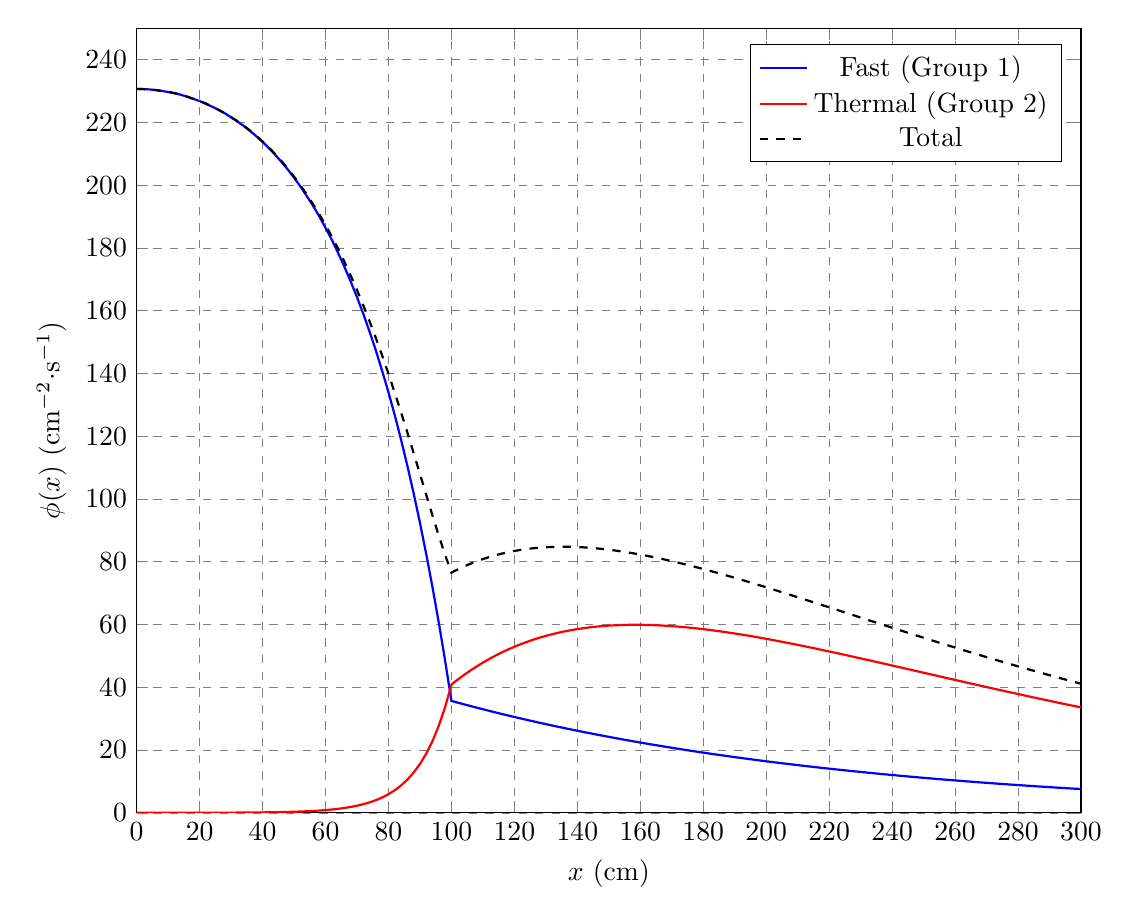
\begin{tikzpicture} \begin{axis}
[scale=1.75,
 xmin=0,    xmax=300,
 ymin=0, ymax=250,
 grid=major, 
 major grid style={color=gray,line width=0.2pt, dashed},
 xlabel=$x$ (cm),
 ylabel=$\phi(x)$ (cm$^{-2}\cdot$s$^{-1}$),
]

\addplot[line width=0.8pt, color=blue] coordinates {
 ( 0.00 , 2.306e+02 ) 
 ( 2.00 , 2.306e+02 ) 
 ( 4.00 , 2.305e+02 ) 
 ( 6.00 , 2.303e+02 ) 
 ( 8.00 , 2.300e+02 ) 
 ( 10.00 , 2.297e+02 ) 
 ( 12.00 , 2.293e+02 ) 
 ( 14.00 , 2.288e+02 ) 
 ( 16.00 , 2.282e+02 ) 
 ( 18.00 , 2.275e+02 ) 
 ( 20.00 , 2.268e+02 ) 
 ( 22.00 , 2.259e+02 ) 
 ( 24.00 , 2.250e+02 ) 
 ( 26.00 , 2.240e+02 ) 
 ( 28.00 , 2.229e+02 ) 
 ( 30.00 , 2.216e+02 ) 
 ( 32.00 , 2.203e+02 ) 
 ( 34.00 , 2.189e+02 ) 
 ( 36.00 , 2.173e+02 ) 
 ( 38.00 , 2.156e+02 ) 
 ( 40.00 , 2.138e+02 ) 
 ( 42.00 , 2.118e+02 ) 
 ( 44.00 , 2.097e+02 ) 
 ( 46.00 , 2.074e+02 ) 
 ( 48.00 , 2.050e+02 ) 
 ( 50.00 , 2.024e+02 ) 
 ( 52.00 , 1.996e+02 ) 
 ( 54.00 , 1.966e+02 ) 
 ( 56.00 , 1.935e+02 ) 
 ( 58.00 , 1.901e+02 ) 
 ( 60.00 , 1.864e+02 ) 
 ( 62.00 , 1.826e+02 ) 
 ( 64.00 , 1.784e+02 ) 
 ( 66.00 , 1.740e+02 ) 
 ( 68.00 , 1.693e+02 ) 
 ( 70.00 , 1.643e+02 ) 
 ( 72.00 , 1.590e+02 ) 
 ( 74.00 , 1.533e+02 ) 
 ( 76.00 , 1.473e+02 ) 
 ( 78.00 , 1.408e+02 ) 
 ( 80.00 , 1.340e+02 ) 
 ( 82.00 , 1.267e+02 ) 
 ( 84.00 , 1.189e+02 ) 
 ( 86.00 , 1.106e+02 ) 
 ( 88.00 , 1.018e+02 ) 
 ( 90.00 , 9.242e+01 ) 
 ( 92.00 , 8.243e+01 ) 
 ( 94.00 , 7.180e+01 ) 
 ( 96.00 , 6.049e+01 ) 
 ( 98.00 , 4.846e+01 ) 
 ( 100.00 , 3.565e+01 ) 
 ( 100.00 , 3.565e+01 ) 
 ( 102.00 , 3.510e+01 ) 
 ( 104.00 , 3.456e+01 ) 
 ( 106.00 , 3.403e+01 ) 
 ( 108.00 , 3.350e+01 ) 
 ( 110.00 , 3.299e+01 ) 
 ( 112.00 , 3.248e+01 ) 
 ( 114.00 , 3.198e+01 ) 
 ( 116.00 , 3.149e+01 ) 
 ( 118.00 , 3.100e+01 ) 
 ( 120.00 , 3.053e+01 ) 
 ( 122.00 , 3.006e+01 ) 
 ( 124.00 , 2.959e+01 ) 
 ( 126.00 , 2.914e+01 ) 
 ( 128.00 , 2.869e+01 ) 
 ( 130.00 , 2.825e+01 ) 
 ( 132.00 , 2.781e+01 ) 
 ( 134.00 , 2.739e+01 ) 
 ( 136.00 , 2.696e+01 ) 
 ( 138.00 , 2.655e+01 ) 
 ( 140.00 , 2.614e+01 ) 
 ( 142.00 , 2.574e+01 ) 
 ( 144.00 , 2.534e+01 ) 
 ( 146.00 , 2.495e+01 ) 
 ( 148.00 , 2.457e+01 ) 
 ( 150.00 , 2.419e+01 ) 
 ( 152.00 , 2.382e+01 ) 
 ( 154.00 , 2.345e+01 ) 
 ( 156.00 , 2.309e+01 ) 
 ( 158.00 , 2.273e+01 ) 
 ( 160.00 , 2.238e+01 ) 
 ( 162.00 , 2.204e+01 ) 
 ( 164.00 , 2.170e+01 ) 
 ( 166.00 , 2.137e+01 ) 
 ( 168.00 , 2.104e+01 ) 
 ( 170.00 , 2.071e+01 ) 
 ( 172.00 , 2.039e+01 ) 
 ( 174.00 , 2.008e+01 ) 
 ( 176.00 , 1.977e+01 ) 
 ( 178.00 , 1.947e+01 ) 
 ( 180.00 , 1.917e+01 ) 
 ( 182.00 , 1.887e+01 ) 
 ( 184.00 , 1.858e+01 ) 
 ( 186.00 , 1.830e+01 ) 
 ( 188.00 , 1.801e+01 ) 
 ( 190.00 , 1.774e+01 ) 
 ( 192.00 , 1.746e+01 ) 
 ( 194.00 , 1.720e+01 ) 
 ( 196.00 , 1.693e+01 ) 
 ( 198.00 , 1.667e+01 ) 
 ( 200.00 , 1.641e+01 ) 
 ( 202.00 , 1.616e+01 ) 
 ( 204.00 , 1.591e+01 ) 
 ( 206.00 , 1.567e+01 ) 
 ( 208.00 , 1.543e+01 ) 
 ( 210.00 , 1.519e+01 ) 
 ( 212.00 , 1.495e+01 ) 
 ( 214.00 , 1.472e+01 ) 
 ( 216.00 , 1.450e+01 ) 
 ( 218.00 , 1.427e+01 ) 
 ( 220.00 , 1.406e+01 ) 
 ( 222.00 , 1.384e+01 ) 
 ( 224.00 , 1.363e+01 ) 
 ( 226.00 , 1.342e+01 ) 
 ( 228.00 , 1.321e+01 ) 
 ( 230.00 , 1.301e+01 ) 
 ( 232.00 , 1.281e+01 ) 
 ( 234.00 , 1.261e+01 ) 
 ( 236.00 , 1.241e+01 ) 
 ( 238.00 , 1.222e+01 ) 
 ( 240.00 , 1.204e+01 ) 
 ( 242.00 , 1.185e+01 ) 
 ( 244.00 , 1.167e+01 ) 
 ( 246.00 , 1.149e+01 ) 
 ( 248.00 , 1.131e+01 ) 
 ( 250.00 , 1.114e+01 ) 
 ( 252.00 , 1.097e+01 ) 
 ( 254.00 , 1.080e+01 ) 
 ( 256.00 , 1.063e+01 ) 
 ( 258.00 , 1.047e+01 ) 
 ( 260.00 , 1.031e+01 ) 
 ( 262.00 , 1.015e+01 ) 
 ( 264.00 , 9.991e+00 ) 
 ( 266.00 , 9.838e+00 ) 
 ( 268.00 , 9.686e+00 ) 
 ( 270.00 , 9.537e+00 ) 
 ( 272.00 , 9.390e+00 ) 
 ( 274.00 , 9.246e+00 ) 
 ( 276.00 , 9.104e+00 ) 
 ( 278.00 , 8.963e+00 ) 
 ( 280.00 , 8.825e+00 ) 
 ( 282.00 , 8.690e+00 ) 
 ( 284.00 , 8.556e+00 ) 
 ( 286.00 , 8.424e+00 ) 
 ( 288.00 , 8.294e+00 ) 
 ( 290.00 , 8.167e+00 ) 
 ( 292.00 , 8.041e+00 ) 
 ( 294.00 , 7.917e+00 ) 
 ( 296.00 , 7.795e+00 ) 
 ( 298.00 , 7.675e+00 ) 
 ( 300.00 , 7.557e+00 ) 
};

\addplot[line width=0.8pt, color=red] coordinates {
 ( 0.00 , 5.163e-03 ) 
 ( 2.00 , 5.260e-03 ) 
 ( 4.00 , 5.554e-03 ) 
 ( 6.00 , 6.057e-03 ) 
 ( 8.00 , 6.787e-03 ) 
 ( 10.00 , 7.771e-03 ) 
 ( 12.00 , 9.047e-03 ) 
 ( 14.00 , 1.066e-02 ) 
 ( 16.00 , 1.268e-02 ) 
 ( 18.00 , 1.517e-02 ) 
 ( 20.00 , 1.823e-02 ) 
 ( 22.00 , 2.197e-02 ) 
 ( 24.00 , 2.654e-02 ) 
 ( 26.00 , 3.211e-02 ) 
 ( 28.00 , 3.888e-02 ) 
 ( 30.00 , 4.710e-02 ) 
 ( 32.00 , 5.710e-02 ) 
 ( 34.00 , 6.923e-02 ) 
 ( 36.00 , 8.397e-02 ) 
 ( 38.00 , 1.019e-01 ) 
 ( 40.00 , 1.236e-01 ) 
 ( 42.00 , 1.499e-01 ) 
 ( 44.00 , 1.819e-01 ) 
 ( 46.00 , 2.207e-01 ) 
 ( 48.00 , 2.677e-01 ) 
 ( 50.00 , 3.248e-01 ) 
 ( 52.00 , 3.941e-01 ) 
 ( 54.00 , 4.782e-01 ) 
 ( 56.00 , 5.802e-01 ) 
 ( 58.00 , 7.040e-01 ) 
 ( 60.00 , 8.542e-01 ) 
 ( 62.00 , 1.036e+00 ) 
 ( 64.00 , 1.258e+00 ) 
 ( 66.00 , 1.526e+00 ) 
 ( 68.00 , 1.852e+00 ) 
 ( 70.00 , 2.247e+00 ) 
 ( 72.00 , 2.726e+00 ) 
 ( 74.00 , 3.307e+00 ) 
 ( 76.00 , 4.013e+00 ) 
 ( 78.00 , 4.869e+00 ) 
 ( 80.00 , 5.908e+00 ) 
 ( 82.00 , 7.169e+00 ) 
 ( 84.00 , 8.698e+00 ) 
 ( 86.00 , 1.055e+01 ) 
 ( 88.00 , 1.281e+01 ) 
 ( 90.00 , 1.554e+01 ) 
 ( 92.00 , 1.885e+01 ) 
 ( 94.00 , 2.288e+01 ) 
 ( 96.00 , 2.776e+01 ) 
 ( 98.00 , 3.368e+01 ) 
 ( 100.00 , 4.086e+01 ) 
 ( 100.00 , 4.086e+01 ) 
 ( 102.00 , 4.243e+01 ) 
 ( 104.00 , 4.392e+01 ) 
 ( 106.00 , 4.531e+01 ) 
 ( 108.00 , 4.662e+01 ) 
 ( 110.00 , 4.785e+01 ) 
 ( 112.00 , 4.900e+01 ) 
 ( 114.00 , 5.008e+01 ) 
 ( 116.00 , 5.109e+01 ) 
 ( 118.00 , 5.203e+01 ) 
 ( 120.00 , 5.290e+01 ) 
 ( 122.00 , 5.372e+01 ) 
 ( 124.00 , 5.446e+01 ) 
 ( 126.00 , 5.515e+01 ) 
 ( 128.00 , 5.579e+01 ) 
 ( 130.00 , 5.637e+01 ) 
 ( 132.00 , 5.690e+01 ) 
 ( 134.00 , 5.738e+01 ) 
 ( 136.00 , 5.781e+01 ) 
 ( 138.00 , 5.819e+01 ) 
 ( 140.00 , 5.853e+01 ) 
 ( 142.00 , 5.883e+01 ) 
 ( 144.00 , 5.909e+01 ) 
 ( 146.00 , 5.931e+01 ) 
 ( 148.00 , 5.949e+01 ) 
 ( 150.00 , 5.964e+01 ) 
 ( 152.00 , 5.975e+01 ) 
 ( 154.00 , 5.983e+01 ) 
 ( 156.00 , 5.988e+01 ) 
 ( 158.00 , 5.990e+01 ) 
 ( 160.00 , 5.990e+01 ) 
 ( 162.00 , 5.986e+01 ) 
 ( 164.00 , 5.980e+01 ) 
 ( 166.00 , 5.971e+01 ) 
 ( 168.00 , 5.960e+01 ) 
 ( 170.00 , 5.947e+01 ) 
 ( 172.00 , 5.932e+01 ) 
 ( 174.00 , 5.914e+01 ) 
 ( 176.00 , 5.895e+01 ) 
 ( 178.00 , 5.874e+01 ) 
 ( 180.00 , 5.851e+01 ) 
 ( 182.00 , 5.826e+01 ) 
 ( 184.00 , 5.800e+01 ) 
 ( 186.00 , 5.772e+01 ) 
 ( 188.00 , 5.743e+01 ) 
 ( 190.00 , 5.713e+01 ) 
 ( 192.00 , 5.681e+01 ) 
 ( 194.00 , 5.648e+01 ) 
 ( 196.00 , 5.614e+01 ) 
 ( 198.00 , 5.579e+01 ) 
 ( 200.00 , 5.543e+01 ) 
 ( 202.00 , 5.506e+01 ) 
 ( 204.00 , 5.468e+01 ) 
 ( 206.00 , 5.430e+01 ) 
 ( 208.00 , 5.390e+01 ) 
 ( 210.00 , 5.350e+01 ) 
 ( 212.00 , 5.309e+01 ) 
 ( 214.00 , 5.268e+01 ) 
 ( 216.00 , 5.226e+01 ) 
 ( 218.00 , 5.183e+01 ) 
 ( 220.00 , 5.140e+01 ) 
 ( 222.00 , 5.097e+01 ) 
 ( 224.00 , 5.053e+01 ) 
 ( 226.00 , 5.009e+01 ) 
 ( 228.00 , 4.965e+01 ) 
 ( 230.00 , 4.920e+01 ) 
 ( 232.00 , 4.875e+01 ) 
 ( 234.00 , 4.830e+01 ) 
 ( 236.00 , 4.784e+01 ) 
 ( 238.00 , 4.738e+01 ) 
 ( 240.00 , 4.693e+01 ) 
 ( 242.00 , 4.647e+01 ) 
 ( 244.00 , 4.601e+01 ) 
 ( 246.00 , 4.555e+01 ) 
 ( 248.00 , 4.509e+01 ) 
 ( 250.00 , 4.463e+01 ) 
 ( 252.00 , 4.417e+01 ) 
 ( 254.00 , 4.371e+01 ) 
 ( 256.00 , 4.325e+01 ) 
 ( 258.00 , 4.279e+01 ) 
 ( 260.00 , 4.233e+01 ) 
 ( 262.00 , 4.188e+01 ) 
 ( 264.00 , 4.142e+01 ) 
 ( 266.00 , 4.097e+01 ) 
 ( 268.00 , 4.051e+01 ) 
 ( 270.00 , 4.006e+01 ) 
 ( 272.00 , 3.961e+01 ) 
 ( 274.00 , 3.917e+01 ) 
 ( 276.00 , 3.872e+01 ) 
 ( 278.00 , 3.828e+01 ) 
 ( 280.00 , 3.784e+01 ) 
 ( 282.00 , 3.740e+01 ) 
 ( 284.00 , 3.696e+01 ) 
 ( 286.00 , 3.653e+01 ) 
 ( 288.00 , 3.610e+01 ) 
 ( 290.00 , 3.567e+01 ) 
 ( 292.00 , 3.524e+01 ) 
 ( 294.00 , 3.482e+01 ) 
 ( 296.00 , 3.440e+01 ) 
 ( 298.00 , 3.399e+01 ) 
 ( 300.00 , 3.357e+01 ) 
};

\addplot[line width=0.8pt, color=black, dashed] coordinates {
 ( 0.00 , 2.306e+02 ) 
 ( 2.00 , 2.306e+02 ) 
 ( 4.00 , 2.305e+02 ) 
 ( 6.00 , 2.303e+02 ) 
 ( 8.00 , 2.300e+02 ) 
 ( 10.00 , 2.297e+02 ) 
 ( 12.00 , 2.293e+02 ) 
 ( 14.00 , 2.288e+02 ) 
 ( 16.00 , 2.282e+02 ) 
 ( 18.00 , 2.275e+02 ) 
 ( 20.00 , 2.268e+02 ) 
 ( 22.00 , 2.260e+02 ) 
 ( 24.00 , 2.250e+02 ) 
 ( 26.00 , 2.240e+02 ) 
 ( 28.00 , 2.229e+02 ) 
 ( 30.00 , 2.217e+02 ) 
 ( 32.00 , 2.204e+02 ) 
 ( 34.00 , 2.189e+02 ) 
 ( 36.00 , 2.174e+02 ) 
 ( 38.00 , 2.157e+02 ) 
 ( 40.00 , 2.139e+02 ) 
 ( 42.00 , 2.120e+02 ) 
 ( 44.00 , 2.099e+02 ) 
 ( 46.00 , 2.077e+02 ) 
 ( 48.00 , 2.053e+02 ) 
 ( 50.00 , 2.027e+02 ) 
 ( 52.00 , 2.000e+02 ) 
 ( 54.00 , 1.971e+02 ) 
 ( 56.00 , 1.940e+02 ) 
 ( 58.00 , 1.908e+02 ) 
 ( 60.00 , 1.873e+02 ) 
 ( 62.00 , 1.836e+02 ) 
 ( 64.00 , 1.797e+02 ) 
 ( 66.00 , 1.756e+02 ) 
 ( 68.00 , 1.712e+02 ) 
 ( 70.00 , 1.666e+02 ) 
 ( 72.00 , 1.617e+02 ) 
 ( 74.00 , 1.566e+02 ) 
 ( 76.00 , 1.513e+02 ) 
 ( 78.00 , 1.457e+02 ) 
 ( 80.00 , 1.399e+02 ) 
 ( 82.00 , 1.338e+02 ) 
 ( 84.00 , 1.276e+02 ) 
 ( 86.00 , 1.212e+02 ) 
 ( 88.00 , 1.146e+02 ) 
 ( 90.00 , 1.080e+02 ) 
 ( 92.00 , 1.013e+02 ) 
 ( 94.00 , 9.468e+01 ) 
 ( 96.00 , 8.825e+01 ) 
 ( 98.00 , 8.214e+01 ) 
 ( 100.00 , 7.651e+01 ) 
 ( 100.00 , 7.651e+01 ) 
 ( 102.00 , 7.753e+01 ) 
 ( 104.00 , 7.847e+01 ) 
 ( 106.00 , 7.934e+01 ) 
 ( 108.00 , 8.012e+01 ) 
 ( 110.00 , 8.084e+01 ) 
 ( 112.00 , 8.148e+01 ) 
 ( 114.00 , 8.206e+01 ) 
 ( 116.00 , 8.258e+01 ) 
 ( 118.00 , 8.303e+01 ) 
 ( 120.00 , 8.343e+01 ) 
 ( 122.00 , 8.377e+01 ) 
 ( 124.00 , 8.406e+01 ) 
 ( 126.00 , 8.429e+01 ) 
 ( 128.00 , 8.448e+01 ) 
 ( 130.00 , 8.462e+01 ) 
 ( 132.00 , 8.471e+01 ) 
 ( 134.00 , 8.476e+01 ) 
 ( 136.00 , 8.477e+01 ) 
 ( 138.00 , 8.474e+01 ) 
 ( 140.00 , 8.467e+01 ) 
 ( 142.00 , 8.457e+01 ) 
 ( 144.00 , 8.443e+01 ) 
 ( 146.00 , 8.426e+01 ) 
 ( 148.00 , 8.406e+01 ) 
 ( 150.00 , 8.383e+01 ) 
 ( 152.00 , 8.357e+01 ) 
 ( 154.00 , 8.328e+01 ) 
 ( 156.00 , 8.297e+01 ) 
 ( 158.00 , 8.264e+01 ) 
 ( 160.00 , 8.228e+01 ) 
 ( 162.00 , 8.190e+01 ) 
 ( 164.00 , 8.150e+01 ) 
 ( 166.00 , 8.108e+01 ) 
 ( 168.00 , 8.064e+01 ) 
 ( 170.00 , 8.018e+01 ) 
 ( 172.00 , 7.971e+01 ) 
 ( 174.00 , 7.922e+01 ) 
 ( 176.00 , 7.872e+01 ) 
 ( 178.00 , 7.820e+01 ) 
 ( 180.00 , 7.767e+01 ) 
 ( 182.00 , 7.713e+01 ) 
 ( 184.00 , 7.658e+01 ) 
 ( 186.00 , 7.602e+01 ) 
 ( 188.00 , 7.545e+01 ) 
 ( 190.00 , 7.487e+01 ) 
 ( 192.00 , 7.428e+01 ) 
 ( 194.00 , 7.368e+01 ) 
 ( 196.00 , 7.307e+01 ) 
 ( 198.00 , 7.246e+01 ) 
 ( 200.00 , 7.185e+01 ) 
 ( 202.00 , 7.122e+01 ) 
 ( 204.00 , 7.060e+01 ) 
 ( 206.00 , 6.996e+01 ) 
 ( 208.00 , 6.933e+01 ) 
 ( 210.00 , 6.869e+01 ) 
 ( 212.00 , 6.805e+01 ) 
 ( 214.00 , 6.740e+01 ) 
 ( 216.00 , 6.676e+01 ) 
 ( 218.00 , 6.611e+01 ) 
 ( 220.00 , 6.546e+01 ) 
 ( 222.00 , 6.481e+01 ) 
 ( 224.00 , 6.416e+01 ) 
 ( 226.00 , 6.351e+01 ) 
 ( 228.00 , 6.286e+01 ) 
 ( 230.00 , 6.220e+01 ) 
 ( 232.00 , 6.155e+01 ) 
 ( 234.00 , 6.090e+01 ) 
 ( 236.00 , 6.026e+01 ) 
 ( 238.00 , 5.961e+01 ) 
 ( 240.00 , 5.896e+01 ) 
 ( 242.00 , 5.832e+01 ) 
 ( 244.00 , 5.768e+01 ) 
 ( 246.00 , 5.704e+01 ) 
 ( 248.00 , 5.640e+01 ) 
 ( 250.00 , 5.577e+01 ) 
 ( 252.00 , 5.513e+01 ) 
 ( 254.00 , 5.451e+01 ) 
 ( 256.00 , 5.388e+01 ) 
 ( 258.00 , 5.326e+01 ) 
 ( 260.00 , 5.264e+01 ) 
 ( 262.00 , 5.202e+01 ) 
 ( 264.00 , 5.141e+01 ) 
 ( 266.00 , 5.080e+01 ) 
 ( 268.00 , 5.020e+01 ) 
 ( 270.00 , 4.960e+01 ) 
 ( 272.00 , 4.900e+01 ) 
 ( 274.00 , 4.841e+01 ) 
 ( 276.00 , 4.782e+01 ) 
 ( 278.00 , 4.724e+01 ) 
 ( 280.00 , 4.666e+01 ) 
 ( 282.00 , 4.609e+01 ) 
 ( 284.00 , 4.552e+01 ) 
 ( 286.00 , 4.495e+01 ) 
 ( 288.00 , 4.439e+01 ) 
 ( 290.00 , 4.384e+01 ) 
 ( 292.00 , 4.329e+01 ) 
 ( 294.00 , 4.274e+01 ) 
 ( 296.00 , 4.220e+01 ) 
 ( 298.00 , 4.166e+01 ) 
 ( 300.00 , 4.113e+01 ) 
};

\legend{Fast (Group 1),Thermal (Group 2),Total}
\end{axis}
\end{tikzpicture}
\caption{Neutron scalar flux distributions in a two-group reflected system.}
 \label{Fig:neutronics_twoGroupReflectedReactor_ScalarFlux}
\end{center}
\end{figure}

\subsection{Two-Group Nuclear Criticality}

In the previous examples we focused on non-multiplying media. Of course, here we are most interested in the question of the criticality condition and finding the effective multiplication factor. In the prior treatment, the one-speed approximation was made, which we know to be overly simplistic for the analysis of nuclear reactors. We can, however, gain insight into the physics of reactors if we study the case of two energy groups. 

For this model we assume that all neutrons are born fast in group 1, they thermalize from group 1 into group 2, but cannot upscatter back into group 1. As before, we eliminate the time derivative term (because the goal is to make the reactor in steady state), discard the internal source (since fission is the dominant mechanism for making neutrons), and then apply a multiplication factor $1/k$ on the fission term to balance the equation. One further simplification is to assume the nuclear properties are not functions of position. (The case of a homogenized reactor.)

The two-group neutron diffusion equations are then
\begin{align}
  &-D_1 \nabla^2 \phi_1(\pos) + \Sigma_{R1} \phi_1(\pos) = \frac{1}{k} \bigg( \nu\Sigma_{f1} \phi_1(\pos) + \nu\Sigma_{f2} \phi_2(\pos) \bigg) , \\*
  &-D_2 \nabla^2 \phi_2(\pos) + \Sigma_{R2} \phi_2(\pos) = \Sigma_{s,1\rightarrow 2} \phi_1(\pos) .
\end{align}
Note that there is two-way coupling between the groups. The source term of the group 2 (thermal) equation is the downscattering from group 1 (fast). Conversely, the source term of the group 1 (fast) equation is fission both from fast and thermal neutrons. To proceed with solving them we can introduce the buckling approximation. First, we assume that the space-energy dependent scalar flux can be factorized into the product of an energy spectrum and a shape function:
\begin{align}
  \phi(\pos,E) = \Phi(E) f(\pos).
\end{align}
If we integrate both sides of this equation over an energy group $g$, we get
\begin{align}
  \int_g \phi(\pos,E) dE &= \int_g  \Phi(E) f(\pos) dE, \nonumber
  \phi_g(\pos) = \Phi_g f(\pos) .
\end{align}
Second, we assume the shape function follows the buckling equation:
\begin{align}
  \nabla^2 f(\pos) + B^2 f(\pos) = 0,
\end{align}
where $B^2$ is the geometric buckling from before. Applying the separability assumption, to the equations we get
\begin{align}
  &-D_1 \Phi_1 \nabla^2  f(\pos) + \Sigma_{R1} \Phi_1 f(\pos) = \frac{1}{k} \bigg( \nu\Sigma_{f1} \Phi_1 f(\pos) + \nu\Sigma_{f2} \Phi_2 f(\pos) \bigg) , \\*
  &-D_2 \Phi_2 \nabla^2  f(\pos) + \Sigma_{R2} \Phi_2 f(\pos) = \Sigma_{s,1\rightarrow 2} \Phi_1 f(\pos) .
\end{align}
Solving the buckling equation for $\nabla^2 f = -B^2 f$ and inserting this into the equations, produces an algebraic system of equations for which there is a common factor of the shape function $f(\pos)$ that we can cancel out. After doing these operations, we have
\begin{align}
  &B^2 D_1 \Phi_1  + \Sigma_{R1} \Phi_1 = \frac{1}{k} \bigg( \nu\Sigma_{f1} \Phi_1  + \nu\Sigma_{f2} \Phi_2 \bigg) , \\*
  &B^2 D_2 \Phi_2  + \Sigma_{R2} \Phi_2  = \Sigma_{s,1\rightarrow 2} \Phi_1  .
\end{align}

Recall from the one-speed case that $B^2 D$ is the effective leakage cross section. By extension, $B^2 D_g$ is the effective leakage section for energy group $g$, where the buckling $B^2$ is a purely geometric effect that is inversely proportional to the size of the system and $D_g$ is the group diffusion coefficient that is proportional to how rapidly neutrons within that energy group migrate down the gradient of the shape function.

Because the multiplication factor only appears in a single equation, we can directly solve for it. (If this is not the case, then we have to set up a system of equations and solve an eigenvalue problem.) To solve this, divide the thermal equation by $\Phi_1$ and solve for the ratio of the thermal-to-fast scalar fluxes:
\begin{align}
  &\frac{\Phi_2}{\Phi_1}  = \frac{ \Sigma_{s,1\rightarrow 2} }{ B^2 D_2  + \Sigma_{R2} }  .
\end{align}
This equation states that the flux ratio is the rate of downscattering from the fast group to the loss rate from thermal neutrons leaking out or being absorbed. 

Next, we divide the fast group equation by $\Phi_1$ and then substitute in the thermal-to-fast scalar flux ratio from that we just obtained from the thermal group equation: 
\begin{align}
  B^2 D_1   + \Sigma_{R1}  
  &= \frac{1}{k} \bigg( \nu\Sigma_{f1}  + \nu\Sigma_{f2} \frac{\Phi_2}{\Phi_1} \bigg) \nonumber \\
  &= \frac{1}{k} \left[ \nu\Sigma_{f1}  + \nu\Sigma_{f2} \left( \frac{ \Sigma_{s,1\rightarrow 2} }{ B^2 D_2  + \Sigma_{R2} } \right) \right] .
\end{align}
Now we can explicitly solve for the multiplication factor $k$:
\begin{align}
  k = \frac{ \nu\Sigma_{f1} }{ B^2 D_1 + \Sigma_{R1} } + \frac{ \nu\Sigma_{f2} }{ B^2 D_2 + \Sigma_{R2} } \frac{ \Sigma_{s,1\rightarrow 2} }{ B^2 D_1  + \Sigma_{R1} }
\end{align}

In principle, we could stop here, but we can look closely and find a physical interpretation of this result and relate it to the six-factor formula. The first term corresponds to the fission from fast neutrons and the second one corresponds to the fission from thermal neutrons. The thermal fission term is more complicated because neutrons need to manage to successfully slow down to thermalize, avoiding leaking out as a fast neutron or being absorbed by the nuclear resonances.

To get to the six-factor formula, we introduce the group diffusion length,
\begin{align}
  L_g^2 = \frac{D_g}{\Sigma_{Rg}} . \nonumber
\end{align}
Solving for the diffusion coefficient $D_g = \Sigma_{Rg} L_g^2$ and factoring out the removal cross sections,
\begin{align}
  k = \frac{ \nu\Sigma_{f1} }{ \Sigma_{R1} } \frac{ 1 }{ 1 + B^2 L_1^2  } + \frac{ \nu\Sigma_{f2} }{ \Sigma_{R2} } \frac{1}{ 1 + B^2 L_2^2 } \frac{ \Sigma_{s,1\rightarrow 2} }{\Sigma_{R1}} \frac{1}{ 1  + B^2 L_1^2 }
\end{align}
Based on the reasoning from Sec.~\ref{Sec:neutronics_oneSpeedEffectiveMultipicationFactor}, we can interpret the $( 1 + B^2 L_g^2 )^{-1}$ terms as the fast and thermal non-leakage probabilities,
\begin{subequations}
\begin{align}
  P_{FNL} &= \frac{ 1 }{ 1 + B^2 L_1^2  } , \\
  P_{TNL} &= \frac{ 1 }{ 1 + B^2 L_2^2  } .
\end{align}
\end{subequations}
Next, we look at the ratio of the downscattering cross section $\Sigma_{s,1 \rightarrow 2}$ to the fast removal cross section $\Sigma_{R2}$. We show this is the resonance escape probability $p$ based on the following chain of reasoning:
\begin{align}
  p = 
  &\ \text{probability that a neutron is not absorbed in a resonance} \nonumber \\
  = &\ \frac{\text{rate fast neutrons downscatter into the thermal group}}{\text{rate fast neutrons downscatter and are absorbed in the resonances}} \nonumber \\
  = &\ \frac{\text{rate fast neutrons downscatter into the thermal group}}{\text{rate fast neutrons are removed from the fast group}} \nonumber \\
  = &\ \frac{\Sigma_{s,1 \rightarrow 2}}{\Sigma_{R1}} .
\end{align}
For the remaining two thermal terms, we need to delineate between the fuel and moderator. Here we denote fuel isotopes with an $F$ superscript and moderator isotopes with an $M$ superscript. The first of these is the thermal fission factor defined by
\begin{align}
  \eta 	&= \ \frac{\text{rate fission neutrons are produced in the fuel}}{\text{rate neutrons are absorbed in the fuel}} \nonumber \\
  		&= \ \frac{\nu\Sigma_f^F}{\Sigma_a^F} .
\end{align}
The second is the thermal utilization factor defined as
\begin{align}
  f 	&= \ \frac{\text{rate neutrons are absorbed the fuel}}{\text{rate neutrons are absorbed in the fuel or moderator}} \nonumber \\
  		&= \ \frac{\Sigma_{a2}^F}{\Sigma_{a2}^F + \Sigma_{a2}^M} \nonumber \\
		&= \ \frac{\Sigma_{a2}^F}{\Sigma_{a2}} .
\end{align}
Since all neutrons are normally only cause fission in the fuel, we can write $\nu\Sigma_f = \nu\Sigma_f^F$. Since the thermal neutrons cannot upscatter, the thermal removal cross section is simply the absorption cross section $\Sigma_{R2} = \Sigma_{a2}$. We can then multiply and divide
\begin{align}
  \frac{ \nu\Sigma_{f2} }{ \Sigma_{R2} } = \frac{ \nu\Sigma_{f2}^F }{ \Sigma_{a2} } \nonumber
\end{align}
by the absorption cross section of the fuel to obtain
\begin{align}
  \frac{ \nu\Sigma_{f2} }{ \Sigma_{R2} } = \frac{ \nu\Sigma_{f2}^F }{ \Sigma_{a2}^F } \frac{ \Sigma_{a2}^F }{ \Sigma_{a2} } = \eta f .
\end{align}
Inserting these definitions into the expression for the effective multiplication factor we get
\begin{align}
  k = \frac{ \nu\Sigma_{f1} }{ \Sigma_{R1} } P_{FNL} + \eta f p P_{TNL} P_{FNL} .
\end{align}

The second term looks suspiciously close to the six-factor formula, except that it is missing the fast fission factor. This quantity is defined as
\begin{align}
  \epsilon = \ \frac{\text{rate fission neutrons are produced from fast and thermal neutrons}}{\text{rate fission neutrons are produced from just thermal neutrons}}. \nonumber
\end{align}
To simplest way to get at the fast fission factor is to define the contribution to fission neutron production from fast neutrons as $k_1$ and the contribution from thermal neutrons as $k_2$. Recall that these correspond to the first and second terms in the expression for the effective multiplication factor. We can then write
\begin{align}
  k = k_1 + k_2 = \frac{ k_1 + k_2 }{ k_2 } k_2  = \left( 1 + \frac{k_1}{k_2} \right) k_2 = \epsilon k_2 .
\end{align}
This implies, after a bit of algebraic manipulation that the fast fission factor is
\begin{align}
  \epsilon = 1 + \frac{ \nu\Sigma_{f1} }{ \nu\Sigma_{f2} } \frac{ \Sigma_{R2} }{ \Sigma_{s,1\rightarrow 2}} ( 1 + B^2 L_2^2 ) .
\end{align}
Given all of these terms, we then get the six-factor formula:
\begin{align}
  k = \eta f p \epsilon P_{FNL} P_{TNL} .
\end{align}

The definition of the fast-fission factor is admittedly a bit unwieldy and not particularly intuitive. It is worth noting that these definitions are not the only groupings that could be reasonably made, but are perhaps the ones most commonly seen in textbooks. Despite these shortcomings, we were able to show a connection between the expression for the effective multiplication factor and the physical quantities describing the neutron lifecycle from the six-factor formula.

\subsection{Modified One-Group Diffusion Theory and Migration Area}

An approximation that can be made in large thermal reactors is that the leakage effects from thermal neutrons are negligible. This is justified because the mean-free path of thermal neutrons is significantly smaller than that of fast neutrons and very small relative to the size of the overall geometry. This motivates the following approximation:
\begin{align}
  -D_2 \nabla^2 \phi_2 = B^2 D_2 \phi_2 \approx 0.
\end{align}
Based on this, the thermal group flux can be solved explicitly for the in terms of the fast flux from the thermal neutron diffusion equation:
\begin{align}
  \phi_2(\pos) = \frac{\Sigma_{s,1\rightarrow 2}}{\Sigma_{a2}} \phi_1(\pos) .
\end{align}
Here we assumed as before that the material properties are uniformly homogenized throughout the reactor.

From here, we return to the fast neutron diffusion equation and insert the above relation for the thermal flux:
\begin{align}
  -D_1 \nabla^2 \phi_1(\pos) + \Sigma_{R1} \phi_1(\pos) 
  &= \nu\Sigma_{f1} \phi_1(\pos) + \nu\Sigma_{f2} \phi_2(\pos) \nonumber \\
  &= \left( \nu\Sigma_{f1} + \nu\Sigma_{f2} \frac{\Sigma_{s,1\rightarrow 2}}{\Sigma_{a2}} \right) \phi_1(\pos) .
\end{align}
Now we divide by $-D_1$ and write the diffusion coefficient in terms of the diffusion length and removal cross section using $D_1 = \Sigma_{R1} L_1^2$ to get
\begin{align}
  &\nabla^2\phi_1(\pos) + \left[ \frac{ \nu\Sigma_{f1} + \nu\Sigma_{f2} ( \Sigma_{s,1\rightarrow 2} / \Sigma_{a2} ) - \Sigma_{R1} }{ \Sigma_{R1} L_1^2 } \right] \phi_1(\pos), \nonumber \\
  &\nabla^2\phi_1(\pos) + \left[ \frac{ k_\infty - 1 }{ L_1^2 } \right] \phi_1(\pos).
\end{align}
Here we define the effective multiplication factor for an infinite medium as
\begin{align}
  k_\infty = \frac{  \nu\Sigma_{f1} }{ \Sigma_{R1} } + \frac{ \nu\Sigma_{f2} }{ \Sigma_{R1} } \frac{\Sigma_{s,1\rightarrow 2}}{\Sigma_{a2}} .
\end{align}

However, we are not quite done yet and can improve this further, albeit by using a bit of a hack. It turns out using $L_1^2$ (with the fast diffusion length) alone in the denominator is not quite as accurate at representing the migration of neutrons as we would like. So it would be nice then to put back in some effect for the thermal neutrons migrating. We can do this in rather ad hoc manner by replacing the $L_1^2$ with a quantity called the \emph{migration area}, which is the sum of the squares of the diffusion lengths for fast and thermal neutrons:
\begin{align}
  M^2 = L_1^2 + L_2^2 .
\end{align}
(In the next chapter we will discuss a different approach for estimating the fast diffusion length.) Making this substitution we get
\begin{align}
  &\nabla^2\phi_1(\pos) + \left[ \frac{ k_\infty - 1 }{ M^2 } \right] \phi_1(\pos).
\end{align}

This form looks mathematically identical to the buckling equation and all the solution techniques we used before for one-speed problems can be applied here. Going through the exact same analysis, we find that the effective multiplication factor predicted by this model is
\begin{align}
  k = \frac{ k_\infty }{ 1 + B^2 M^2 } .
\end{align}
This result should not be surprising as it is just $k_\infty$ times the non-leakage probability, except here we used the migration area and a more complicated estimate of the infinite multiplication factor.

This modified one-group diffusion theory is sometimes referred to as the one-and-a-half group diffusion theory in that it solves a one-group problem for the fast neutrons, but embeds information from the thermal neutrons in an approximate manner. Returning to where we began this discussion to close it out, the accuracy of this modified one-group diffusion theory depends on the the migration of thermal neutrons being very small relative to the size of the reactor. This is a reasonable approximation in a typically large light-water reactor that is hundreds of thermal neutron mean-free paths wide, but becomes questionable as the size of the reactor gets smaller.

\subsection{Group Constant Collapse}

As mentioned at the beginning this section, a reactor analysis often involves performing multiple calculations. These are typically done on smaller portions of the reactor with finer energy group structures or larger portions using coarser group structures. A key application of the fine-group calculations is to use the group fluxes to determine group constants for the coarse energy discretizations. This is an entire topic onto itself, so here we do a simple example and use the previous two-group calculations to determine one-group cross sections. 

The one-group absorption cross section is
\begin{align}
  \Sigma_a 
  &= \dfrac{ \displaystyle\int_{E_2}^{E_0} \Sigma_a(E) \Phi(E) dE }{ \displaystyle\int_{E_2}^{E_0} \Phi(E) dE } \nonumber \\
  &= \dfrac{ \displaystyle\int_{E_2}^{E_1} \Sigma_a(E) \Phi(E) dE + \int_{E_1}^{E_0} \Sigma_a(E) \Phi(E) dE }{ \displaystyle\int_{E_2}^{E_1} \Phi(E) dE + \int_{E_1}^{E_0} \Phi(E) dE } \nonumber \\
  &= \dfrac{ \left[ \dfrac{ \displaystyle\int_{E_2}^{E_1} \Sigma_a(E) \Phi(E) dE }{ \displaystyle\int_{E_2}^{E_1} \Phi(E) dE } \right] \phi_1 
  			+ \left[ \dfrac{ \displaystyle\int_{E_1}^{E_0} \Sigma_a(E) \Phi(E) dE  }{ \displaystyle\int_{E_1}^{E_0} \Phi(E) dE } \right] \phi_2  }{ \phi_2 + \phi_1 } \nonumber \\
  &= \frac{ \Sigma_{a2} \phi_2 + \Sigma_{a1} \phi_1 }{ \phi_2 + \phi_1 } \nonumber \\
  &= \frac{ \Sigma_{R1} \phi_1 - \Sigma_{s,1\rightarrow 2} \phi_1 + \Sigma_{a2} \phi_2 }{ \phi_1 + \phi_2 } .
\end{align}
We assume here that there is no upscatter as before so that the thermal removal cross section is just the thermal absorption cross section. Returning to our buckled thermal neutron equation,
\begin{align}
  B^2 D_2 \phi_2 + \Sigma_{a2} \phi_2 = \Sigma_{s,1\rightarrow 2} \phi_1 , \nonumber
\end{align}
we can algebraically relate $\phi_2$ to $\phi_1$ and substitute in the expression for the collapsed one-speed absorption cross section:
\begin{align}
  \Sigma_a = \frac{ ( \Sigma_{R1} - \Sigma_{s,1\rightarrow 2} ) ( B^2 D_2 + \Sigma_{a2} ) + \Sigma_{s,1\rightarrow 2} \Sigma_{a2} }{ B^2 D_2 + \Sigma_{a2} + \Sigma_{s,1\rightarrow 2} } .
\end{align}
Note that the fast scalar flux divided out. The collapsed one-group cross section depends on both the material properties, as well as the geometry and leakage effects by way of the buckling coefficient. 

This process can be repeated for the other group constants as well. Note that the collapse for diffusion coefficient is a bit ambiguous given that it is unlike the other terms in how it was derived. Often, they are treated just like the other cross sections, but this may not be the best way to compute them. We can also generalize this notion to an arbitrary group collapse, but we are not going to cover that in these notes. However, next, we will provide the matrix formulations needed to go down that path.

\subsection{Multigroup Criticality Equations in Matrix Form}

While the two-group model is nice for both pedagogical examples and some reactor analyses at the full-core scale, there are a wide range of problems for which more energy groups are necessary. As stated earlier, for a problem involving $G$ energy groups we end up with $G$ coupled equations. The most efficient way to represent these is using a matrix formulation.

To begin, we first restate the multigroup diffusion equation for group $g$:
\begin{align}
  &\frac{1}{v_g} \dho{\phi_g}{t} - \nabla \cdot D_g(\pos) \nabla \phi_g(\pos,t) + \Sigma_{Rg}(\pos) \phi_g(\pos,t) \nonumber \\*
  &= \sum_{\substack{g' =1 \\ g' \ne g}}^G  \Sigma_{s,g' \rightarrow g}(\pos,t) \phi_{g'}(\pos,t) + \chi_g \sum_{g'=1}^G   \nu\Sigma_{fg'}(\pos,t) \phi_{g'}(\pos,t) + Q_{g}(\pos) . \nonumber
\end{align}
Now we introduce the column vector for the scalar fluxes that we are trying to determine:
\begin{align}
  \boldsymbol\phi = \left[ \begin{array}{c} \phi_1 \\ \phi_2 \\ \vdots \\ \phi_G \end{array} \right] .
\end{align}
The internal source vector $\mathbf{q}$ is defined similarly.

We will first write down the time-dependent version with a fixed source and then pose the criticality problem. Starting with the time-derivative term, we have the inverse speeds for each group as a diagonal matrix:
\begin{align}
  \mathbf{V}^{-1} = \left[ \begin{array}{c c c c c}
  v_1^{-1} 	& 0			& \cdots	& 0				& 0			\\
  0			& v_2^{-1}	& \cdots	& 0				& 0			\\
  \vdots	& \vdots	& \ddots	& \vdots		& \vdots	\\
  0			& 0			& \cdots	& v_{G-1}^{-1}	& 0			\\
  0			& 0			& \cdots	& 0				& v_G^{-1}	\\ \end{array} \right] .
\end{align}
The diffusion operator is likewise a diagonal matrix
\begin{align}
  \mathbf{D} = \left[ \begin{array}{c c c c c}
  \nabla \cdot D_1(\pos) \nabla 	& 0								& \cdots	& 0				& 0			\\
  0									& \nabla \cdot D_2(\pos) \nabla & \cdots	& 0				& 0			\\
  \vdots							& \vdots						& \ddots	& \vdots		& \vdots	\\
  0									& 0								& \cdots	& \nabla \cdot D_{G-1}(\pos) \nabla 	& 0			\\
  0									& 0								& \cdots	& 0				& \nabla \cdot D_G(\pos) \nabla 	\\ \end{array} \right] .
\end{align}
The removal cross section is likewise a diagonal matrix
\begin{align}
  \boldsymbol\Sigma_R = \left[ \begin{array}{c c c c c}
  \Sigma_{R1}(\pos) 	& 0			& \cdots	& 0				& 0			\\
  0			& \Sigma_{R2}(\pos)	& \cdots	& 0				& 0			\\
  \vdots	& \vdots	& \ddots	& \vdots		& \vdots	\\
  0			& 0			& \cdots	& \Sigma_{R,G-1}(\pos)	& 0			\\
  0			& 0			& \cdots	& 0				& \Sigma_{RG}(\pos)	\\ \end{array} \right] .
\end{align}
The scattering matrix is a full matrix with the diagonal element of zero (because it is subtracted from the right-hand side and moved to the left):
\begin{align}
  \boldsymbol\Sigma_s = \left[ \begin{array}{c c c c c}
  0	& \Sigma_{s,2\rightarrow 1}(\pos)			& \cdots	& \Sigma_{s,G-1\rightarrow 1}(\pos)				& \Sigma_{s,G\rightarrow 1}(\pos)			\\
  \Sigma_{s,1\rightarrow 2}(\pos)			& 0	& \cdots	& \Sigma_{s,G-1\rightarrow 2}(\pos)				& \Sigma_{s,G\rightarrow 2}(\pos)				\\
  \vdots	& \vdots	& \ddots	& \vdots		& \vdots	\\
  \Sigma_{s,1\rightarrow G-1}(\pos)		& \Sigma_{s,2\rightarrow G-1}(\pos)		& \cdots	& 0	& \Sigma_{s,G\rightarrow G-1}(\pos)				\\
  \Sigma_{s,1\rightarrow G}(\pos)		& \Sigma_{s,1\rightarrow G}(\pos)		& \cdots	& \Sigma_{s,G-1\rightarrow G}(\pos)		& 0	\\ \end{array} \right] .
\end{align}
If there is a single thermal group, then the scattering matrix is lower triangular. The fission term is lumped into a full-matrix
\begin{align}
  \mathbf{F} &= 
  \left[ \begin{array}{c} \chi_1 \\ \chi_2 \\ \vdots \\ \chi_G \end{array} \right]
  \left[ \begin{array}{c c c c} \nu\Sigma_{f1} & \nu\Sigma_{f2} & \cdots & \nu\Sigma_{f,G} \end{array} \right] \nonumber \\
  &= \left[ \begin{array}{c c c c c}
  \chi_1 \nu\Sigma_{f1}	& \chi_1 \nu\Sigma_{f2}			& \cdots	& \chi_1 \nu\Sigma_{f,G-1}				& \chi_1 \nu\Sigma_{fG}			\\
  \chi_2 \nu\Sigma_{f1}	& \chi_2 \nu\Sigma_{f2}			& \cdots	& \chi_2 \nu\Sigma_{f,G-1}				& \chi_2 \nu\Sigma_{fG}			\\
  \vdots	& \vdots	& \ddots	& \vdots		& \vdots	\\
  \chi_{G-1} \nu\Sigma_{f1}	& \chi_{G-1} \nu\Sigma_{f2}			& \cdots	& \chi_{G-1} \nu\Sigma_{f,G-1}	& \chi_{G-1} \nu\Sigma_{fG}			\\
  \chi_G \nu\Sigma_{f1}	& \chi_G \nu\Sigma_{f2}			& \cdots	& \chi_G \nu\Sigma_{f,G-1}				& \chi_G \nu\Sigma_{fG}			\\	 \end{array} \right] .
\end{align}

Given these definitions, we can write the time-dependent multigroup diffusion equation in matrix-vector form
\begin{align}
  \left( \mathbf{V}^{-1} \dho{}{t} - \mathbf{D} + \boldsymbol\Sigma_R \right) \boldsymbol\phi
  =  \boldsymbol\Sigma_s \boldsymbol\phi + \mathbf{F} \boldsymbol\phi + \mathbf{q} .
\end{align}

The criticality neutron diffusion problem is ``derived'' using the same approach as before. The time-derivative term is eliminated, the internal source vector is set to zero, and a factor of $1/k$ is applied to the fission term. We also move the scattering term to the left-hand side. This criticality problem is then
\begin{align}
  \left( - \mathbf{D} + \boldsymbol\Sigma_R - \boldsymbol\Sigma_s \right) \boldsymbol\phi
  =  \frac{1}{k} \mathbf{F} \boldsymbol\phi  .
\end{align}
For reasons we will discuss next, this is called the $k$-eigenvalue neutron diffusion equation. 

\subsection{Interpretation of the $k$-Eigenvalue Equation}

As a shorthand, we define the net loss matrix as the left-hand side of the equation,
\begin{align}
  \mathbf{M} = - \mathbf{D} + \boldsymbol\Sigma_R - \boldsymbol\Sigma_s .
\end{align}
We also define the fission matrix acting on the scalar flux vector as as the fission source vector
\begin{align}
  \mathbf{f} = \mathbf{F} \boldsymbol\phi .
\end{align}
The equation is then written in shorthand form as
\begin{align}
  \mathbf{M} \boldsymbol\phi = \frac{1}{k} \mathbf{f} .
\end{align}
Now we apply the inverse of the net loss operator on both sides of the equation to isolate the flux and multiply by $k$,
\begin{align}
  k \boldsymbol\phi =  \mathbf{M}^{-1} \mathbf{f} .
\end{align}
Next, apply the fission operator to both sides
\begin{align}
   \mathbf{F} \mathbf{M}^{-1} \mathbf{f} = k \mathbf{f}.
\end{align}
By inspecting this result, we note $\mathbf{F} \mathbf{M}^{-1}$ as matrix acting on the fission source $\mathbf{f}$, which equals a constant $k$ times the fission source $\mathbf{f}$. This means that $k$ can be interpreted as the \emph{eigenvalue of the fission source}.

A question that remains is what $\mathbf{F} \mathbf{M}^{-1}$ means physically. The net loss matrix $\mathbf{M}$ describes the physics of diffusion (neutrons migrating along the negative gradient), removal from the group, and gains into the group from inscattering. Note that this specifically \emph{excludes} fission. Taking the inverse of $\mathbf{M}$ and applying it onto a source vector, in this case the fission source vector, takes neutrons from that source and propagates them based on the physics that is included. In other words, the neutrons migrate until they either leak out or are absorbed. Because fission is specifically excluded, this means the history of those neutrons, at least according to the application of the matrix $\mathbf{M}^{-1}$ end. The result of $\mathbf{M}^{-1} \mathbf{f}$ is the resulting scalar flux for diffusing neutrons from the fission source through a single fission generation.

Now when we apply the fission matrix $\mathbf{F}$ onto this scalar flux from $\mathbf{M}^{-1} \mathbf{f}$, we get the resulting fission source. The eigenvalue equation tells us that this is equal to the fission source $\mathbf{f}$, but scaled by some constant factor $k$, and hence the name, the effective multiplication factor. This leads to the common interpretation for the effective multiplication factor:
\begin{align}
  k = \ \frac{\text{number of fission neutrons in generation $i$}}{\text{number of fission neutrons in generation $i-1$}} .
\end{align}
Basically, each fission generation, the eigenvalue equation enhances the fission source by a multiplier $k$. The special case of criticality is therefore when the system is in perfect balance such that (on average) the number of neutrons in the fission sources between subsequent generations is constant.

Before leaving this topic, we note that applying the factor of $1/k$ onto the fission source term is not particularly physical for cases that are off-critical. A natural question is whether the equation in means anything physically. The short answer is that strictly speaking, no it does not. The $k$-eigenvalue form of the neutron diffusion (or transport) equation is only representative of physical reality in the particular case where a system is at criticality. Otherwise, it is a mathematical representation of a fictitious system where the fission source has been artificially adjusted to preserve balance.

Now just because it is not necessarily physical does not mean it is not useful. Solving an eigenvalue problem is much easier than solving a time-dependent one---that does mean it is easy, just easier. If the system is off critical, the eigenvalue tells us whether it is subcritical or supercritical and gives us a measure of how much. While interpreting what this means in terms of the physical design parameters is tricky, it does allow us to do engineering design work.

Regarding the advantage versus time-dependent problems, there is another type of eigenvalue problem that appears in the context of nuclear kinetics. If we assume that the space and energy variables are separable from time (note that this is not guaranteed for general problems, but holds up extremely well so long as a system has multiplying material and is not too subcritical), we can conclude that the behavior follows an exponential as $e^{\alpha t}$. Going through the analysis (neglecting the effect of delayed neutrons here), we arrive at the following equation:
\begin{align}
  \left( \alpha \mathbf{V}^{-1}  - \mathbf{D} + \boldsymbol\Sigma_R \right) \boldsymbol\phi
  =  \boldsymbol\Sigma_s \boldsymbol\phi + \mathbf{F} \boldsymbol\phi .
\end{align}
We can show that this is also an eigenvalue problem where $\alpha$ is the eigenvalue. The difference here is an $\alpha/v$ term. For $\alpha > 0$, the system is evidently supercritical. The $\alpha/v$ term applies an absorption term that preferentially removes slower neutrons. Physically, this means that for an exponentially growing population, the transient is driven by the faster neutrons with the slower ones lagging behind and not making much difference. This ``hardens'' the neutron spectrum in that there are fewer slower neutrons. Conversely, for $\alpha < 0$, this can be interpreted as a source that is inversely proportional to the neutron speed. Physically, this means that the rate that an exponentially decreasing population is limited by the slower neutrons, which are enhanced in the neutron spectrum.

Returning to the question of the $k$-eigenvalue problem versus a time-dependent one, we see that the time-dependent one has a shift in the neutron spectrum depending on whether the system is supercritical or subcritical. The $k$-eigenvalue globally adjusts the fission source, which has a much smaller impact on the spectrum. Therefore the $k$-eigenvalue equation does not yield the correct energy spectrum for a non-critical system. 

While this may seem undesirable, there is a practical sense that this is actually beneficial. Because the neutron spectrum is quite stable in the $k$-eigenvalue problem versus a time-dependent or $\alpha$-eigenvalue problem, we can more easily execute a criticality search. If the neutron spectrum changes significantly between design iterations, it makes determining the next guess difficult. So this is one key advantage of the $k$-eigenvalue problem and one of the many reasons it is used in the design of nuclear reactors.

%%%%%%%%%%%%%%%%%%%%%%%%%%%%%%%%%%%%%%%%%%%%%%%%%%%%%%%%%%%%%%%%%%%%%%%%%%%%%%%%
\section{Numerical Solution Techniques}

Based on the the examples that we did, it may be clear that the algebra required to obtain analytical solutions quickly becomes very complicated to the point of being unworkable, especially once we begin using multiple regions and multiple energy groups. This motivates exploring numerical methods that can be used to obtain approximate solutions of the neutron transport and diffusion equations. All of these methods require some form of spatial and energy (and direction for transport) discretization of some type. Note that the material presented in this section barely scratches the surface of this topic---indeed numerous careers have been and are devoted to the broad field of studying, developing, and implementing a wide array of numerical schemes.

The material in this section will focus on 1-D planar or slab geometry. First, we will discuss the discrete ordinates method, which is one of the many ways to solve the neutron transport equation. This will be done in the context of a steady-state, fixed-source problem with a single energy group. Next, we explore an analogous approach to solving the neutron diffusion equation for the same scenario. Then, we extend both (with the focus on diffusion, but the strategy is much the same for transport) to include multiple energy groups and then to the tackle $k$-eigenvalue problem.

\subsection{Neutron Transport 1-D Discrete Ordinates Method}

To begin this, we write the steady-state, 1-D neutron transport equation in slab geometry as
\begin{align}
  \mu \dho{}{x} \psi(x,\mu) + \Sigma_t(x) \psi(x,\mu) = q(x,\mu) ,
\end{align}
where, for compactness, we lumped scattering, fission, and internal sources into the right-hand side source $q(x,\mu)$. We have two independent variables, the spatial coordinate $x$ and the direction cosine $\mu$ with respect to the $x$-axis. Both of these need to be discretized in some manner.

\subsubsection{Spatial Discretization}

\begin{figure}[tb!]
\begin{center}
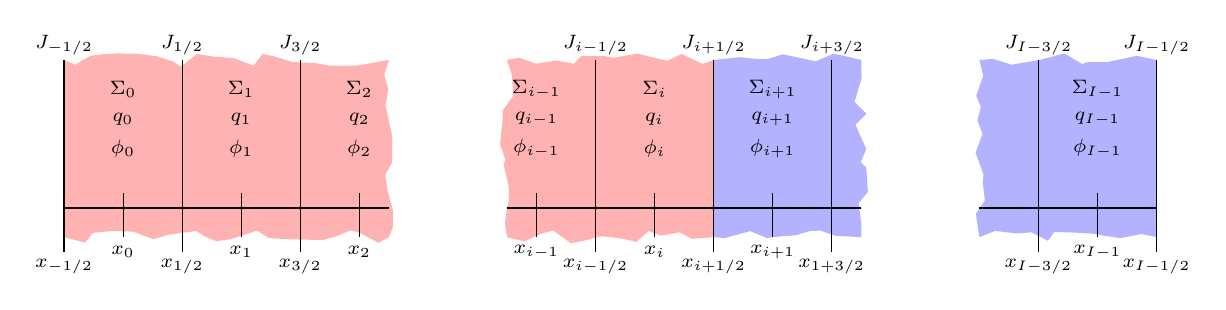
\begin{tikzpicture}[scale=0.75] \scriptsize
% left side boundary section
\fill[red!30, decoration={random steps,segment length=0.2cm}] (0,-0.5) decorate{-- (5.5,-0.5)} decorate{-- (5.5,2.5)} decorate{-- (0,2.5)} -- cycle;
\draw[thick] (0,0) -- (5.5,0);
\draw (0,-0.75) -- (0,2.5);
\draw (1,-0.5)  -- (1,0.25);
\draw (2,-0.75) -- (2,2.5);
\draw (3,-0.5)  -- (3,0.25);
\draw (4,-0.75) -- (4,2.5);
\draw (5,-0.5)  -- (5,0.25);
\node at (0,-1) 	{$x_{-1/2}$};
\node at (1,-0.75) 	{$x_0$};
\node at (2,-1) 	{$x_{1/2}$};
\node at (3,-0.75) 	{$x_1$};
\node at (4,-1) 	{$x_{3/2}$};
\node at (5,-0.75) 	{$x_2$};
\node at (0,2.75) {$J_{-1/2}$}; \node at (2,2.75) {$J_{1/2}$}; \node at (4,2.75) {$J_{3/2}$};
\node at (1,2)   {$\Sigma_0$}; \node at (1,1.5)   {$q_0$}; 	\node at (1,1)   {$\phi_0$};
\node at (3,2)   {$\Sigma_1$}; \node at (3,1.5)   {$q_1$}; 	\node at (3,1)   {$\phi_1$};
\node at (5,2)   {$\Sigma_2$}; \node at (5,1.5)   {$q_2$}; 	\node at (5,1)   {$\phi_2$};

% interior section
\fill[red!30,  decoration={random steps,segment length=0.2cm}] (7.5,-0.5) decorate{-- (11,-0.5)} -- (11,2.5) decorate{-- (7.5,2.5)} decorate{-- cycle};
\fill[blue!30, decoration={random steps,segment length=0.2cm}] (11,-0.5)  decorate{-- (13.5,-0.5)} decorate{-- (13.5,2.5)} decorate{-- (11,2.5)} -- cycle;
\draw[thick] (7.5,0) -- (13.5,0);
\draw (8, -0.5)   -- (8, 0.25);
\draw (9, -0.75)  -- (9, 2.5);
\draw (10,-0.5)   -- (10,0.25);
\draw (11,-0.75)  -- (11,2.5);
\draw (12,-0.5)   -- (12,0.25);
\draw (13,-0.75)  -- (13,2.5);
%\draw (14,-0.5)   -- (14,0.25);
\node at (8,-0.75) 	{$x_{i-1}$};
\node at (9,-1) 	{$x_{i-1/2}$};
\node at (10,-0.75) {$x_{i}$};
\node at (11,-1) 	{$x_{i+1/2}$};
\node at (12,-0.75) {$x_{i+1}$};
\node at (13,-1) 	{$x_{1+3/2}$};
%\node at (14,-0.75) {$x_{i+2}$};
\node at (9,2.75) {$J_{i-1/2}$}; \node at (11,2.75) {$J_{i+1/2}$}; \node at (13,2.75) {$J_{i+3/2}$};
\node at (8, 2)   {$\Sigma_{i-1}$}; 	\node at (8, 1.5) {$q_{i-1}$}; 	\node at (8, 1)   {$\phi_{i-1}$};
\node at (10,2)   {$\Sigma_{i}$}; 		\node at (10,1.5) {$q_{i}$}; 	\node at (10,1)   {$\phi_{i}$};
\node at (12,2)   {$\Sigma_{i+1}$}; 	\node at (12,1.5) {$q_{i+1}$}; 	\node at (12,1)   {$\phi_{i+1}$};
%\node at (14,2)   {$\Sigma_{i+2}$}; 	\node at (14,1.5) {$q_{i+2}$}; 	\node at (14,1)   {$\phi_{i+2}$};

% interior section
\fill[blue!30,  decoration={random steps,segment length=0.2cm}] (15.5,-0.5) decorate{-- (18.5,-0.5)} -- (18.5,2.5) decorate{-- (15.5,2.5)} decorate{-- cycle};
\draw[thick] (15.5,0) -- (18.5,0);
\draw (18.5, -0.75)   -- (18.5, 2.5);
\draw (17.5, -0.5)  -- (17.5, 0.25);
\draw (16.5, -0.75)  -- (16.5, 2.5);
\node at (16.5,-1) 	{$x_{I-3/2}$};
\node at (17.5,-0.75) {$x_{I-1}$};
\node at (18.5,-1) 	{$x_{I-1/2}$};
\node at (16.5,2.75) {$J_{I-3/2}$}; \node at (18.5,2.75) {$J_{I-1/2}$};
\node at (17.5, 2)   {$\Sigma_{I-1}$}; 	\node at (17.5, 1.5) {$q_{I-1}$}; 	\node at (17.5, 1)   {$\phi_{I-1}$};

\end{tikzpicture}
\caption{Grid or stencil for the cell-centered finite differencing scheme for the numerical solutions of neutron transport and diffusion.}
\label{Fig:neutronics_finiteDifferenceStencil}
\end{center}
\end{figure}

First, we introduce \emph{cell-centered} spatial discretization, which is depicted in Fig.~\ref{Fig:neutronics_finiteDifferenceStencil}. The rationale of this choice is it allows us to strictly enforce particle balance within each zone where outgoing currents $J$ are given on the edges and reaction rates, by way of the scalar flux $\phi$, are defined at the center. The concept of particle balance states simply that the rate particles are produced from the source plus the rate particles enter must be balanced by the rate particles are absorbed plus the rate they leave. 

This sounds rather obvious and we had not had to worry about it because the differential equations (either neutron transport or diffusion) naturally support particle balance by virtue of how they were derived. The problem is that the process of mapping these differential equations onto a spatial discretization, which converts a calculus problem into algebra one, may or may not preserve the balance of particles depending on how this is done. The cost of enforcing particle balance (or analogously conservation of mass, momentum, and energy if we were solving a thermal fluids problem) has a cost, and that is a more complicated numerical scheme.

The cell-centered spatial discretization breaks the problem into $I$ spatial regions indexed from $i = 0, 1, \ldots, I-1$ (indexing from zero follows the convention from the C programming language that most modern languages use) each having a width $\Delta_i = x_{i+1} - x_i$. The point $x_i$ is the center of the $i$th spatial zone. This implies that $x_{-1/2} = 0$ is the left edge of the slab and $x_{I-1/2} = a$ is the right edge. Material properties (e.g., cross sections) and sources are taken to be within each spatial zone. Ideally, we choose the spatial discretization to line up with the geometric regions of the problem. If we cannot do this, or do not wish to for some reason, then we need to find some average value of the material properties.

\subsubsection{Angular Discretization}

We also need to discretize the direction or angular variable $\mu$. As the name of the discrete ordinates method implies, we pick a set of discrete directions $\mu_n$ that the neutrons travel along. We have a large amount of flexibility to pick the angular discretization, but in 1-D planar geometry there is one choice that is usually superior to anything else, which is picking the $\mu_n$ to be along the Gauss-Legendre quadrature integration points. Why this is is because the right-hand side $q(x,\mu)$ includes the scattering and fission sources that contain integrals over the angular fluxes. It is therefore beneficial to pick a set of directions that maximize the accuracy of numerically calculating these integrals with the fewest number of points.

For those readers not familiar, with the Gauss-Legendre quadrature set, we do a quick summary. In general, we can write a quadrature rule for numerical integration from the domain of $[-1,1]$ as
\begin{align}
  \int_{-1}^1 f(\mu) d\mu \approx \sum_{n=1}^N w_n f(\mu_n) .
\end{align}
We have quite a bit of freedom to choose the points or abscissa $\mu_n$ and the associated weights $w_n$. One common constraint is to choose the weights such that it correctly integrates the special case of $f(\mu_n) = 1$, a constant. This requires that the sum of the weights add to two:
\begin{align}
  \sum_{n=1}^N w_n = 2.
\end{align}

There exists a special set of $N$ points and weights capable of \emph{exactly} integrating polynomials up an order $2N - 1$, which makes for a very attractive choice. These special points $\mu_n$ are the roots of the $N$th-order Legendre polynomial $P_N(\mu)$ for $n = 0,\ldots,N-1$. The weights can be computed from
\begin{align}
  w_n = \frac{ 2 }{ ( 1 - \mu_n^2 ) \left[ P_N'(\mu_n) \right]^2 } .
\end{align}
So if we use just four of these special points and weights, we can (almost miraculously) integrate up to a seventh-order polynomial exactly. (One might say integrating polynomials is easy, and they would not be wrong; however, the formulas for the integrals can get quite cumbersome and it is usually the case that just using these points and weights is much quicker from both an implementation and an execution standpoint.) 

In practice, the points $\mu_n$ and weights $w_n$ are pre-calculated and put into lookup tables. One nice property is that the points are always symmetric across the zero, so if $\mu_n$ is a point, then so is $-\mu_n$. Furthermore, the weights for both of these are identical. Because of this, we often only need to store half of the information and can just reuse the information for the other half. We often times colloquially refer to these as the $S_N$ Gauss-Legendre set. The case for $N = 16$ is given to high precision in Table~\ref{Table:neutronics_S16GaussLegendreQuadratureWeightsAbscissa}, which is adequate for many applications. 

Note that we usually choose $N$ to be even. The odd-ordered Gauss-Legendre quadrature set includes $\mu_{n-1} = 0$, which creates a potential ``divide by zero'' scenario that would need to be handled as a special case. To avoid having to check for and address this scenario, the simple and agreed-upon solution is just to demand even-ordered quadrature sets.

\begin{table}[tb!]
\caption{$S_{16}$ Gauss-Legendre Quadrature Weights and Abscissa}
\begin{center}
\begin{tabular}{|c|c|c|} \hline
$n$	& $w_n$					& $\mu_n$				\\ \hline
0	& 0.1894506104550685	& 0.0950125098376374	\\
1	& 0.1826034150449236	& 0.2816035507792589	\\
2	& 0.1691565193950025	& 0.4580167776572274	\\
3	& 0.1495959888165767	& 0.6178762444026438	\\
4	& 0.1246289712555339	& 0.7554044083550030	\\
5	& 0.0951585116824928	& 0.8656312023878318	\\
6	& 0.0622535239386479	& 0.9445750230732326	\\
7	& 0.0271524594117541	& 0.9894009349916499	\\ \hline
\end{tabular}
\end{center}
\label{Table:neutronics_S16GaussLegendreQuadratureWeightsAbscissa}
\end{table}%

\subsubsection{Discrete Ordinates Transport Equation}

To proceed we now write the one-speed transport equation for neutrons moving along a single direction $\mu_n$. This is
\begin{align}
  \mu_n \dho{}{x} \psi(x,\mu_n) + \Sigma_t(x) \psi(x,\mu_n) = q(x,\mu_n) . \label{Eq:neutronics_discreteOrdinates_oneSpeedSingleOrdinateTransportEquation}
\end{align}
The right-hand source $q$ contains contributions from scattering, fission, and internal sources:
\begin{align}
  q(x,\mu_n) = \sum_{\ell=0}^L \left( \frac{2\ell+1}{2} \right) P_\ell(\mu_n) \sigma_{s\ell}(x) \phi_\ell(x) + \nu\Sigma_f(x) \phi(x) + Q(x,\mu_n) . \label{Eq:neutronics_discreteOrdinates_oneSpeedRightHandSideSource}
\end{align}
Here $\phi_\ell(x)$ is the $\ell$th Legendre moment of the angular flux, which is approximated by
\begin{subequations}
\begin{align}
  \phi_\ell(x) = \int_{-1}^1 P_\ell(\mu) \psi(x,\mu) d\mu \approx \sum_{n=0}^{N-1} w_n P_\ell(\mu_n) \psi(x,\mu_n) ,
\end{align}
and $\phi(x)$ without the subscript is the standard scalar flux,
\begin{align}
  \phi(x) = \phi_0(x) = \int_{-1}^1 \psi(x,\mu) d\mu \approx \sum_{n=0}^{N-1} w_n \psi(x,\mu_n) .
\end{align}
\end{subequations}
Note that we truncated the sum over Legendre moments in Eq.~\eqref{Eq:neutronics_discreteOrdinates_oneSpeedRightHandSideSource} to order $L$. This is obviously necessary otherwise we would be stuck with having to compute an infinite number of Legendre moments, which would literally take forever. Usually the choice of truncation $L$ is dictated by the expansion order of the nuclear data cross section set. The higher the order, the higher the accuracy, but there is the inherent tradeoff between accuracy and cost in terms of computational time and memory storage requirements.

We then integrate the transport equation in Eq.~\eqref{Eq:neutronics_discreteOrdinates_oneSpeedSingleOrdinateTransportEquation} over a spatial zone or cell. Assuming constant material properties within each cell, we obtain
\begin{align}
  &\int_{x_{i-1/2}}^{x_{i+1/2}} \mu_n \dho{}{x} \psi(x,\mu_n) + \Sigma_t(x_i) \psi(x,\mu_n) dx = \int_{x_{i-1/2}}^{x_{i+1/2}}  q(x,\mu_n) dx, \nonumber \\
 &\mu_n \left[ \psi(x_{i+1/2},\mu_n) - \psi(x_{i-1/2},\mu_n) \right] + \Sigma_{t,i}  \int_{x_{i-1/2}}^{x_{i+1/2}} \psi(x,\mu_n) dx = \int_{x_{i-1/2}}^{x_{i+1/2}}  q(x,\mu_n) dx. \nonumber
\end{align}
Here we let $\Sigma_t(x_i) = \Sigma_{t,i}$. To handle the integrals, we define the cell-averaged quantities
\begin{subequations}
\begin{align}
  \psi_{i,n} 	&= \frac{1}{\Delta_i} \int_{x_{i-1/2}}^{x_{i+1/2}} \psi(x,\mu_n) dx , \\
  q_{i,n} 		&= \frac{1}{\Delta_i} \int_{x_{i-1/2}}^{x_{i+1/2}} q(x,\mu_n) dx .
\end{align}
Substituting in the definition of $q$ into the spatial integral, we see we need to also define the cell-averaged angular flux moments as
\begin{align}
  \phi_{\ell,i,n} 	&= \frac{1}{\Delta_i} \int_{x_{i-1/2}}^{x_{i+1/2}} \phi_\ell(x,\mu_n) dx .
\end{align}
We then note that the first term is the net flow rate for particles moving along a direction $\mu_n$. We define
\begin{align}
  J_{i+1/2,n} &= \mu_n \psi_{i+1/2,n} = \mu_n \psi(x_{i+1/2},\mu_n), \\
  J_{i-1/2,n} &= \mu_n \psi_{i-1/2,n} = \mu_n \psi(x_{i-1/2},\mu_n).
\end{align}
\end{subequations}
Given these definitions, we can then write our balance relationship for particles traveling along direction $\mu_n$ as
\begin{align}
  J_{i+1/2,n} - J_{i-1/2,n} + \Sigma_{t,i} \Delta_i \psi_{i,n} = q_{i,n} \Delta_i . \label{Eq:neutronics_discreteOrdinatesBalanceForm}
\end{align}

Before proceeding to the solution algorithm, we note that $q$ depends on the angular flux $\psi(x,\mu)$ at all $\mu_n$. One might think that one needs to store all values of $\psi(x,\mu_n)$ at all spatial grid points. It turns out this is needlessly wasteful (and impractical in 3-D calculations), and we often can get away with just keeping a running sum of the Legendre moments $\phi_\ell$ at each location for elements we are not currently computing.

\subsubsection{Transport Sweep Algorithm}

The next task is to devise a numerical scheme for solving these equations. One option is to write down the equations for each pair of spatial cell $i$ and ordinate $n$, form a linear system and matrix, and solve the problem. In practice, this would be $I \times N$ equations. While this would not be too large a system to tackle in 1-D, it becomes prohibitive in higher dimensions and with energy dependence, so we opt for a different, matrix-free method called a \emph{transport sweep}. The idea is that we order the equations in a way that we only need to solve for and store the necessary information to solve one equation at a time, discarding all variables that we will not need for subsequent equations.

The one complication here is that the source term $q$ depends on the unknown angular fluxes $\psi_{i,n}$ by way of the flux moments $\phi_{\ell,i}$. The typical way this is addressed is to use a technique called \emph{source iteration} where we guess the flux moments $\phi_{\ell,i}$, compute the sources $q_{i,n}$, solve for angular fluxes $\psi_{i,n}$ and update the flux moments. Assuming the system is subcritical, then this algorithm converges to a solution. (We will address the case of an eigenvalue problem for neutron diffusion. The idea is much the same for transport.)

To proceed with the transport sweep, we write Eq.~\eqref{Eq:neutronics_discreteOrdinatesBalanceForm} in terms of the edge-angular fluxes as
\begin{align}
  \mu_n \left[ \psi_{i+1/2,n} - \psi_{i-1/2,n} \right] + \Sigma_{t,i} \Delta_i \psi_{i,n} = q_{i,n} \Delta_i . \label{Eq:neutronics_discreteOrdinatesTransportEquation}
\end{align}
For now, we assume $q_{i,n}$ is known, and defer discussion of source iteration for a bit. The problem we have is that we have one equation for each cell, but unknowns for both the cell and the edges. First, we can handle the left and right edges via a prescribed boundary conditions:
\begin{subequations}
\begin{align}
  \psi_{-1/2,n}  &= \psi_{-1/2,n},  \quad \mu_n > 0, \\
  \psi_{I-1/2,n} &= \psi_{I-1/2,n}, \quad \mu_n < 0.  
\end{align}
\end{subequations}
This still leaves the interior edges. For this, we simply have to make an ad hoc assumption or closure that describes how the cell-average and edge angular fluxes are related. There are several ways one could handle this, but the the simplest is the \emph{diamond difference relationship} that says the cell-averaged angular flux is the average of the edge angular fluxes,
\begin{align}
  \psi_{i,n} = \frac{1}{2} \left( \psi_{i-1/2,n} + \psi_{i+1/2,n} \right) . \label{Eq:neutronics_diamondDifferenceRelationship}
\end{align}
The diamond difference relationship has good theoretical convergence properties, but also some important drawbacks. Namely, if spatial cells are too optically thick, then the algorithm can lead to non-physical \emph{negative} angular fluxes. In higher dimensions, it becomes difficult to avoid this occurrence and we often employ more sophisticated schemes. While it is good to be aware of this, we are going to proceed anyway as a matter of expedience.

Now we have a sufficient number of equations to solve the problem. Since for $\mu_n > 0$, we are given the information at the left boundary $\psi_{-1/2,n}^b$, we know the information on the left and can solve the equations moving from left to right in a cell-by-cell manner. Using the discrete-ordinates transport equation in Eq.~\eqref{Eq:neutronics_discreteOrdinatesTransportEquation} and the diamond difference relationship in Eq.~\eqref{Eq:neutronics_diamondDifferenceRelationship}, we arrive at the following two equations for each cell with $\mu_n > 0$:
\begin{subequations}
\begin{align}
  \psi_{i,n} &= \left( 1 + \frac{\Sigma_{t,i} \Delta_i}{ 2 | \mu_n | } \right)^{-1} \left( \psi_{i-1/2,n} + \frac{ \Delta_i q_{i,n} }{ 2 | \mu_n | } \right) , \\
  \psi_{i+1/2,n} &= 2 \psi_{i,n} - \psi_{i-1/2,n} .
\end{align}
\end{subequations}

We can then repeat this process for $\mu_n < 0$. Since we are given the right-boundary angular flux $\psi_{I-1/2,n}^b$, we solve the equations going from right to left. We obtain
\begin{subequations}
\begin{align}
  \psi_{i,n} &= \left( 1 + \frac{\Sigma_{t,i} \Delta_i}{ 2 | \mu_n | } \right)^{-1} \left( \psi_{i+1/2,n} + \frac{ \Delta_i q_{i,n} }{ 2 | \mu_n | } \right) , \\
  \psi_{i-1/2,n} &= 2 \psi_{i,n} - \psi_{i+1/2,n} .
\end{align}
\end{subequations}
Note that these results are functionally identical with the roles left- and right-edge angular fluxes swapped.

From here we can solve for all of the given angular fluxes, provided we know the right-hand side source $q_{i,n}$. As we said, in reality we do not know them because they depend on the flux moments that depend on the angular fluxes we are solving for. We address this next by bringing in source iteration.

\subsubsection{Source Iteration}

The first step is we rewrite the discrete ordinates transport equation giving the angular fluxes a superscript iteration index $m$, 
\begin{align}
  \mu_n \left[ \psi_{i+1/2,n}^{(m+1)} - \psi_{i-1/2,n}^{(m+1)} \right] + \Sigma_{t,i} \Delta_i \psi_{i,n}^{(m+1)} = q_{i,n}^{(m)} \Delta_i , \label{Eq:neutronics_discreteOrdinatesTransportEquation_Iteration}
\end{align}
where the source is given in terms of the flux moments as
\begin{align}
  q_{i,n}^{(m)} = \sum_{\ell=0}^L \left( \frac{2\ell+1}{2} \right) P_\ell(\mu_n) \sigma_{s\ell,i} \phi_{\ell,i}^{(m)} + \nu\Sigma_f(x) \phi_i^{(m)} + Q_{i,n}.
\end{align}
where the flux moments are given by
\begin{align}
  \phi_{\ell,i}^{(m)} = \sum_{n=0}^{N-1} w_n \psi_{i,n}^{(m)} 
\end{align}
with the scalar flux $\phi_i = \phi_{0,i}$.

To proceed, we make an initial guess of $\phi_{\ell,i}^{(0)}$ and compute the right-hand side source based upon that. In the absence of better information, setting them equal to zero is as good a choice as any. We then perform transport sweep to obtain $\psi_{i,n}^{(1)}$ and use these angular fluxes to obtain the flux moments $\phi_{\ell,i}^{(1)}$. We then recompute the source, perform another transport sweep, compute updated flux moments, and repeat the process. We continue this until we achieve convergence in whatever order of flux moments are needed for the output results. Often we are most interested in reaction rates, so we only need to converge the scalar fluxes. In general, however, we could converge all of them.

To measure convergence, we often use the scaled Euclidian or L$^2$ norm over all the flux moments in the problem. We compute this each iteration and stop when
\begin{align}
  \dfrac{ \left[ \displaystyle\sum_{\ell=0}^L \sum_{i=0}^{I-1} \left( \phi_{\ell,i}^{(m+1)} - \phi_{\ell,i}^{(m)} \right)^2 \right]^{1/2} }{ \left[ \displaystyle\sum_{\ell=0}^L \sum_{i=0}^{I-1} \left( \phi_{\ell,i}^{(m)} \right)^2 \right]^{1/2} },
\end{align}
where $\epsilon$ is some user-prescribed convergence tolerance for the desired level of accuracy.

Note again during transport sweeps we do not need to actually store the angular fluxes for other cells. Rather, we can accrue the updated flux moments for each spatial cell during the left and right sweeps, discarding the angular fluxes as they are no longer needed.

\subsubsection{Reflecting Boundary Conditions}

In reactor analysis problems, we often solve problems with reflecting boundaries on one or often both faces to take advantage of geometric symmetry. On the left and right sides we have as the boundary conditions
\begin{subequations}
\begin{align}
  \psi_{-1/2,n}  &= \psi_{-1/2,N-n}, \quad \mu_n > 0, \\
  \psi_{I-1/2,n} &= \psi_{I-1/2,N-n}, \quad \mu_n < 0.
\end{align}
\end{subequations}
This implies that the inward angular flux for direction $\mu_n$ is equal to the outward angular flux $\mu_{N-n}$, so we need to know one to find the other.

For the case where only one of the boundaries is reflecting, we have enough information if we perform the sweep starting with the known edge first, computing the new boundary condition, and then performing the sweep in the other direction. 

The case where \emph{both} sides are reflecting is a bit trickier. This is actually quite common as we tend to perform transport calculations on unit fuel pin cells or assemblies. To manage this, we need to iterate on the angular fluxes. This usually involves with guessing a constant in $\mu_n$ angular flux on one of the edges, performing the sweep to the other boundary, computing the boundary fluxes at that other boundary, and then doing the sweep in the backward direction. This results in updated boundary angular fluxes. We then check to see how well the previous guess matches the updated values, typically with the L$^2$ norm meeting some tolerance. If it is not met, we repeat the process using the updated boundary angular fluxes until it does. Note that this is an additional iteration that occurs \emph{within} the standard source iteration.

\subsection{Neutron Diffusion}

We now explore numerical solutions of the neutron diffusion equation in 1-D planar geometry. Contrasting with transport, we only have a single spatial coordinate to discretize as opposed to both space and direction. Another difference is the neutron diffusion equation is a second-order differential equation, whereas the neutron transport equation is first-order. Taken together, this implies a different solution method.

As with transport we use a \emph{cell-centered} spatial discretization, which allows us to enforce particle balance within each zone. Again, particle balance states that the numerical scheme preserves the fact that in each spatial region, the rate particles are produced from the source plus the rate particles enter are balanced by the rate particles are absorbed plus the rate they leave. This is especially important for calculations related to nuclear criticality where we specifically need to know about the balance of neutrons. 

We break the problem into $N$ spatial regions or cells indexed from $i = 0, 1, \ldots, N-1$ each having a width $\Delta_i$. The point $x_i$ is the center of the $i$th spatial zone with $x_{i-1/2}$ and $x_{i+1/2}$ on the left and right respectively. Each spatial zone has its own constant material property, which are here the absorption cross section $\Sigma_{a}(x_i) = \Sigma_{a,i}$, diffusion coefficient $D(x_i) = D_i$, and internal source $q(x_i) = q_i$. We solve for the scalar fluxes $\phi_i$ at the mesh centers. The net currents are defined at the cell edges $J_{i \pm 1/2}$ and are used to describe the flow rates into and out of the zone. 

\subsubsection{Discretion of the Neutron Continuity Equation}

To begin, we start with the neutron continuity equation
\begin{align}
  \frac{dJ}{dx} + \Sigma_a(x) \phi(x) = q(x) .
\end{align}
Here the source $q(x)$ potentially includes fission and internal sources. (For multigroup this includes inscatter into the group where the absorption cross section becomes the removal cross section.) For now we assume that the source is given. We then integrate over a spatial region:
\begin{align}
  &\int_{x_{i-1/2}}^{x_{i+1/2}} \frac{dJ}{dx} + \Sigma_a(x) \phi(x) dx = \int_{x_{i-1/2}}^{x_{i+1/2}} q(x) dx, \nonumber \\
  &J_{i+1/2} - J_{i-1/2} + \int_{x_{i-1/2}}^{x_{i+1/2}} \Sigma_a(x) \phi(x) dx = \int_{x_{i-1/2}}^{x_{i+1/2}} q(x) dx .
\end{align}

Since the absorption cross section is assumed to be spatially constant over the region and equal to $\Sigma_{a,i}$, we can pull it out of the integral. Next, we define the cell-average scalar flux and source to be at the center of the cell,
\begin{subequations}
\begin{align}
  \phi_i 	&= \frac{1}{\Delta_i} \int_{x_{i-1/2}}^{x_{i+1/2}} \phi(x) dx , \\
  q_i 		&= \frac{1}{\Delta_i} \int_{x_{i-1/2}}^{x_{i+1/2}} q(x) dx .
\end{align}
\end{subequations}
Inserting these cell-averaged fluxes and sources we get
\begin{align}
  J_{i+1/2} - J_{i-1/2} + \Sigma_{a,i} \Delta_i \phi_i = q_i \Delta_i .
\end{align}
The next task is to figure out the net currents at the cell-edges. 

\subsubsection{Interface Conditions for Internal Regions}

We handle the currents differently if the cell is an internal region versus a boundary region. First we explore the internal regions, which require us to use the interface condition that the net current must be continuous. Beginning on the left-hand side of a cell centered at $x_i$, we use Fick's law considering that cell and the one immediately to the left (centered about $x_{i-1}$. Fick's law involves the spatial derivative of the scalar flux, which we approximate using a simple differencing scheme. Doing this gives us two equations for the current at $x_{i-1/2}$ that are related to the cell-averaged scalar fluxes on each side of the edge. These equations are
\begin{subequations}
\begin{align}
  J_{i-1/2} &= -D_{i}   \frac{ \phi_{i}     - \phi_{i-i/2} }{ \Delta_{i}/2 }, \label{Eq:neutronics_neutronDiffusionFiniteDifference_FicksLawLeftInterface1} \\
  J_{i-1/2} &= -D_{i-1} \frac{ \phi_{i-1/2} - \phi_{i-1}   }{ \Delta_{i-1}/2 },
\end{align}
\end{subequations}
for the element centered about $x_i$ and $x_{i-1}$ respectively. Note the factor of one-half on the width of the cell is because we take the finite difference to approximate the derivative from the center to the edge, which is half the width.

Both of these equations involve the scalar flux at the cell edge $\phi(x_{i-1/2}) = \phi_{i-1/2}$, which is not part of the discretized neutron continuity equation. However, since we have two equations in terms of the cell-edge scalar flux and the current at that edge, we can eliminate this extra variable by equating the two equations and solving for $\phi_{i-1/2}$. After a bit of algebra, we get
\begin{align}
  \phi_{i-1/2} = \left[ \frac{ D_{i-1} / \Delta_{i-1} }{ D_{i-1}/\Delta_{i-1} + D_{i}/\Delta_{i} } \right] \phi_{i-1} + \left[ \frac{ D_i / \Delta_i }{ D_{i-1}/\Delta_{i-1} + D_{i}/\Delta_{i} } \right] \phi_i . 
\end{align}
If we inspect the terms of brackets, we can see see that if we were to add them together, we would get one. Therefore, we define the term on the left as $\omega_{i-1}$ and have $\omega_i = 1 - \omega_{i-1}$. This allows us to write this more compactly as
\begin{align}
  \phi_{i-1/2} = \omega_{i-1} \phi_{i-1} + ( 1 - \omega_{i-1} ) \phi_i .
\end{align}
Inserting this into Eq.~\eqref{Eq:neutronics_neutronDiffusionFiniteDifference_FicksLawLeftInterface1}, we can then solve for the net current at the left interface:
\begin{align}
  J_{i-1/2} &= -\frac{2 D_{i}}{\Delta_i} \left[ \phi_i - \omega_{i-1} \phi_{i-1} - ( 1 - \omega_{i-1} ) \phi_i \right] \nonumber \\
  			&= -\frac{2 D_{i} \omega_{i-1} }{\Delta_i} ( \phi_i - \phi_{i-1} ) \nonumber \\
			&= -2 \frac{ ( D_{i-1} / \Delta_{i-1} ) ( D_i / \Delta_i ) }{ D_{i-1} / \Delta_{i-1} + D_i / \Delta_i } ( \phi_i - \phi_{i-1} ) \nonumber \\
			&= -\widetilde{D}_{i-1/2} ( \phi_i - \phi_{i-1} ) .
\end{align}

Here we defined as shorthand the edge-averaged diffusion coefficient
\begin{align}
  \widetilde{D}_{i-1/2} = 2 \frac{ ( D_{i-1} / \Delta_{i-1} ) ( D_i / \Delta_i ) }{ D_{i-1} / \Delta_{i-1} + D_i / \Delta_i } . \label{Eq:neutronics_neutronDiffusionFiniteDifference_EdgeAverageDiffusionCoefficient}
\end{align}
At first glance, this may not look like much of an average, but if we set the cell widths to be equal, we can show that this is the harmonic mean of the diffusion coefficients. Note that this is different than what is typically used for the diffusion coefficients in standard finite difference methods where the they are taken in an ad hoc manner to be the arithmetic mean.

We can repeat the process for the current on the right edge $J_{1+1/2}$ by consider the cell at $x_i$ and the one to the right centered about $x_{i+1}$. Applying Fick's law on both sides of the edge gives
\begin{subequations}
\begin{align}
  J_{i+1/2} &= -D_{i}   \frac{ \phi_{i+1/2} - \phi_{i} 		}{ \Delta_{i}/2 	}, \label{Eq:neutronics_neutronDiffusionFiniteDifference_FicksLawRightInterface1} \\
  J_{i+1/2} &= -D_{i+1} \frac{ \phi_{i} 	- \phi_{i-1/2}  }{ \Delta_{i+1}/2 	}.
\end{align}
\end{subequations}
Setting these equal and solving for the cell-edge scalar flux gives
\begin{align}
  \phi_{i+1/2} &=  \left[ \frac{ D_i / \Delta_i }{ D_{i+1}/\Delta_{i+1} + D_{i}/\Delta_{i} } \right] \phi_i + \left[ \frac{ D_{i+1} / \Delta_{i+1} }{ D_{i+1}/\Delta_{i+1} + D_{i}/\Delta_{i} } \right] \phi_{i+1} \nonumber \\
  &= \omega_i \phi_i + ( 1 - \omega_i ) \phi_{i+1},
\end{align}
again noting the terms in brackets sum to one. Inserting this into Eq.~\eqref{Eq:neutronics_neutronDiffusionFiniteDifference_FicksLawRightInterface1} to eliminate the cell-edge scalar flux, we get
\begin{align}
  J_{i+1/2} &= -\frac{2 D_{i}}{\Delta_i} \left[ \omega_i \phi_i + ( 1 - \omega_i ) \phi_{i+1} - \phi_{i}  \right] \nonumber \\
  			&= -\frac{2 D_{i} ( 1- \omega_{i-1} ) }{\Delta_i} ( \phi_{i+1} - \phi_i ) \nonumber \\
			&= -2 \frac{ ( D_{i} / \Delta_{i} ) ( D_{i+1} / \Delta_{i+1} ) }{ D_{i} / \Delta_{i} + D_{i+1} / \Delta_{i+1} } ( \phi_{i+1} - \phi_{i} ) \nonumber \\
			&= -\widetilde{D}_{i+1/2} ( \phi_{i+1} - \phi_{i} ) .
\end{align}
Here again, the edge-averaged diffusion coefficient
\begin{align}
  \widetilde{D}_{i+1/2} = 2 \frac{ ( D_{i} / \Delta_{i} ) ( D_{i+1} / \Delta_{i+1} ) }{ D_{i} / \Delta_{i} + D_{i+1} / \Delta_{i+1} } .
\end{align}
Note that this coefficient is identical to the one in Eq.~\eqref{Eq:neutronics_neutronDiffusionFiniteDifference_EdgeAverageDiffusionCoefficient} by letting $i \rightarrow i+1$, which is comforting.

Plugging these edge net currents back into the discretized neutron continuity equation, we have
\begin{align}
  -\widetilde{D}_{i+1/2} ( \phi_{i+1} - \phi_{i} ) + \widetilde{D}_{i-1/2} ( \phi_i - \phi_{i-1} )  + \Sigma_{a,i} \Delta_i \phi_i = q_i \Delta_i .
\end{align}
Grouping terms we get
\begin{align}
 -\widetilde{D}_{i-1/2} \phi_{i-1} + \left( \widetilde{D}_{i-1/2} + \widetilde{D}_{i+1/2}  + \Sigma_{a,i} \Delta_i \right) \phi_i - \widetilde{D}_{i+1/2} \phi_{i+1}  = q_i \Delta_i .
\end{align}

If we inspect this expression for the cell centered at $x_i$, we notice that its average scalar flux $\phi_i$ is coupled only to the average scalar fluxes to its immediate neighbors. If we write out the equations for each of the interior mesh cells, $i=1, \ldots, N-2$, (we address the boundary cells next) we notice that this forms a tridiagonal system of equations. We can therefore write the coefficients as the subdiagonal (lower) element $\ell_i$, diagonal element $d_i$, the superdiagonal (upper) element $u_i$, and the right-hand side vector element $r_i$ as
\begin{subequations}
\begin{align}
  \ell_i	&= -\widetilde{D}_{i-1/2}, \\
  d_i		&=  \widetilde{D}_{i-1/2} + \widetilde{D}_{i+1/2}  + \Sigma_{a,i} \Delta_i, \\
  u_i		&= -\widetilde{D}_{i+1/2}, \\
  r_i		&=  q_i \Delta_i.
\end{align} 
\end{subequations}
These interior cell equations may then be written generically as
\begin{align}
  \ell_i \phi_{i-1} + d_i \phi_i + u_i \phi_{i+1} = r_i .
\end{align}
It turns out that we get pretty much the exact same results on the boundaries as well. One difference is that on the left and right sides at $i = 0$ and $i = N-1$ we have
\begin{subequations}
\begin{align}
  \ell_0  = 0, \\
  u_{N-1} = 0,
\end{align}
\end{subequations}
which would be outside the bounds of the matrix. We also can get an additional term on the right-hand side vector should there be an inward partial current. Of course, we still need to actually compute the edge diffusion coefficients, which is the next topic.


\subsubsection{Specified Partial Current at a Boundary}

We will look at two cases. The first is where the inward partial current is specified. Following that, we will discuss the albedo boundary conditions, which generalizes to the vacuum and reflecting boundary conditions.

On the left side of the problem, the neutron continuity equation is
\begin{align}
  J_{1/2} - J_{-1/2} + \Sigma_{a,0} \Delta_0 \phi_0 = q_0 \Delta_0 .
\end{align}
From our previous analysis,
\begin{align}
  J_{1/2} = -\widetilde{D}_{1/2} \phi_2 .
\end{align}
The edge-averaged diffusion coefficient can be calculated from Eq.~\eqref{Eq:neutronics_neutronDiffusionFiniteDifference_EdgeAverageDiffusionCoefficient}. We cannot, however, do the same for the net current at the left edge of the problem, $J_{-1/2}$, because the previous analysis only applied to interior elements.

Suppose we are given the incident particle current on the left $J^+$. The Marshak boundary condition on the left where the index $i = 0$ can be written as
\begin{align}
  4 J^+ = \phi_{-1/2} + 2 J_{-1/2} .
\end{align}
As with interior elements, we can use Fick's law with the finite difference approximation of the derivative to relate the boundary net current $J_{-1/2}$ to the scalar flux at the boundary,
\begin{align}
  J_{-1/2} = -D_0 \frac{ \phi_0 - \phi_{-1/2} }{ \Delta_0 / 2 } .
\end{align}
Solving this for $\phi_{-1/2}$ we get
\begin{align}
  \frac{ 2 D_0 }{ \Delta_0 } \phi_{-1/2} = J_{-1/2} + \frac{ 2 D_0 }{ \Delta_0 } \phi_0 .
\end{align}
Here we left on the factor because it will simplify things going forward.

Next, we multiply $2 D_0 / \Delta_0$ onto both sides of the Marshak boundary condition and then insert the result we just obtained,
\begin{align}
  &\frac{ 2 D_0 }{ \Delta_0 } \phi_{-1/2} + \frac{ 2 D_0 }{ \Delta_0 } \cdot 2 J_{-1/2}  = \frac{ 2 D_0 }{ \Delta_0 } \cdot 4 J^+ , \nonumber \\
  &J_{-1/2} + \frac{ 2 D_0 }{ \Delta_0 } \phi_0 + \frac{ 2 D_0 }{ \Delta_0 } \cdot 2 J_{-1/2}  = \frac{ 2 D_0 }{ \Delta_0 } \cdot 4 J^+ .
\end{align}
After a little bit of algebra, we arrive at a form for the net current at the left boundary,
\begin{align}
  J_{-1/2} = -\frac{ 2 D_0 / \Delta_0 }{ 1 + 2 ( 2 D_0 / \Delta_0 ) } \phi_0 + \frac{ 2 D_0 / \Delta_0 }{ 1 + 2 ( 2 D_0 / \Delta_0 ) } 4 J^+ . \nonumber
\end{align}
We can then rewrite this as
\begin{align}
  J_{-1/2} 
  &= -2 \frac{ ( 1/4 )  ( D_0 / \Delta_0 ) }{ 1/4 + D_0 / \Delta_0 } \phi_0 + 2 \frac{ ( 1/4 ) ( D_0 / \Delta_0 )  }{ 1/4 + D_0 / \Delta_0 }  4 J^+  \nonumber \\*
  &= -\widetilde{D}_{-1/2} \phi_0 + 4 \widetilde{D}_{-1/2} J^+ ,
\end{align}
where the left-boundary diffusion coefficient is
\begin{align}
  \widetilde{D}_{-1/2} = 2 \frac{ ( 1/4 ) ( D_0 / \Delta_0 )  }{ 1/4 + D_0 / \Delta_0 } . \label{Eq:neutronics_finiteDifference_EdgeDiffusionCoefficient_LeftVacuum}
\end{align}
Writing it in this form may seem a bit strange and cumbersome, however, in the next section we consider the albedo boundary condition and are able to easily relate this to the forthcoming result.

First, however, we will quickly go through the same process for the right boundary centered at $x_{N-1}$ where the inward partial current $J^-$ is specified. The neutron continuity equation is
\begin{align}
  J_{N-1/2} - J_{N-3/2} + \Sigma_{a,N-1} \Delta_{N-1} \phi_{N-1} = q_{N-1} \Delta_{N-1} .
\end{align}
Here we already handled $J_{N-3/2} = -D_{N-3/2} \phi_{N-2}$ since it is an interior element. For the other particle current we write the Marshak boundary condition on the right boundary:
\begin{align}
  4 J^- = \phi_{N-1/2} - 2 J_{N-1/2} .
\end{align}
Using Fick's law with the finite difference approximation of the derivative, we get the net current at the boundary is
\begin{align}
  J_{N-1/2} = -D_{N-1} \frac{ \phi_{N-1/2} - \phi_{N-1} }{ \Delta_{N-1} / 2 } .
\end{align}
Solving this for the edge scalar flux gives
\begin{align}
   \frac{ 2 D_{N-1} }{ \Delta_{N-1} } \phi_{N-1/2} = -J_{N-1/2} + \frac{ 2 D_{N-1} }{ \Delta_{N-1} } \phi_{N-1} .
\end{align}
As before, we multiply the Marshak boundary condition by $2 D_{N-1}/\Delta_{N-1}$ as before and insert this result. After going through very similar operations, we arrive at
\begin{align}
  J_{N-1/2} =   &= 2 \frac{ ( 1/4 ) ( D_{N-1} / \Delta_{N-1} )  }{ 1/4 + D_{N-1} / \Delta_{N-1} } \phi_{N-1} - 2 \frac{ ( 1/4 ) ( D_{N-1} / \Delta_{N-1} )  }{ 1/4 + D_{N-1} / \Delta_{N-1} }  4 J^-  \nonumber \\*
  &= \widetilde{D}_{N-1/2} \phi_0 - 4 \widetilde{D}_{N-1/2} J^+ .
\end{align}
Note the difference in sign compared to the left boundary. We define the edge diffusion coefficient as
\begin{align}
  \widetilde{D}_{N-1/2} = 2 \frac{ ( 1/4 ) ( D_{N-1} / \Delta_{N-1} )  }{ 1/4 + D_{N-1} / \Delta_{N-1} }. \label{Eq:neutronics_finiteDifference_EdgeDiffusionCoefficient_RightVacuum}
\end{align}

Now that we have the diffusion coefficients, we can compute the matrix elements on the left boundary $d_0$ and $u_0$ and those on the right boundary $\ell_{N-1}$ and $d_{N-1}$. (The elements $\ell_0 = 0$ and $u_{N-1} = 0$.) The right-hand side vector elements on the boundary differ by an additional term for the inward partial currents:
\begin{subequations}
\begin{align}
   r_0 		&= q_0 \Delta_0 + 4 \widetilde{D}_{-1/2} J^+ , \\
   r_{N-1}	&= q_{N-1} \Delta_{N-1} + 4 \widetilde{D}_{N-1/2} J^- . 
\end{align}
\end{subequations}
Next we will generalize this to the case of the albedo boundary condition.

\subsubsection{General Albedo Boundary Condition}

We now consider the scenario where a fraction $\alpha$ of neutrons that leave the problem through the boundary reenter. This parameter $\alpha$ includes both the case of the vacuum boundary condition, $\alpha = 0$, and reflecting boundary condition, $\alpha = 1$. It turns out we can even extend this to include the zero-flux boundary condition if we are sufficiently clever. 

To begin, we look at the albedo on the left boundary, calling this $\alpha_\ell$ being the ratio of partial currents
\begin{align}
  \alpha_\ell = \frac{ J^+(0) }{ J^-(0) } = \frac{ \phi_{-1/2} + 2 J_{-1/2} }{ \phi_{-1/2} - 2 J_{-1/2} } .
\end{align}
We can solve this to relate the current and the scalar flux at the boundary. For reasons that will soon be apparent, we solve for their ratio:
\begin{align}
  -\frac{J_{-1/2}}{\phi_{-1/2}} = \frac{1}{2} \frac{ 1 - \alpha_\ell }{ 1 + \alpha_\ell } = \beta_\ell . \label{Eq:neutronics_albedoBeta_FiniteDifferenceLeft}
\end{align}
We defined a new quantity $\beta_\ell$ as minus this ratio, which is normally a positive number when $0 \le \alpha \le 1$. 

We can repeat this analysis on the right side for the albedo $\alpha_r$:
\begin{align}
  \alpha_r = \frac{ J^-(a) }{ J^+(a) } = \frac{ \phi_{N-1/2} - 2 J_{N-1/2} }{ \phi_{-1/2} + 2 J_{N-1/2} } .
\end{align}
Putting this in terms of the ratio, we get
\begin{align}
  \frac{J_{N-1/2}}{\phi_{N-1/2}} = \frac{1}{2} \frac{ 1 - \alpha_r }{ 1 + \alpha_r } = \beta_r . \label{Eq:neutronics_albedoBeta_FiniteDifferenceRight}
\end{align}
The only difference between $\beta_r$ and $\beta_\ell$ is the sign of the ratio of the current-to-flux ratios, which is defined to have a consistently signed definition in terms of the albedos.

From here, we note the two special cases and compute $\beta$. for the vacuum boundary condition, $\alpha = 0$ and $\beta = 1/2$. For the reflecting boundary condition, $\alpha = 1$ and $\beta = 0$. Keep these values in mind, as we will use them again when we compare with the previous result.

We first handle the case on the left. Again, the discretized neutron continuity equation is
\begin{align}
  J_{1/2} - J_{-1/2} + \Sigma_{a,0} \Delta_0 \phi_0 = q_0 \Delta_0 ,
\end{align}
where we need to find $J_{-1/2}$ at the boundary with albedo condition with $J_{1/2}$ having been found previously as an interior point. Using Fick's law with a finite difference to approximate the derivative of the scalar flux as before, we have the current is
\begin{align}
  J_{-1/2} = -D_0 \frac{ \phi_0 - \phi_{-1/2} }{ \Delta / 2 } .
\end{align}
Using Eq.~\eqref{Eq:neutronics_albedoBeta_FiniteDifferenceLeft}, we can relate the edge scalar flux to the current in terms of $\beta_\ell$ as $\phi_{-1/2} = -J_{-1/2}/\beta_{\ell}$. Inserting this into the equation, solving for the partial current, and after a bit of rearrangement, we get
\begin{align}
  J_{-1/2} = -2 \frac{ ( \beta_\ell / 2 ) ( D_0 / \Delta_0 ) }{ \beta_\ell / 2 + D_0 / \Delta_0 } \phi_0 = - \widetilde{D}_{-1/2} \phi_0 
\end{align}
with the edge-averaged diffusion coefficient of
\begin{align}
  \widetilde{D}_{-1/2} = 2 \frac{ ( \beta_\ell / 2 ) ( D_0 / \Delta_0 ) }{ \beta_\ell / 2 + D_0 / \Delta_0 } .
\end{align}

We pause to contrast this result for the edge-averaged diffusion coefficient with the one we obtained before in Eq.~\eqref{Eq:neutronics_finiteDifference_EdgeDiffusionCoefficient_LeftVacuum}. If we note that the vacuum boundary condition has a value of $\beta = 1/2$. If we insert this, we get the same result. This makes sense because in the previous case, neutrons entered via a specified external current $J^+$ and none of the neutrons that exited reentered.

At the risk of being repetitive, we now handle the right-hand side, but very briefly. The neutron continuity equation here is
\begin{align}
  J_{N-1/2} - J_{N-3/2} + \Sigma_{a,N-1} \Delta_{N-1} \phi_{N-1} = q_{N-1} \Delta_{N-1} ,
\end{align}
with again $J_{N-1/2}$ unknown at the moment. From Eq.~\eqref{Eq:neutronics_albedoBeta_FiniteDifferenceRight} we know that $\phi_{N-1/2} = J_{N-1/2}/\beta_r$. Inserting this in and solving for the current, we obtain
\begin{align}
  J_{N-1/2} = 2 \frac{ ( \beta_r / 2 ) ( D_{N-1} / \Delta_{N-1} ) }{ \beta_r / 2 + D_{N-1} / \Delta_{N-1} } \phi_{N-1} =  \widetilde{D}_{N-1/2} \phi_{N-1}
\end{align}
with the edge-averaged diffusion coefficient of
\begin{align}
  \widetilde{D}_{N-1/2} = 2 \frac{ ( \beta_r / 2 ) ( D_{N-1} / \Delta_{N-1} ) }{ \beta_r / 2 + D_{N-1} / \Delta_{N-1} } .
\end{align}
As before, we get the same result in Eq.~\eqref{Eq:neutronics_finiteDifference_EdgeDiffusionCoefficient_RightVacuum} for the vacuum boundary condition with $\beta_r = 1/2$.

\subsubsection{Summary}

It may seem all this information is a bit redundant, but spread out over the last several pages. We now put all this together in one place in a general form to serve as a quick reference for readers. 

First, the spatial variable is discretized into $N$ elements spanning the domain $0 \le x \le a$ that are indexed from $i = 0, 1, \ldots, N-1$, following the C programming language convention. Each element is centered about point $x_i$ and has width $\Delta_i$. The locates of the edges are at $x_{i-1/2}$ on the left and $x_{i+1/2}$ on the right.  

We map neutron diffusion equation onto this spatial discretization to solve for the cell-averaged scalar fluxes taken at the grid centers $x_i$. This forms a system of $N$ equations that may be written in a general form
\begin{align}
  \ell_i \phi_{i-1} + d_i \phi_i + u_i \phi_{i+1} = r_i , \quad i = 0, \ldots N-1.
\end{align}
This form is amenable to forming a tridiagonal linear system. The coefficients for the subdiagonal, diagonal, superdiagonal, are
\begin{subequations}
\begin{align}
  \ell_i	&= -\widetilde{D}_{i-1/2}, \quad i = 1, \ldots, N-1; \\
  d_i		&=  \widetilde{D}_{i-1/2} + \widetilde{D}_{i+1/2}  + \Sigma_{a,i} \Delta_i, \quad i = 0, \ldots, N-1; \\
  u_i		&= -\widetilde{D}_{i+1/2}, \quad i = 0, \ldots, N-1.
\end{align} 
\end{subequations}
Here $\ell_0 = 0$ and $u_{N-1} = 0$ since they are out of the range in the matrix. The right-hand side vector elements are:
\begin{subequations}
\begin{align}
  r_0		&= q_0 \Delta_0 + 4 \widetilde{D}_{-1/2} J^+ ; \\
  r_i		&= q_i \Delta_i , \qquad i = 1, \ldots, N-2; \\
  r_{N-1}	&= q_{N-1} \Delta_{N-1} + 4 \widetilde{D}_{N-1/2} J^-.
\end{align} 
\end{subequations}
Here $J^+$ and $J^-$ are \emph{externally-applied} partial currents on the left and right boundaries respectively. They are separate from the albedo boundary conditions, which are handled in the edge-averaged diffusion coefficients.

These edge-averaged diffusion coefficients $\widetilde{D}_{i-1/2}$ have three cases: the left boundary cell $i = 0$, interior cells $i = 1, \ldots, N-2$, and the right boundary cell $i = N-1$. These are
\begin{subequations}
\begin{align}
  \widetilde{D}_{-1/2} 	&=  2 \frac{ ( \beta_\ell / 2 ) ( D_0 / \Delta_0 ) }{ \beta_\ell / 2 + D_0 / \Delta_0 } ; \\*
  \widetilde{D}_{i-1/2} &= 2 \frac{ ( D_{i-1} / \Delta_{i-1} ) ( D_i / \Delta_i ) }{ D_{i-1} / \Delta_{i-1} + D_i / \Delta_i } , \quad i = 1,\ldots,N-1 ; \\*
  \widetilde{D}_{N-1/2} &= 2 \frac{ ( \beta_r / 2 ) ( D_{N-1} / \Delta_{N-1} ) }{ \beta_r / 2 + D_{N-1} / \Delta_{N-1} } .
\end{align}
\end{subequations}
Note that the range on the interior edges is slightly different because there are $N+1$ edges for $N$ cells.

The values of $\beta_\ell$ and $\beta_r$ are $\mp$ the ratio of the net current to the scalar flux at the boundary ($-$ for the left and $+$ for the right). Both have the same form in terms of the albedos $\alpha_\ell$ and $\alpha_r$ at each boundary, so we can relate $\beta$ and $\alpha$ generically. This is
\begin{align}
  \beta = \frac{1}{2} \frac{ 1 - \alpha }{ 1 + \alpha } .
\end{align}
For the vacuum boundary condition, $\alpha = 0$ and $\beta = 1/2$. For the reflecting boundary condition, $\alpha = 1$ and $\beta = 0$. 

We can also write $\beta$ in terms of a generic extrapolation distance $\delta$. For the extrapolated vacuum boundary condition $\beta = D / \delta$, where $D$ is the diffusion coefficient at the boundary. For the Marshak vacuum boundary condition $\delta = 2D$, we get back to $\beta = 1/2$. For the Milne extrapolation, we can work out that $\beta = 1/ ( 3 \cdot 0.7104 ) = 0.4692$ and $\alpha = 0.03176$. 

We can also use this result to show that the zero flux boundary condition has $\delta = 0$ and $\beta = \infty$. This implies $\alpha = -1$. This is outside the nominal range of $\alpha$, In a sense, we have to apply a fictitious ``negative albedo'' to make the zero-flux and Marshak boundary conditions consistent. 

The albedo coefficients are summarized in Table~\ref{Table:neutronics_albedoCoefficients}.

\begin{table}[tb!]
\caption{Albedo Coefficients for Various Boundary Conditions}
\begin{center}
\begin{tabular}{|c|c|c|c|} \hline
  Boundary Condition	& Expression								& $\alpha$							& $\beta$			\\ \hline
  Vacuum				& $J^\pm = 0$ 								& 0									& 1/2				\\ 
  Reflecting			& $J = 0$									& 1									& 0					\\ 
  Zero-Flux				& $\phi = 0$								& -1								& $\infty$			\\ 
  Milne Extrapolation	& $\phi(x_b \pm 0.7104/\Sigma_{tr}) = 0$	& 0.03176							& 0.4692			\\
  General Extrapolion	& $\phi(x_b \pm \delta) = 0$				& $(\delta - 2D)/(\delta + 2D)$		& $D/\delta$		\\ \hline 
\end{tabular}
\end{center}
\label{Table:neutronics_albedoCoefficients}
\end{table}%

\subsection{Tridiagonal Solver}

The 1-D neutron diffusion equation, like most boundary value problems in 1D can be discretized into a tridiagonal system with the form of $\mathbf{Ax} = \mathbf{b}$ where $\mathbf{A}$ is called a tridiagonal matrix. A tridiagonal matrix is zero everywhere except for the diagonal and the elements immediately above and below the diagonal, called the superdiagonal and subdiagonal respectively. This matrix is of the form:
\begin{align}
  \mathbf{A} = \left[ \begin{array}{c c c c c c c c c} 
  d_{0}    & u_{0}    & 0      & 0      & \cdots & 0          & 0          & 0        & 0       \\
  \ell_{1} & d_{1}    & u_{1}  & 0      & \cdots & 0          & 0          & 0        & 0       \\
  0        & \ell_{2} & d_{2}  & u_{2}  & \cdots & 0          & 0          & 0        & 0       \\
  \vdots   & \vdots   & \vdots & \vdots & \ddots & \vdots     & \vdots     & \vdots   & \vdots  \\
  0        & 0        & 0      & 0      & \cdots & \ell_{N-3} & d_{N-3}    & u_{N-3}  & 0       \\
  0        & 0        & 0      & 0      & \cdots & 0		  & \ell_{N-2} & d_{N-2}  & u_{N-2} \\ 
  0        & 0        & 0      & 0      & \cdots & 0          & 0          & \ell_{N-1} & d_{N-1}   \\ 
  \end{array} \right] . 
\end{align}
Here $d_i$, $u_i$, and $\ell_i$ are the diagonal, superdiagonal, and subdiagonal elements of the $i$th row.

For a general linear system, we use Gaussian elimination, which can be very inefficient and time consuming, especially for a large system of equations. The number of steps in a full Gaussian elimination solve for a square matrix scales as $N^3$, where $N$ is the number of columns. It turns out for a tridiagonal system, we can simplify this significantly and the time requirement scales as $N$.

The method of solving a tridiagonal system can be derived using a simplification of Gaussian elimination. Consider the augmented tridiagonal system:
\begin{align}
  \left[ \begin{array}{c c c c c c c c c | c} 
  d_{0}    & u_{0}    & 0      & 0      & \cdots & 0          & 0          & 0        & 0       & r_0	  \\
  \ell_{1} & d_{1}    & u_{1}  & 0      & \cdots & 0          & 0          & 0        & 0       & r_1	  \\
  0        & \ell_{2} & d_{2}  & u_{2}  & \cdots & 0          & 0          & 0        & 0       & r_2	  \\
  \vdots   & \vdots   & \vdots & \vdots & \ddots & \vdots     & \vdots     & \vdots   & \vdots  & \vdots  \\
  0        & 0        & 0      & 0      & \cdots & \ell_{N-3} & d_{N-3}    & u_{N-3}  & 0       & r_{N-3} \\
  0        & 0        & 0      & 0      & \cdots & 0		  & \ell_{N-2} & d_{N-2}  & u_{N-2} & r_{N-2} \\ 
  0        & 0        & 0      & 0      & \cdots & 0          & 0          & \ell_{N-1} & d_{N-1} & r_{N-1}  \\ 
  \end{array} \right] .  \nonumber
\end{align}
We will use forward elimination to make the subdiagonal terms zero by iterating down the rows. While there is nothing to do for the first row yet, we define, for notational consistency,
\begin{subequations}
\begin{align}
  \widetilde{d}_0 &= d_0, \\
  \widetilde{r}_0 &= r_0.
\end{align}
For the second row, we must get the term with $\ell_1$ to zero. To do this, we subtract $\ell_1 / \widetilde{d}_0 $ times row 1 from row 2. This eliminates $\ell_1$ from the second row,
\begin{align}
  \widetilde{\ell}_1 = \ell_1 - \frac{\ell_1}{\widetilde{d}_0} \widetilde{d}_0 = \ell_1 - \ell_1 = 0,
\end{align}
and $d_1$ and $r_1$ are modified as follows:
\begin{align}
  \widetilde{d}_1 &= d_1 - \frac{\ell_1}{\widetilde{d}_0} u_0, \\
  \widetilde{r}_1 &= r_1 - \frac{\ell_1}{\widetilde{d}_0} \widetilde{r}_0.
\end{align}
\end{subequations}
Note that because the element above $u_1$ is zero, that entry is unmodified. The augmented matrix now appears as
\begin{align}
  \left[ \begin{array}{c c c c c c c c c | c} 
  \widetilde{d}_{0}    & u_{0}    & 0      & 0      & \cdots & 0          & 0          & 0        & 0       & \widetilde{r}_0	  \\
  0		   & \widetilde{d}_{1}    & u_{1}  & 0      & \cdots & 0          & 0          & 0        & 0       & \widetilde{r}_1	  \\
  0        & \ell_{2} & d_{2}  & u_{2}  & \cdots & 0          & 0          & 0        & 0       & r_2	  \\
  \vdots   & \vdots   & \vdots & \vdots & \ddots & \vdots     & \vdots     & \vdots   & \vdots  & \vdots  \\
  0        & 0        & 0      & 0      & \cdots & \ell_{N-3} & d_{N-3}    & u_{N-3}  & 0       & r_{N-3} \\
  0        & 0        & 0      & 0      & \cdots & 0		  & \ell_{N-2} & d_{N-2}  & u_{N-2} & r_{N-2} \\ 
  0        & 0        & 0      & 0      & \cdots & 0          & 0          & \ell_{N-1} & d_{N-1} & r_{N-1}  \\ 
  \end{array} \right] . \nonumber
\end{align}

We then proceed to do this to the $i = 2$, then for $i = 3$, and until we reach row $i = N-1$. The general expression for forward elimination of a tridiagonal matrix is therefore:
\begin{subequations}
\begin{align}
  \widetilde{d}_0 &= d_0, \\
  \widetilde{r}_0 &= r_0, \\
  \widetilde{d}_i &= d_i - \frac{\ell_i}{\widetilde{d}_{i-1}} u_{i-1}, \quad i = 1, \ldots, N-1, \\
  \widetilde{r}_i &= r_i - \frac{\ell_i}{\widetilde{d}_{i-1}} \widetilde{r}_{i-1}, \quad i = 1, \ldots, N-1.
\end{align}
\end{subequations}
After forward elimination, the augmented matrix is
\begin{align}
  \left[ \begin{array}{c c c c c c c c c | c} 
  \widetilde{d}_{0}    & u_{0}    & 0      & 0      & \cdots & 0          & 0          & 0        & 0       & \widetilde{r}_0	  \\
  0		   & \widetilde{d}_{1}    & u_{1}  & 0      & \cdots & 0          & 0          & 0        & 0       & \widetilde{r}_1	  \\
  0        & 0 & \widetilde{d}_{2}  & u_{2}  & \cdots & 0          & 0          & 0        & 0       		& \widetilde{r}_2	  \\
  \vdots   & \vdots   & \vdots & \vdots & \ddots & \vdots     & \vdots     & \vdots   & \vdots  & \vdots  \\
  0        & 0        & 0      & 0      & \cdots & 0 & \widetilde{d}_{N-3}    & u_{N-3}  & 0       & \widetilde{r}_{N-3} \\
  0        & 0        & 0      & 0      & \cdots & 0		  & 0 & \widetilde{d}_{N-2}  & u_{N-2} & \widetilde{r}_{N-2} \\ 
  0        & 0        & 0      & 0      & \cdots & 0          & 0          & 0 & \widetilde{d}_{N-1}   & \widetilde{r}_{N-1}     \\ 
  \end{array} \right] .  \nonumber
\end{align}
Now we use backward substitution to solve for the solution vector $\mathbf{x}$:
\begin{subequations}
\begin{align}
  x_{N-1} &= \frac{\widetilde{r}_{N-1}}{\widetilde{d}_{N-1}}, \\
  x_i &= \frac{\widetilde{r}_i - u_i x_{i+1} }{\widetilde{d}_i}, \quad i = N-2, \ldots, 0.
\end{align}
\end{subequations}

\begin{figure}[tb!]
\begin{center}
\noindent \rule{\textwidth}{1pt}
\begin{verbatim}
 1. initialize vectors td, tr, and x of length N
 2. td(0) = d(0), tr(0) = r(0)
 3. loop i down rows from 1 to N-1:
 4.   td(i) = d(i) -  u(i-1) * l(i)/td(i-1)
 5.   tr(i) = r(i) - tr(i-1) * l(i)/td(i-1)
 6. x(N-1) = tr(N-1) / td(N-1)
 7. loop i up rows from N-2 to 0:
 8.   x(i) = ( tr(i) - u(i)*x(i+1) )/td(i)
 9. return x
\end{verbatim}
\rule{\textwidth}{1pt}
\caption{Algorithm for solution of a tridiagonal linear system.}
\label{Fig:linearAlgebra_tridiagonalSolveAlgorithm}
\end{center}
\end{figure}

 Using this method, we can solve 1-D neutron diffusion (and a whole host of other problems like heat condition) numerically. The pseudocode is given in Fig.~\ref{Fig:linearAlgebra_tridiagonalSolveAlgorithm}. Here \texttt{td(i)} and \texttt{tr(i)} are $\widetilde{d}_i$ and $\widetilde{r}_i$ respectively. 
 
\subsection{Multigroup Solutions}

As we saw previously, reactor analysis requires solving the neutron diffusion (or transport) equation over more than one energy group. The methods we explored in the previous sections assumed a single energy group. Thankfully, if we are focusing on an individual group within a multigroup calculation, we do not need to adjust much at all where the only difference is the internal source includes inscattering from other groups. For now we neglect fission, as we will handle that using special techniques later.

\subsubsection{Pure Downscattering Case}

First, we discuss the case where there is only downscattering or a single thermal energy group. In this case, the system of multigroup diffusion equations is triangular, such that we can solve for the scalar flux in the highest energy group 1 using the same numerical techniques. We then use the group 1 scalar flux as the downscattering source term for the group 2 diffusion equation and then repeat the process. Next, we use the scalar fluxes in groups 1 and 2 that we just solved for to obtain the result for group 3. This process continues until we obtain the scalar flux for the lowest energy group $G$. 

In summary, we solve $G$ problems in order from $g = 1, \ldots, G$, using the results of the previous to construct the source for group $g$. Note that this applies to both neutron transport as well as diffusion.

For neutron diffusion, we end up constructing and solving $G$ tridiagonal systems. The subdiagonal, diagonal, and superdiagonal elements for each group are the same except we now give everything group indices and the absorption cross section is now the removal cross section. The form of the group equation is
\begin{align}
  \ell_{i,g} \phi_{i-1,g} + d_{i,g} \phi_{i,g} + u_{i,g} \phi_{i+1,g} = r_{i,g} , \quad i = 0, \ldots N-1, \quad g = 1, \ldots, G.
\end{align}
The coefficients for the subdiagonal, diagonal, superdiagonal, are
\begin{subequations}
\begin{align}
  \ell_{i,g}	&= -\widetilde{D}_{i-1/2,g}, \quad i = 1, \ldots, N-1; \\
  d_{i,g}		&=  \widetilde{D}_{i-1/2,g} + \widetilde{D}_{i+1/2,g}  + \Sigma_{R,i,g} \Delta_i, \quad i = 0, \ldots, N-1; \\
  u_{i,g}		&= -\widetilde{D}_{i+1/2,g}, \quad i = 0, \ldots, N-1.
\end{align} 
\end{subequations}
As before, $\ell_0 = 0$ and $u_{N-1} = 0$ since they are out of the range in the matrix. Here the first index is the spatial zone $i$ and the second index is the energy group $g$. 

The right-hand side vector elements differ because we now have to split the source $q$ into an inhomogeneous group internal source $Q_g$ and the downscattering source from previous energy groups. The externally applied inward partial currents at the boundaries also need to be specified on a per-group basis. These are now
\begin{subequations}
\begin{align}
  r_{0,g}		&= Q_{0,g} \Delta_0 + 4 \widetilde{D}_{-1/2,g} J_g^+ + \sum_{g'=1}^{g-1} \Sigma_{s,0,g' \rightarrow g} \phi_{i,g'} \Delta_i; \\
  r_{i,g}		&= Q_{i,g} \Delta_i + \sum_{g'=1}^{g-1} \Sigma_{s,i,g' \rightarrow g} \phi_{i,g'} \Delta_i, \qquad i = 1, \ldots, N-2; \\
  r_{N-1,g}		&= Q_{N-1,g} \Delta_{N-1} + 4 \widetilde{D}_{N-1/2,g} J_g^- + \sum_{g'=1}^{g-1} \Sigma_{s,N-1,g' \rightarrow g} \phi_{N-1,g'} \Delta_{N-1} .
\end{align} 
\end{subequations}
Note the summation is over the previous energy groups from 1 (the highest) to $g-1$, which is the group we had previously solved for. 

The group edge-averaged diffusion coefficients $\widetilde{D}_{i-1/2,g}$ are the same except they now use the group diffusion coefficients $D_{i,g}$ and group albedo coefficients $\beta_{i,g}$.

From a practical point of view, when we only have downscattering, we do not need to store any of the coefficients for any of the other energy groups since we do not need them after we are done with that group. Throwing them away (or overwriting the memory they are stored in to be more precise) is beneficial because an analysis may involve several groups with numerous spatial zones, especially for 3-D calculations for which random-access memory (RAM) availability can become a practical concern. 

\subsubsection{Treatment of Upscattering}

The challenge with handling upscattering is that the scattering source of energy group $g$ now depends on the scalar fluxes from energy groups $g' = g+1, g+2, \ldots, G$ and each of those energy groups needs to know the current scalar flux to compute their scattering sources. This creates a circular dependency or coupling between these energy groups. This motivates us to define ``fast energy groups'' and ''thermal energy groups''. The definition of a fast energy group $g$ is such that its scattering source only coupled with higher-energy groups $g' = 1, 2, \ldots, g-1$; whereas thermal groups have scattering sources that are also coupled with lower-energy groups. 

Here we define group $g_t$ to be the highest-energy thermal group. Therefore, the fast energy groups are indexed $g = 1, 2, \ldots, g_t-1$, and the thermal energy groups are indexed from $g = g_t, g_t + 1, \ldots, G$.

We solve the fast energy groups in the manner as the case with pure downscattering, starting at group $g = 1$, solving for the fluxes in the fast energy groups in descending order for groups until we reach the first thermal group $g_t$. If there is a single thermal group $g_t = G$, then we can just solve for it just like the fast groups. 

For the case where there are multiple thermal energy groups, these group scalar fluxes need to be solved iteratively. To do this we need to take a guess of the scalar fluxes (or more precisely the scattering sources) of the remaining energy groups $g = g_t + 1, \ldots, G$. For simplicity, we often guess the scattering sources are zero and let the iteration process figure them out. Alternatively, we can use information from a precious calculation if we have it available.

We then compute the scattering source for group $g_t$ and then solve for the scalar flux in that group. We then move onto group $g_t + 1$, and need to compute its scattering source. For this we use the scalar flux for group $g_t$ that we just solved for along with the guesses for the group scalar fluxes $g = g_t+2, \ldots, G$. This process continues, using the previously obtained scalar fluxes for the higher-energy thermal groups and the guesses for the remaining energy groups. 

Once we have obtained the scalar flux for group $G$, we need to measure how much the new scalar fluxes differ from what we had before using some norm. Unless we are either incredibly good guessers or know the answer somehow, the new scalar flux is going to differ outside of some convergence tolerance. What we then do is use the scalar fluxes we just solved for as the next guess and repeat the process by iterating over the thermal groups (recall the fast groups are known) until we achieve convergence. 

To write the equations mathematically, we introduce a superscript with an index in parentheses to denote the iteration index onto the scalar flux:
\begin{align}
  \phi_{i,g}^{(n)} 
  = &\text{ the scalar flux in spatial zone $i$ and energy group $g$} \nonumber \\
    &\text{ in iteration $n$.} \nonumber
\end{align}
We can do the same for the net currents $J$, although we only need to store the scalar fluxes since we end up writing the linear system in terms of them. 

For thermal group $g_t \le g \le G$, we have
\begin{align}
  &J_{i+1/2,g}^{(n+1)} - J_{i-1/2,g}^{(n+1)} + \Sigma_{R,i,g} \Delta_i \phi_{i,g}^{(n+1)} \nonumber \\*
  &= \Delta_t \bigg[ Q_{i,g}  
   + \underbrace{\sum_{g'=1}^{g_t-1} \Sigma_{s,g' \rightarrow g} \phi_{i,g'}}_\text{fast groups} 
   + \underbrace{\sum_{g'=g_t}^{g-1} \Sigma_{s,g' \rightarrow g} \phi_{i,g'}^{(n+1)}}_\text{thermal groups already solved} 
   + \underbrace{\sum_{g'=g+1}^{G} \Sigma_{s,g' \rightarrow g} \phi_{i,g'}^{(n)}}_\text{thermal groups to be solved} \bigg] .
\end{align}
Here we take the scalar fluxes in iteration $n$ to be known from either the initial guess or the previous iteration and those in $n+1$ to be solved for during the current iteration. (The iteration counter in this way begins at zero, following C-style indexing conventions.)

Once we have obtained all the updated scalar fluxes for $\phi_{i,g}^{(n+1)}$ for iteration $n$, we need to evaluate a norm and compare it to some user-specified convergence tolerance $\epsilon$. The choice of norm is a bit arbitrary, but most common is the scaled Euclidean of L$^2$ norm. The convergence criterion for iteration $n$ using this norm is
\begin{align}
  \dfrac{ \left[ \displaystyle\sum_{g=g_t}^G \sum_{i=1}^N \left( \phi_{i,g}^{(n+1)} - \phi_{i,g}^{(n)} \right)^2 \right]^{1/2} }
  		{ \left[ \displaystyle\sum_{g=g_t}^G \sum_{i=1}^N \left( \phi_{i,g}^{(n)} \right)^2 \right]^{1/2} }  \le \epsilon .
\end{align}
Other options include the L$^1$ norm, which takes the sum of the absolute values instead of the square root of the sum of the squares, or the infinity norm, which takes the largest change. Once this convergence criterion is satisfied, we stop the iterations over the thermal groups.

Note that the process of iterating over thermal groups is much the same for neutron transport calculations. The difference between diffusion is that the scattering source depends on the Legendre moments of the angular flux, so the convergence needs to evaluated not just on the scalar flux, but on the scattering source itself.

\subsection{Criticality Calculations}

Previously we discussed how to solve fixed source problems where the internal source $Q$ is user-provided. Criticality calculations are different in that now $Q$ is an unknown fission source that depends on both the group scalar fluxes and the eigenvalue $k$ that must be found iteratively. The inner loops where we solve for the fluxes given a guess of the fission source is otherwise identical. 

Since the criticality problem is an eigenvalue problem, we require special iteration techniques designed for this purpose. The simplest one that we use here is called the power iteration method that we first discuss generically and then apply it to the problem of interest.

\subsubsection{Power Iteration Method}

We consider the standard eigenvalue problem
\begin{align}
  \mathbf{A x} = \lambda \mathbf{x},
\end{align}
for known matrix $\mathbf{A}$ and unknown eigenvalue $\lambda$ and eigenvectors $\mathbf{x}$. Here we use the plural eigenvectors because usually there are multiple eigenvectors to a given matrix $\mathbf{A}$. Normally there are $N$ of these if $\mathbf{A}$ is an $N$$\times$$N$ matrix. 

Solving for all of the eigenvalues and eigenvectors for a given matrix $\mathbf{A}$, however, on a computer is a complicated algorithmic task involving numerous steps. Thankfully in many applications, in particularly the one we are presently interest in, we are interested in the fundamental or largest (in magnitude) eigenvalue and its corresponding eigenvector, which we refer to as the dominant eigenpair. This eigenpair gives information about the long-time or asymptotic behavior of a particular system. In nuclear reactor analysis, the dominant eigenvalue is $k$, the effective multiplication factor and the corresponding eigenvector has information about the steady-state distribution of neutrons during continuous operation. Fortunately, there is an iterative algorithm that is fairly simple and can be used for obtaining this called the \emph{Power Iteration Method}. 

The general idea is that we make an initial guess of the eigenvector and make successive matrix multiplications of the matrix $\mathbf{A}$ upon it. Eventually, the resulting vector should, under certain circumstances that are satisfied for the nuclear criticality problem, converge. More specifically, the power iteration method is guaranteed to converge if the dominant eigenvalue is unique and all of the eigenvalues are real and positive, such as when $\mathbf{A}$ is a real-symmetric matrix. Problems with convergence may arise when eigenvalues are complex or when the second-largest eigenvalue is equal to or close to the largest.

The power iteration starts with a nonzero initial guess for a normalized eigenvector $\mathbf{v}^{(0)}$, and finds an updated guess by
\begin{align}
  \mathbf{u}^{(m+1)} &= \mathbf{A} \mathbf{v}^{(m)} , \\*
  \mathbf{v}^{(m+1)} &= \frac{ \mathbf{u}^{(m+1)} }{ | \mathbf{u}^{(m+1)} | } .
\end{align}
Here the superscript $m$ in parentheses is an iteration index. Note that the eigenvector needs to be normalized every iteration, else the magnitude of the eigenvector will grow without bound or decay to zero (unless the fundamental eigenvalue is 1).

The eigenvalue for the $m$th iteration is computed using something called the Rayleigh quotient. This can be derived by taking the dot product of $\mathbf{v}^{(m)}$ with the equation $\mathbf{A v}^{(m)} = \lambda^{(m)} \mathbf{v}^{(m)}$ and solving for $\lambda$:
\begin{align}
  \lambda^{(m)} = \frac{ ( \mathbf{A} \mathbf{v}^{(m)} ) \cdot \mathbf{v}^{(m)} }{ \mathbf{v}^{(m)} \cdot  \mathbf{v}^{(m)} } .
\end{align}
We then check a convergence criterion. Here we use the normalized L$^2$ norm,
\begin{align}
  \frac{ | \mathbf{v}^{(m+1)} - \mathbf{v}^{(m)} | }{ | \mathbf{v}^{(m)} |} < \epsilon ,
\end{align}
where $\epsilon$ is a user-defined tolerance and $| \mathbf{x} | = \sqrt{ \mathbf{x} \cdot \mathbf{x} }$, the Euclidean norm. If it is not met, we iterate again and again until the equation is satisfied to the specified tolerance; however, for general problems care needs to be taken to restrict the maximum number of iterations because there are situations (e.g., complex eigenvalues) where the algorithm will never converge. Thankfully the notion of complex eigenvalues is not a concern to the nuclear criticality problem.

The power iteration method is quite robust for most linear systems that arise from approximating differential equations found in scientific and engineering applications. The primary issue with the method in practical applications is that it may exhibit slow convergence. Assuming the eigenvectors form an orthogonal basis that completely spans the space, the initial guess can be expanded as a linear combination of eigenvectors:
\begin{align}
  \mathbf{v}^{(0)} = c_1 \mathbf{v}_1 + c_2 \mathbf{v}_2 + \ldots + c_N \mathbf{v}_N .
\end{align}
Here the subscripts denote the eigenvectors $\mathbf{v}_i$ corresponding to the eigenvalues $\lambda_i$ such that $| \lambda_1 | \ge | \lambda_2 | \ge \cdots \ge | \lambda_N |$. To get the $m$th iterate of the eigenvector, we apply multiply the initial guess by the matrix $\mathbf{A}$ $m$ times:
\begin{align}
  \mathbf{v}^{(m)} = \mathbf{A}^m \mathbf{v}^{(0)} = c_1 \mathbf{A}^m \mathbf{v}_1 + c_2 \mathbf{A}^m \mathbf{v}_2 + \ldots + c_N \mathbf{A}^m \mathbf{v}_N .
\end{align}
Here $\mathbf{A}^m$ is the matrix to the $m$th power. Noting that the $\mathbf{v}_m$ are eigenvectors upon which $\mathbf{A}$ is being applied, we can then write:
\begin{align}
  \mathbf{v}^{(m)} = c_1 \lambda_1^m \mathbf{v}_1 + c_2 \lambda_2^m \mathbf{v}_2 + \ldots + c_N \lambda_1^m \mathbf{v}_N .
\end{align}
Factoring out $c_1 \lambda_1^m$ gives
\begin{align}
  \mathbf{v}^{(m)} = c_1 \lambda_1^m \left[ \mathbf{v}_1 + \frac{c_2}{c_1} \left( \frac{\lambda_2}{\lambda_1} \right)^m \mathbf{v}_2 + \frac{c_3}{c_1} \left( \frac{\lambda_3}{\lambda_1} \right)^m \mathbf{v}_3 + \ldots + \frac{c_N}{c_1} \left( \frac{\lambda_N}{\lambda_1} \right)^m\mathbf{v}_N \right].
\end{align}
By the ordering of the eigenvalues, the ratio of the eigenvalues is less then one in magnitude and $\lambda_2 / \lambda_1$ is the largest (in magnitude). 

This means when taken to the $m$th power, the $\lambda_2 / \lambda_1$ decays slower than the others. Therefore, the asymptotic rate of convergence is described the ratio of the second largest (in magnitude) eigenvalue to the largest:
\begin{align}
  \rho = \left| \frac{\lambda_2}{\lambda_1} \right| ,
\end{align}
sometimes referred to as the dominance ratio in the nuclear criticality discipline. When $\rho \approx 1$, this implies that the convergence rate is slow. In the application of nuclear reactor analysis, this is fairly typical of large, commercial reactors. Therefore, more advanced methods are used to accelerate convergence, but these are beyond what we need here.

\subsubsection{Fission Source Iteration}

We now return to the problem of nuclear criticality and apply the power iteration method. This specific application is often called fission source iteration. The eigenvalue here is $k$, the effective multiplication factor, and the eigenvector is $\mathbf{f}$, the fission source. We begin the process by guessing a fission source $\mathbf{f}^{(0)}$ and an eigenvalue $k^{(0)}$. 

The fission source in spatial cell $i$ for energy group $g$ is
\begin{align}
  f_{i,g} = \chi_{i,g} \sum_{g'=1}^G \nu\Sigma_{f,i,g'} \phi_{i,g'} . \label{Eq:neutronics_discretizedGroupFissionSource}
\end{align}
Here we sum over all energy groups, adding the contribution to fission from all energy groups and multiplying the result by the probability that a fission neutron is emitted in group $g$, the cell group fission spectrum $\chi_{i,g}$. Since we need to know the scalar flux to compute the fission source, we need to iterate.

The internal source for spatial cell $i$ and energy group $g$ the $m$th iteration is then
\begin{align}
  Q_{i,g}^{(m)} = \frac{1}{k^{(m)}} f_{i,g}^{(m)} = \frac{\chi_{i,g}}{k^{(m)}} \sum_{g'=1}^G \nu\Sigma_{f,i,g'} \phi_{i,g'}^{(m)} .
\end{align}
Here the internal source we used previously now has an iteration index and the scalar fluxes used to construct it share that index. Note that the fission source is scaled by the inverse of the most up-to-date eigenvalue. This is necessary to prevent the source from growing or decaying geometrically with iteration. 

Now that we have the new fission internal source, we hold it constant for the duration of the iteration and repeat the process in its entirety as before, including any iterations on the thermal groups to converge the scattering source, which are inner loops inside the outer loop of the fission source iteration, to find the new scalar fluxes $\phi_{i,g}^{(m+1)}$.

Using the new scalar fluxes, we compute an updated fission source $f_{i,g}^{(m+1)}$ and eigenvalue $k^{(m+1)}$. The updated fission source in all spatial zones and energy groups is computed using Eq.~\eqref{Eq:neutronics_discretizedGroupFissionSource} using the updated scalar fluxes. The updated eigenvalue is obtained from
\begin{align}
  k^{(m+1)} = \displaystyle\sum_{g=1}^G \sum_{i=1}^N f_{i,g}^{(m+1)} \Delta_i .
\end{align}

We then check against a convergence criterion by comparing the updated fission source with the prior one. As before, the normalized L$^2$ norm is the most commonly used:
\begin{align}
  \dfrac{ \left[ \displaystyle\sum_{g=1}^G \sum_{i=1}^N \left( f_{i,g}^{(m+1)} - f_{i,g}^{(m)} \right)^2 \right]^{1/2} }
  		{ \left[ \displaystyle\sum_{g=1}^G \sum_{i=1}^N \left( f_{i,g}^{(m)} \right)^2 \right]^{1/2} }  \le \epsilon .
\end{align}
If the check passes, the calculation ends. If not, we continue iterating until it does.

\begin{figure}[tb!]
\begin{center}
\noindent \rule{\textwidth}{1pt}
\begin{verbatim}
 1. provide initial guess of fission source f and eigenvalue k
 2. iterate until fission source converged:
 3.   loop over fast groups g = 1 to gt-1:
 4.     construct group internal source = fission + downscatter source
 5.     solve tridiagonal system for group scalar fluxes
 6.   if one thermal group (gt = G): compute thermal scalar fluxes using
      the same method as the fast groups 
 7.   else: iterate over thermal groups g = gt to G until thermal 
      scalar fluxes converged:
 8.      construct group internal source guess = fission + scatter source
 9.      solve tridiagonal system for updated thermal group scalar fluxes
10.   update fission source f and eigenvalue k
11. report results 
\end{verbatim}
\rule{\textwidth}{1pt}
\caption{Algorithm for 1-D Neutron Diffusion Criticality Calculation}
\label{Fig:neutronics_criticalityDiffusionCalculation}
\end{center}
\end{figure}






